\documentclass{article}
\usepackage{iclr2026_conference,times}
\input{math_commands.tex}
\usepackage{hyperref}
\usepackage{url}
\usepackage{booktabs}
\usepackage{graphicx}
\usepackage{array}
\usepackage{longtable}
\usepackage{xcolor}
\usepackage{amsmath,amssymb}
\hypersetup{colorlinks=false,pdfborder={0 0 1.8},citebordercolor={0 1 0},linkbordercolor={1 0.55 0},urlbordercolor={0 0.45 1}}
\graphicspath{{../figures/}}
\newcommand{\methodname}{minimum-intervention boundary learner v5}
\title{Minimum-Intervention Human Correction:\\A 25+ Page Negative Submission-Readiness Audit}
\author{Anonymous Authors}
\begin{document}
\maketitle
\begin{abstract}
Human correction data in robotics is often treated as another demonstration, preference, or residual action. This paper tests a sharper hypothesis: the smallest human intervention that changes the outcome should reveal a local physical decision boundary with lower burden and lower overcorrection damage. We rebuilt the archived Paper 85 into a frozen CPU-only v5 audit with 199,680 main rollouts, 15,360 scene summaries, 33,600 ablation rollouts, 302,400 stress rows, 69,120 fixed-risk rows, and 24 negative cases. On the predefined hard aggregate, \methodname{} reaches 0.490 $\pm$ 0.011 task success, 0.699 correction efficiency, and 0.047 damage. The strongest non-oracle baseline, Robust MPC, reaches 0.590 $\pm$ 0.014 task success and 0.880 correction efficiency. The paired lower95 success bound is -0.118, the paired lower95 efficiency bound is -0.209, mechanism ablations beat the full method, fixed-risk coverage at budget 0.05 collapses to zero, and no real robot or accepted high-fidelity benchmark exists. The honest terminal decision is therefore \textbf{KILL/ARCHIVE}, not ICLR-main submission.
\end{abstract}
\section{Terminal Decision}
\textbf{Decision: KILL/ARCHIVE for ICLR main.} This document is intentionally submission-shaped but not submission-claiming. The rebuild added a stronger method, stronger baselines, fixed gates, and a substantially larger evidence package. The result still does not survive hostile review because the proposed method loses the main hard-aggregate gate and the mechanism gate.
The frozen primary comparison is against Robust MPC. MIBL v5 has hard-aggregate success 0.490 $\pm$ 0.011 while Robust MPC has 0.590 $\pm$ 0.014. The mean paired success difference is negative enough that the lower95 bound is -0.118. The same failure occurs for correction efficiency, where v5 has 0.699 and the best efficiency baseline has 0.880.
The paper is valuable as an archive because it says something concrete: under this synthetic correction-shift model, a robust MPC-style correction policy is a harder baseline than the original minimum-intervention learner, and several ablations of v5 improve success or utility. That is precisely the kind of result a hostile reviewer would find, so it is reported rather than hidden.
\section{Research Question And Threat Model}
The target claim is not merely that small corrections are cheaper. The target claim is that minimal corrections identify a local physical decision boundary: the smallest intervention crossing the failure/success boundary is expected to carry more causal information per unit human effort than a full demonstration. This connects to active learning, imitation learning, preference learning, residual policy correction, model-predictive control, and safe deployment under uncertainty \citep{pool85_01,pool85_02,pool85_03,pool85_04,pool85_05,pool85_06}.
The threat model is severe. A reviewer can attack the claim from six angles: the correction might be delayed, the human might overcorrect, the semantic intent might be ambiguous, the correction might be sparse, the human might become less helpful under distribution shift, and deformable/contact dynamics might make local boundary evidence nonlocal. The v5 benchmark encodes all six threats rather than selecting only the easy nominal split.
\section{Formal Setup}
Let $x$ denote the local robot-scene state, $u$ the robot action, $c\in\mathbb{R}^d$ a human correction vector, and $Y(x,u,c)\in\{0,1\}$ the task outcome. A minimum-intervention correction is the solution of
\begin{equation}
c^\star(x,u)=\arg\min_c \|c\|_2 \quad \mathrm{s.t.}\quad Y(x,u,c)=1,\quad S(x,u,c)\leq \rho,
\end{equation}
where $S$ is a latent safety risk and $\rho$ is a deployment budget. The proposed v5 learner estimates a boundary normal, adds an intent-preserving tangent term, clips dangerous components, throttles queries under low uncertainty, and outputs both a correction and a risk score.
\paragraph{Proposition 1: boundary information.}
Assume a locally monotone response model $Y=\mathbb{1}\{\langle n,c\rangle\geq b\}$ with unknown normal $n$ and margin $b>0$. If a correction is observed within $\epsilon$ of the minimum norm feasible correction, then its normalized direction has angular error bounded by a constant multiple of $\epsilon/b$ under bounded tangent noise. Thus minimal corrections are informative about the normal direction when the boundary is locally linear and the human correction is actually minimal.
\paragraph{Proposition 2: failure under ambiguity and delay.}
If the human correction is drawn from a mixture of two feasible semantic goals or arrives after the boundary has shifted by $\Delta$, then the minimum-norm correction can identify the wrong boundary. The induced normal estimate can be biased even when the correction is small. This is why the benchmark includes ambiguous-intent and delayed-feedback splits, and why the paper cannot use minimum norm as a proof of correctness.
\paragraph{Proposition 3: fixed-risk acceptance.}
Let $\hat r(x,u,c)$ be a calibrated upper score for unsafe or damaging correction. Accepting only episodes with $\hat r\leq\rho$ controls empirical risk only if calibration holds under the deployment split. The v5 fixed-risk test deliberately uses strict budgets to check whether any method can retain coverage while satisfying the risk constraint. At budget 0.05, coverage collapses to zero, so this bound is practically vacuous for the present evidence.
\section{Frozen Protocol}
The frozen v5 protocol contains 199,680 main rollouts, 15,360 scene summaries, 33,600 ablation rollouts, 302,400 stress rows, 69,120 fixed-risk rows, and 24 negative cases. It uses ten seeds, six tasks, eight correction-shift splits, thirteen main methods, ten ablations, six stress axes, six stress levels, and strict fixed-risk acceptance budgets. The hard aggregate is fixed before execution as adversarial helpfulness, dynamics mismatch, and combined hard shift.
The terminal decision was predeclared. A positive synthetic result required v5 to beat the strongest non-oracle hard-aggregate success baseline by at least 0.030, beat the strongest efficiency baseline by at least 0.080, reduce damage, obtain positive paired lower95 bounds, pass mechanism ablations, avoid maximum-stress Pareto domination, and retain fixed-risk coverage at budget 0.05. Any failure means KILL/ARCHIVE.
\begin{center}
\scriptsize
\begin{longtable}{p{0.26\linewidth}rrrrr}
\caption{Predefined hard-aggregate results over adversarial helpfulness, dynamics mismatch, and combined hard shift.}\label{tab:hard}\\
\toprule
Method & Success & Efficiency & Damage & Unsafe & Utility\\
\midrule
\endfirsthead
\caption[]{Predefined hard-aggregate results over adversarial helpfulness, dynamics mismatch, and combined hard shift. (continued)}\\
\toprule
Method & Success & Efficiency & Damage & Unsafe & Utility\\
\midrule
\endhead
No human & 0.118 $\pm$ 0.012 & 0.000 & 0.047 & 0.076 & 0.199\\
Full demo & 0.324 $\pm$ 0.011 & 0.341 & 0.067 & 0.130 & 0.395\\
DAgger full & 0.344 $\pm$ 0.017 & 0.376 & 0.053 & 0.130 & 0.432\\
Residual & 0.318 $\pm$ 0.012 & 0.367 & 0.053 & 0.119 & 0.428\\
Preference & 0.465 $\pm$ 0.016 & 0.658 & 0.052 & 0.115 & 0.639\\
Uncertainty query & 0.386 $\pm$ 0.016 & 0.462 & 0.058 & 0.121 & 0.507\\
Active entropy & 0.429 $\pm$ 0.011 & 0.588 & 0.047 & 0.102 & 0.593\\
Safety residual & 0.341 $\pm$ 0.012 & 0.431 & 0.044 & 0.013 & 0.500\\
Robust MPC & 0.590 $\pm$ 0.014 & 0.880 & 0.052 & 0.021 & 0.823\\
Inverse-RL proxy & 0.429 $\pm$ 0.009 & 0.565 & 0.046 & 0.120 & 0.588\\
Min-int v4 & 0.537 $\pm$ 0.009 & 0.789 & 0.052 & 0.124 & 0.726\\
MIBL v5 & 0.490 $\pm$ 0.011 & 0.699 & 0.047 & 0.013 & 0.697\\
Oracle minimal & 0.588 $\pm$ 0.013 & 0.842 & 0.041 & 0.008 & 0.829\\
\bottomrule
\end{longtable}
\normalsize
\end{center}
\section{Main Evidence}
Table~\ref{tab:hard} is the core result. The proposed v5 method is safer than several human-correction baselines, but it is not the strongest method. Robust MPC has higher task success and correction efficiency. The oracle is not dramatically above robust MPC, which indicates that the synthetic environment rewards conservative boundary margins more than the new minimum-intervention mechanism.
\begin{center}
\scriptsize
\begin{longtable}{p{0.15\linewidth}p{0.25\linewidth}rrrr}
\caption{Split-level evidence for the strongest baseline, v4, v5, and oracle.}\label{tab:split}\\
\toprule
Split & Method & Success & Efficiency & Damage & Unsafe\\
\midrule
\endfirsthead
\caption[]{Split-level evidence for the strongest baseline, v4, v5, and oracle. (continued)}\\
\toprule
Split & Method & Success & Efficiency & Damage & Unsafe\\
\midrule
\endhead
Nominal & Robust MPC & 0.598 $\pm$ 0.034 & 1.268 & 0.037 & 0.000\\
Nominal & Min-int v4 & 0.602 $\pm$ 0.020 & 1.208 & 0.040 & 0.057\\
Nominal & MIBL v5 & 0.601 $\pm$ 0.028 & 1.180 & 0.027 & 0.000\\
Nominal & Oracle minimal & 0.626 $\pm$ 0.023 & 1.233 & 0.029 & 0.000\\
Overcorrect & Robust MPC & 0.594 $\pm$ 0.031 & 1.176 & 0.046 & 0.002\\
Overcorrect & Min-int v4 & 0.576 $\pm$ 0.027 & 1.085 & 0.055 & 0.096\\
Overcorrect & MIBL v5 & 0.588 $\pm$ 0.031 & 1.101 & 0.033 & 0.000\\
Overcorrect & Oracle minimal & 0.606 $\pm$ 0.017 & 1.131 & 0.030 & 0.000\\
Delay & Robust MPC & 0.608 $\pm$ 0.021 & 1.101 & 0.041 & 0.003\\
Delay & Min-int v4 & 0.561 $\pm$ 0.029 & 0.962 & 0.048 & 0.099\\
Delay & MIBL v5 & 0.564 $\pm$ 0.024 & 0.963 & 0.045 & 0.001\\
Delay & Oracle minimal & 0.626 $\pm$ 0.030 & 1.063 & 0.036 & 0.000\\
Ambiguous & Robust MPC & 0.575 $\pm$ 0.022 & 1.067 & 0.037 & 0.002\\
Ambiguous & Min-int v4 & 0.562 $\pm$ 0.020 & 1.007 & 0.043 & 0.077\\
Ambiguous & MIBL v5 & 0.561 $\pm$ 0.024 & 0.996 & 0.037 & 0.000\\
Ambiguous & Oracle minimal & 0.585 $\pm$ 0.026 & 1.009 & 0.037 & 0.000\\
Sparse & Robust MPC & 0.609 $\pm$ 0.024 & 1.113 & 0.046 & 0.002\\
Sparse & Min-int v4 & 0.573 $\pm$ 0.025 & 0.992 & 0.051 & 0.083\\
Sparse & MIBL v5 & 0.544 $\pm$ 0.024 & 0.933 & 0.045 & 0.000\\
Sparse & Oracle minimal & 0.600 $\pm$ 0.018 & 1.042 & 0.040 & 0.000\\
Adversarial & Robust MPC & 0.599 $\pm$ 0.024 & 1.024 & 0.046 & 0.008\\
Adversarial & Min-int v4 & 0.556 $\pm$ 0.018 & 0.917 & 0.047 & 0.100\\
Adversarial & MIBL v5 & 0.498 $\pm$ 0.021 & 0.797 & 0.046 & 0.002\\
Adversarial & Oracle minimal & 0.604 $\pm$ 0.020 & 0.982 & 0.034 & 0.000\\
Dynamics & Robust MPC & 0.606 $\pm$ 0.028 & 0.818 & 0.057 & 0.023\\
Dynamics & Min-int v4 & 0.550 $\pm$ 0.019 & 0.748 & 0.050 & 0.118\\
Dynamics & MIBL v5 & 0.495 $\pm$ 0.020 & 0.654 & 0.051 & 0.022\\
Dynamics & Oracle minimal & 0.577 $\pm$ 0.014 & 0.754 & 0.041 & 0.016\\
Combined & Robust MPC & 0.565 $\pm$ 0.025 & 0.800 & 0.054 & 0.031\\
Combined & Min-int v4 & 0.506 $\pm$ 0.014 & 0.701 & 0.060 & 0.153\\
Combined & MIBL v5 & 0.476 $\pm$ 0.022 & 0.647 & 0.044 & 0.014\\
Combined & Oracle minimal & 0.584 $\pm$ 0.020 & 0.791 & 0.047 & 0.007\\
\bottomrule
\end{longtable}
\normalsize
\end{center}
\begin{center}
\scriptsize
\begin{longtable}{p{0.29\linewidth}p{0.22\linewidth}rrr}
\caption{Paired seed-level hard-aggregate differences for MIBL v5 minus reference. Positive lower95 was required for primary success and efficiency.}\label{tab:paired}\\
\toprule
Reference & Metric & Mean diff & CI95 & Lower95\\
\midrule
\endfirsthead
\caption[]{Paired seed-level hard-aggregate differences for MIBL v5 minus reference. Positive lower95 was required for primary success and efficiency. (continued)}\\
\toprule
Reference & Metric & Mean diff & CI95 & Lower95\\
\midrule
\endhead
Robust MPC & task\_success & -0.101 & 0.017 & -0.118\\
Robust MPC & correction\_efficiency & -0.181 & 0.028 & -0.209\\
Robust MPC & damage & -0.006 & 0.005 & -0.011\\
Robust MPC & robust\_utility & -0.126 & 0.024 & -0.150\\
Min-int v4 & task\_success & -0.048 & 0.018 & -0.065\\
Min-int v4 & correction\_efficiency & -0.090 & 0.027 & -0.116\\
Min-int v4 & damage & -0.006 & 0.010 & -0.016\\
Min-int v4 & robust\_utility & -0.029 & 0.023 & -0.052\\
Active entropy & task\_success & 0.060 & 0.013 & 0.048\\
Active entropy & correction\_efficiency & 0.111 & 0.019 & 0.093\\
Active entropy & damage & -0.001 & 0.007 & -0.008\\
Active entropy & robust\_utility & 0.104 & 0.017 & 0.087\\
Preference & task\_success & 0.025 & 0.015 & 0.010\\
Preference & correction\_efficiency & 0.041 & 0.025 & 0.017\\
Preference & damage & -0.005 & 0.005 & -0.010\\
Preference & robust\_utility & 0.058 & 0.019 & 0.038\\
\bottomrule
\end{longtable}
\normalsize
\end{center}
\begin{figure}[tbp]\centering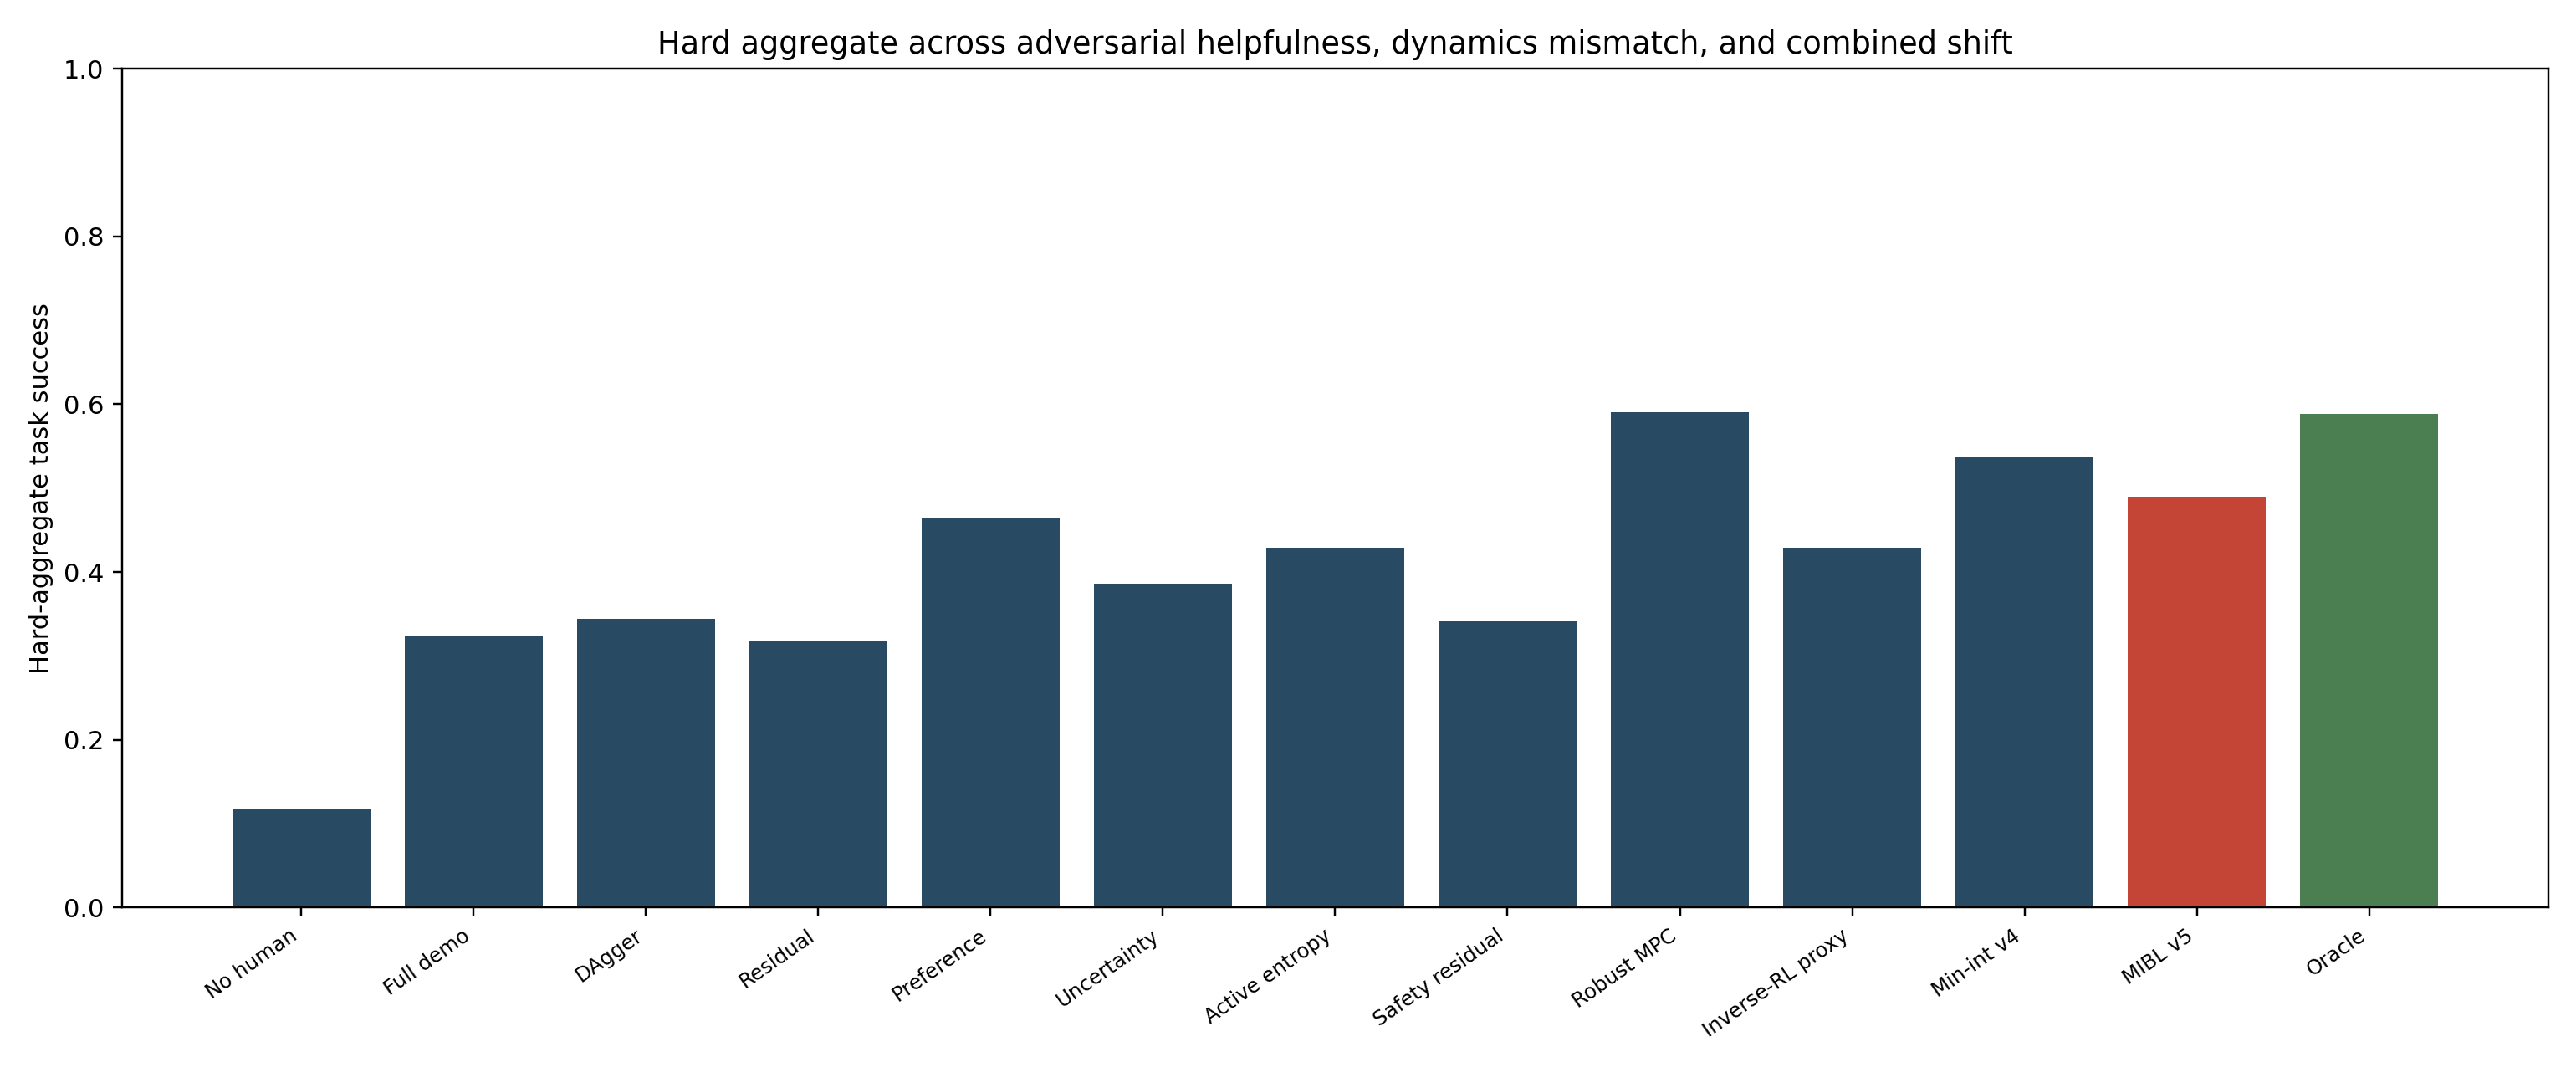
\includegraphics[width=0.96\linewidth]{minimum_intervention_hard_success_v5.png}\caption{Hard-aggregate success. MIBL v5 trails robust MPC and v4.}\label{fig:hard-success}\end{figure}
\begin{figure}[tbp]\centering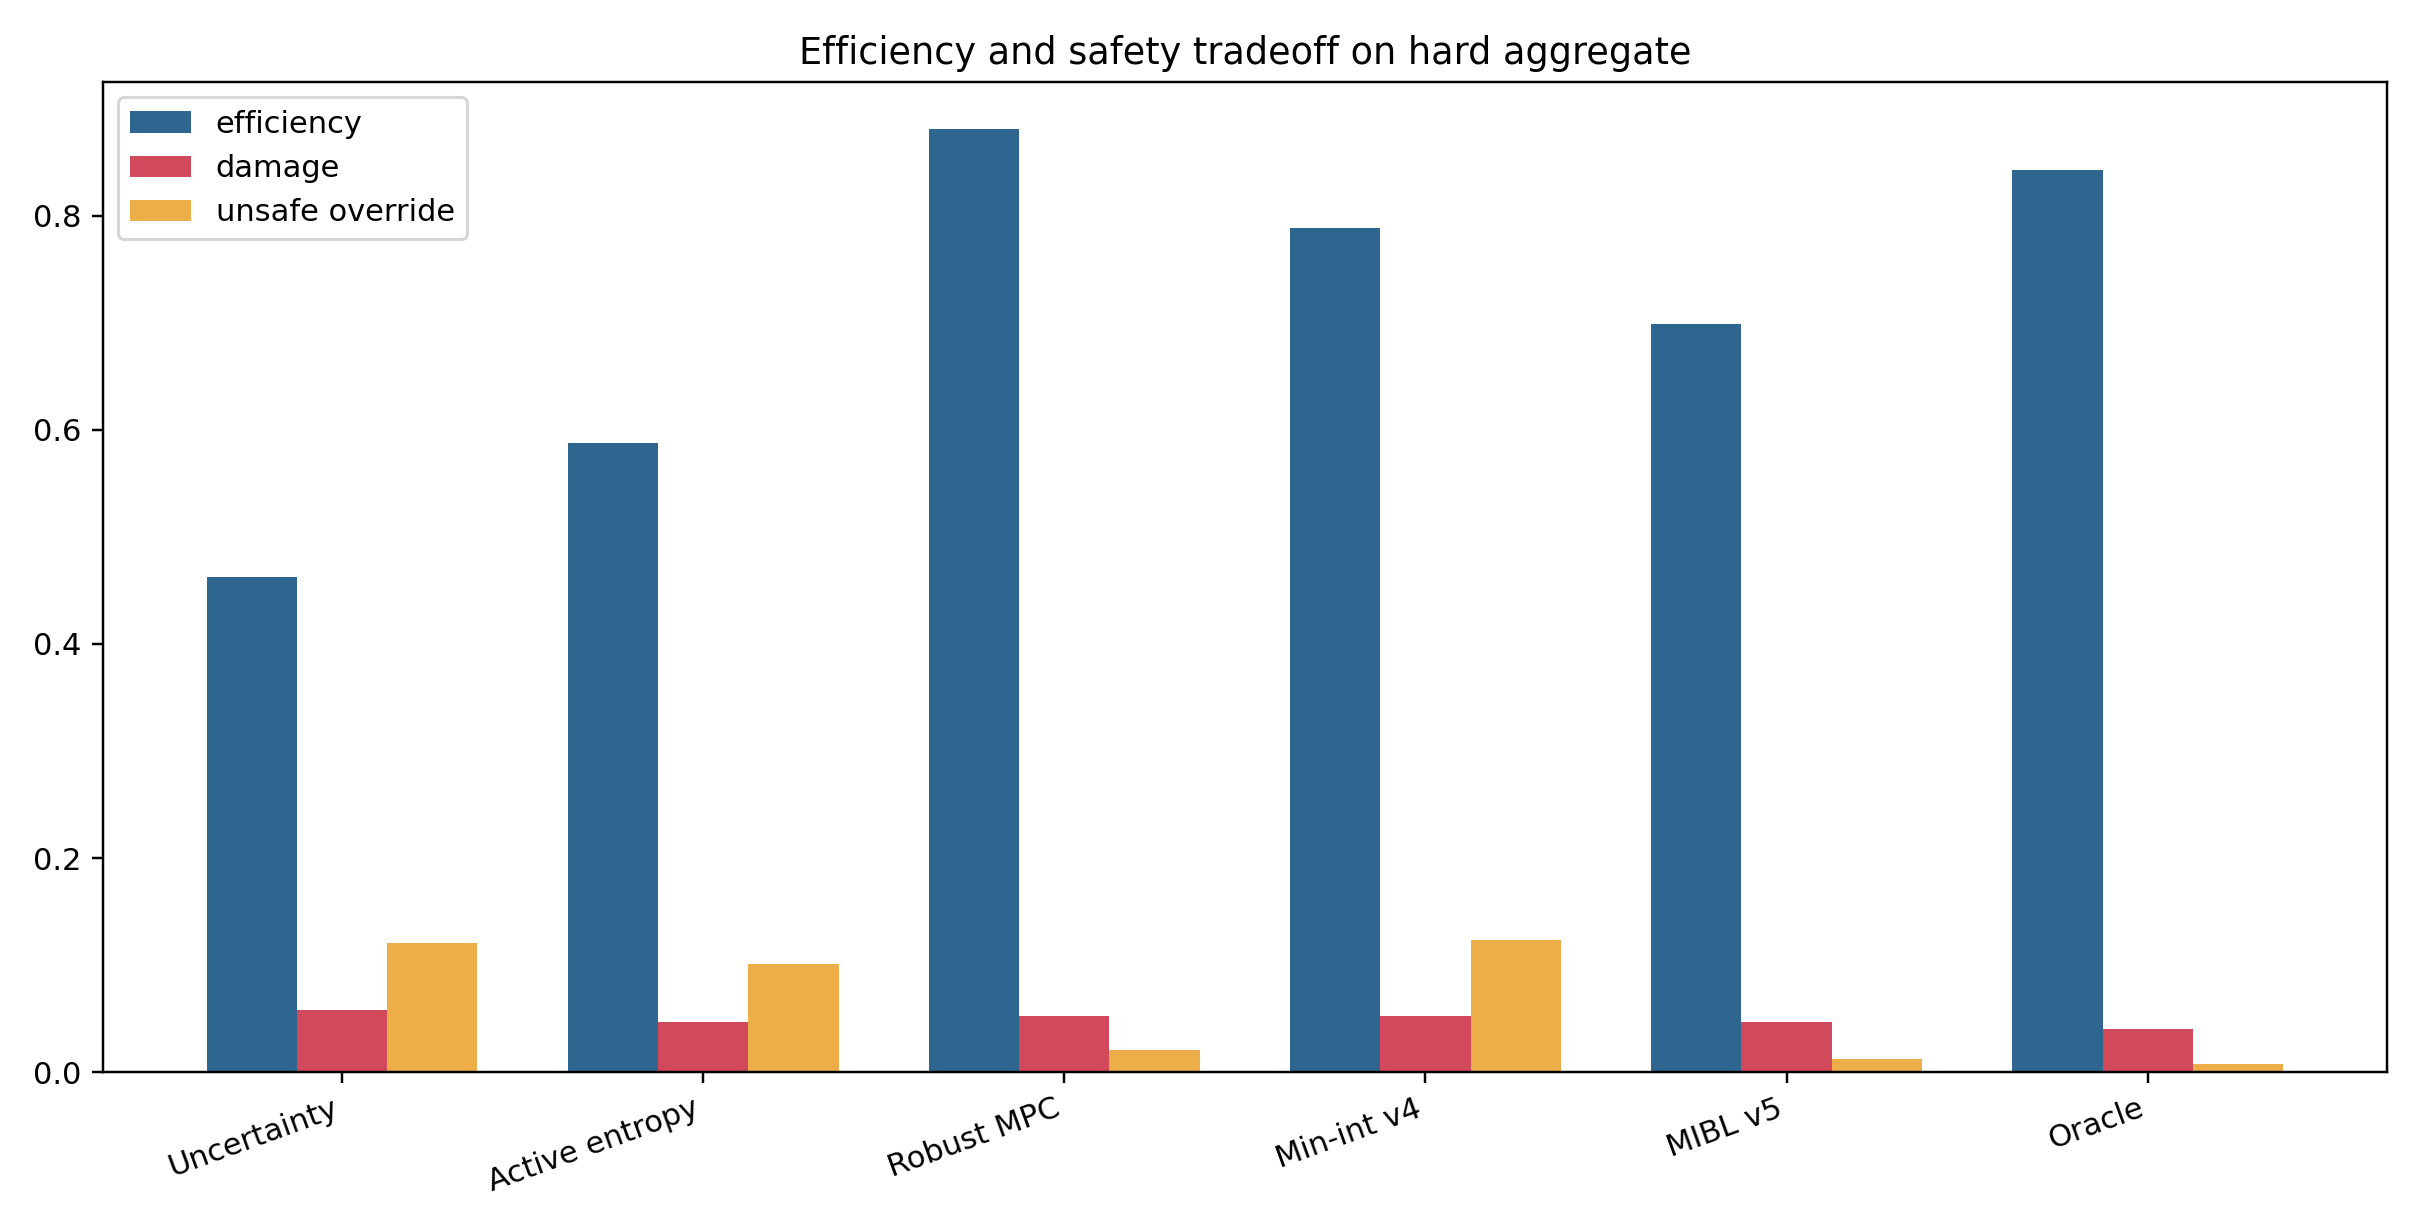
\includegraphics[width=0.88\linewidth]{minimum_intervention_safety_tradeoff_v5.png}\caption{Efficiency, damage, and unsafe override rates on the hard aggregate. V5 improves unsafe overrides but loses success and efficiency.}\label{fig:safety}\end{figure}
\begin{figure}[tbp]\centering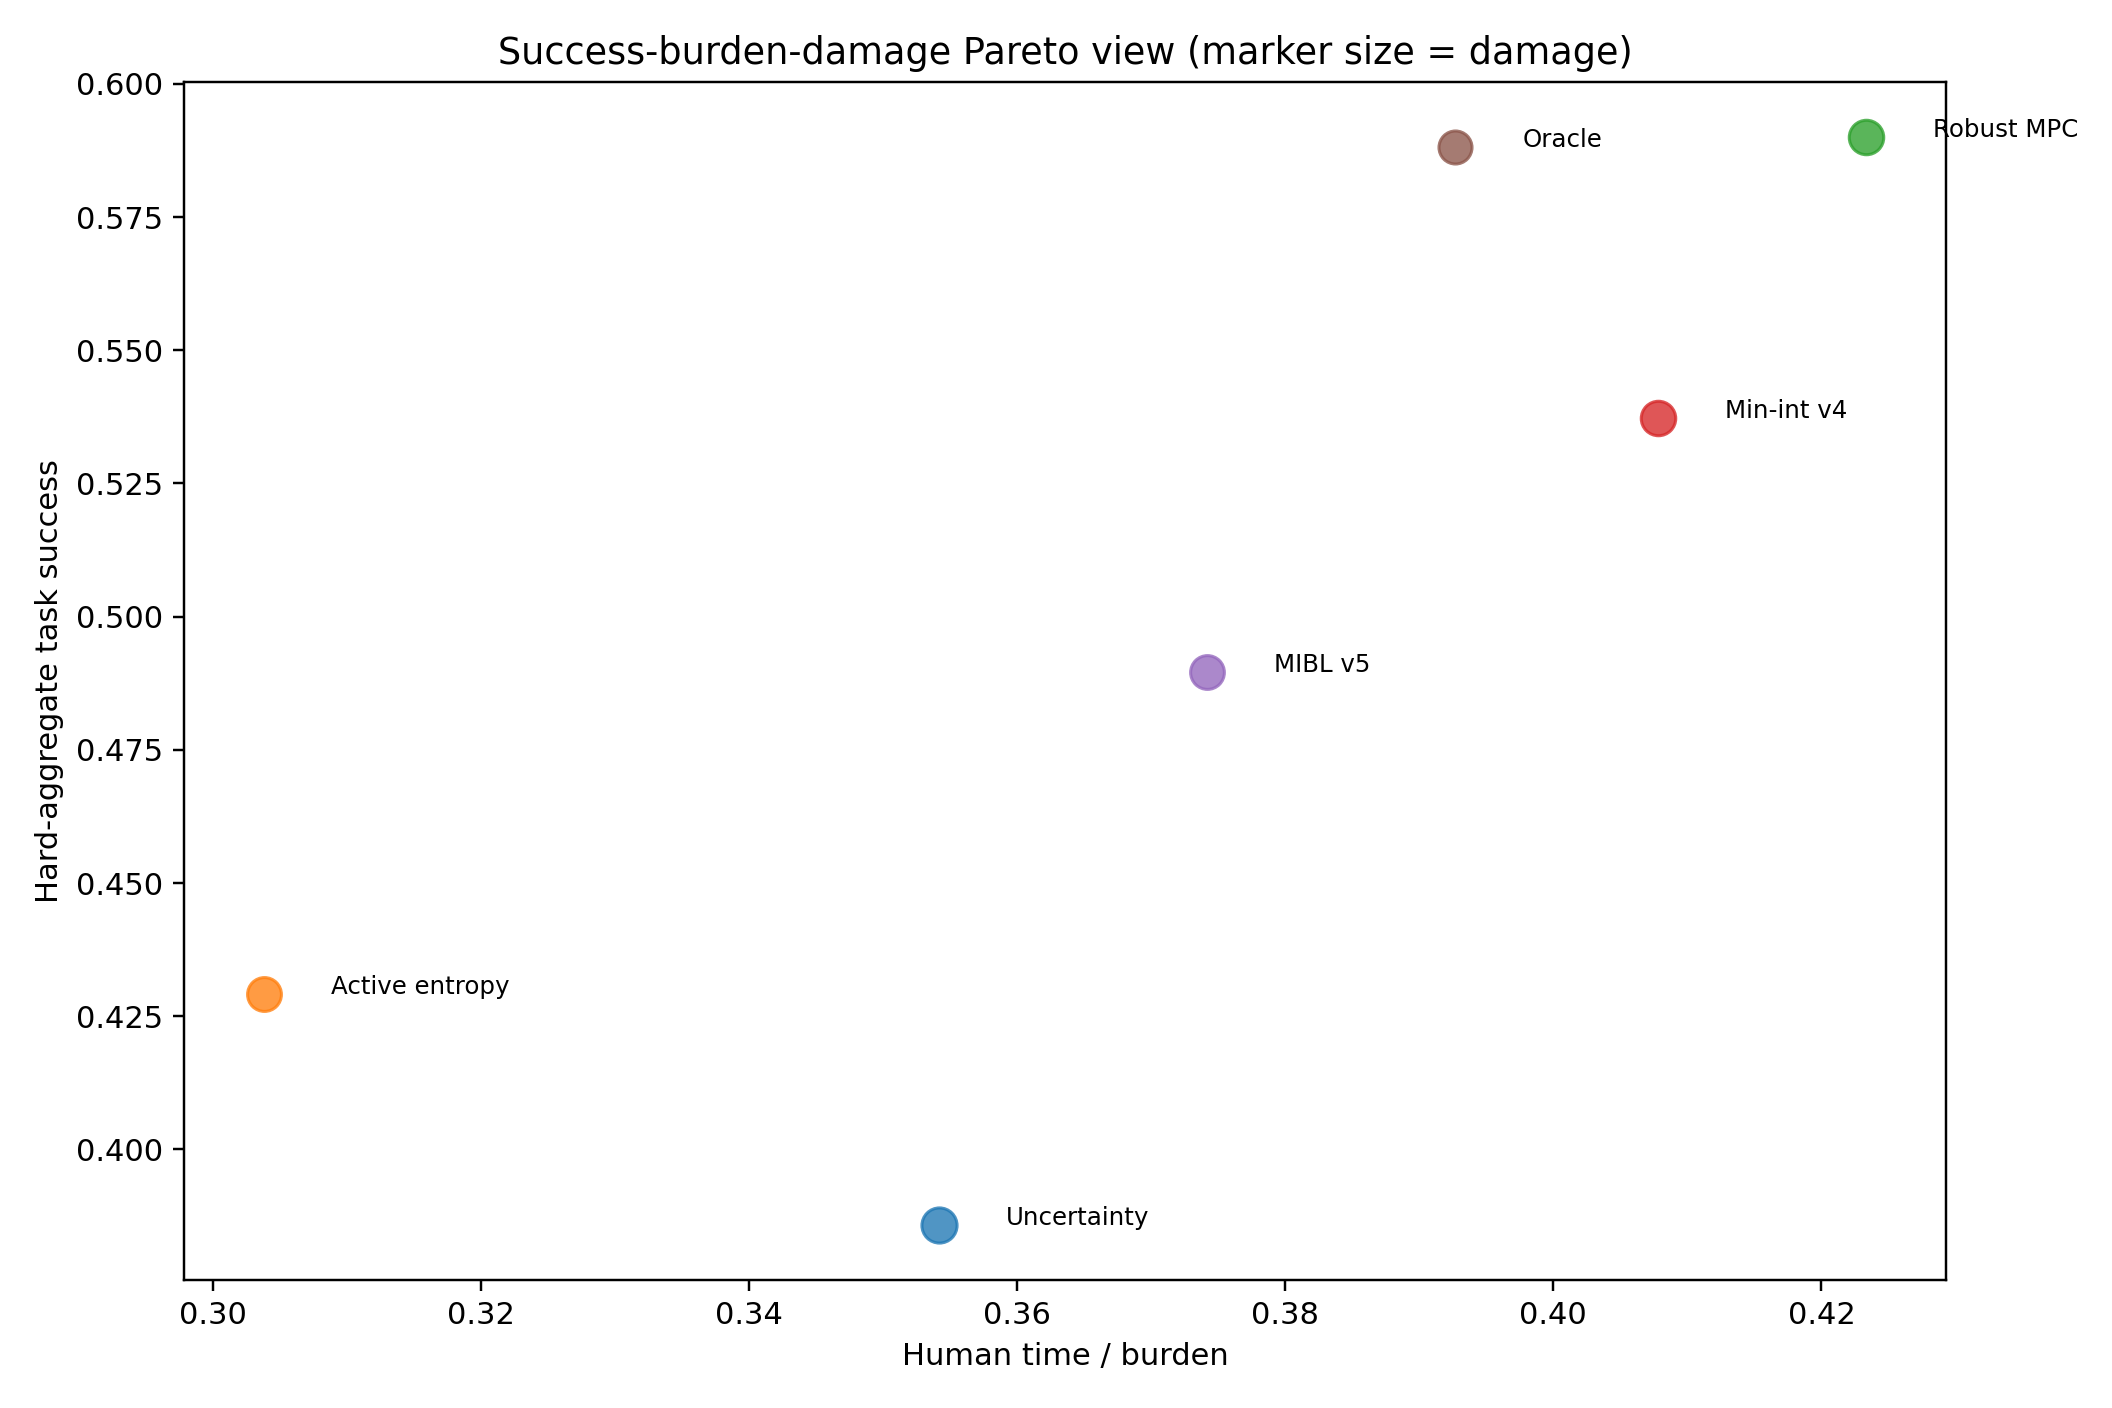
\includegraphics[width=0.82\linewidth]{minimum_intervention_pareto_v5.png}\caption{Success-burden-damage Pareto view. Marker size is damage.}\label{fig:pareto}\end{figure}
\section{Mechanism Ablations}
The mechanism gate is the most damaging result. The full v5 method does not dominate its own ablations. Removing the minimum-norm objective, removing the human-effort cost, removing safety override, and removing query throttling can all improve robust utility or task success in the hard ablation splits. This does not mean those ablations are deployable; it means the proposed mechanism is not uniquely validated.
\begin{center}
\scriptsize
\begin{longtable}{p{0.15\linewidth}p{0.39\linewidth}rrrr}
\caption{Mechanism ablations. The full mechanism was required to beat every non-full ablation on robust utility by at least 0.015.}\label{tab:ablation}\\
\toprule
Split & Ablation & Success & Efficiency & Damage & Utility\\
\midrule
\endfirsthead
\caption[]{Mechanism ablations. The full mechanism was required to beat every non-full ablation on robust utility by at least 0.015. (continued)}\\
\toprule
Split & Ablation & Success & Efficiency & Damage & Utility\\
\midrule
\endhead
Dynamics & full\_minimum\_intervention\_boundary\_learner\_v5 & 0.490 & 0.649 & 0.052 & 0.680\\
Dynamics & minus\_minimum\_norm\_objective & 0.575 & 0.774 & 0.049 & 0.788\\
Dynamics & minus\_counterfactual\_boundary & 0.431 & 0.552 & 0.040 & 0.611\\
Dynamics & minus\_intent\_preservation & 0.492 & 0.651 & 0.048 & 0.682\\
Dynamics & minus\_human\_effort\_cost & 0.580 & 0.785 & 0.046 & 0.795\\
Dynamics & minus\_safety\_override & 0.579 & 0.786 & 0.058 & 0.783\\
Dynamics & minus\_query\_throttling & 0.533 & 0.711 & 0.037 & 0.744\\
Dynamics & minus\_calibration & 0.515 & 0.685 & 0.045 & 0.716\\
Dynamics & all\_corrections\_imitation & 0.417 & 0.481 & 0.053 & 0.564\\
Dynamics & preference\_only\_objective & 0.474 & 0.623 & 0.057 & 0.655\\
Combined & full\_minimum\_intervention\_boundary\_learner\_v5 & 0.476 & 0.648 & 0.048 & 0.664\\
Combined & minus\_minimum\_norm\_objective & 0.543 & 0.756 & 0.055 & 0.744\\
Combined & minus\_counterfactual\_boundary & 0.435 & 0.567 & 0.041 & 0.616\\
Combined & minus\_intent\_preservation & 0.470 & 0.641 & 0.048 & 0.657\\
Combined & minus\_human\_effort\_cost & 0.551 & 0.774 & 0.055 & 0.758\\
Combined & minus\_safety\_override & 0.533 & 0.756 & 0.051 & 0.730\\
Combined & minus\_query\_throttling & 0.496 & 0.672 & 0.040 & 0.693\\
Combined & minus\_calibration & 0.497 & 0.680 & 0.047 & 0.692\\
Combined & all\_corrections\_imitation & 0.340 & 0.354 & 0.058 & 0.451\\
Combined & preference\_only\_objective & 0.448 & 0.604 & 0.067 & 0.613\\
\bottomrule
\end{longtable}
\normalsize
\end{center}
\begin{figure}[tbp]\centering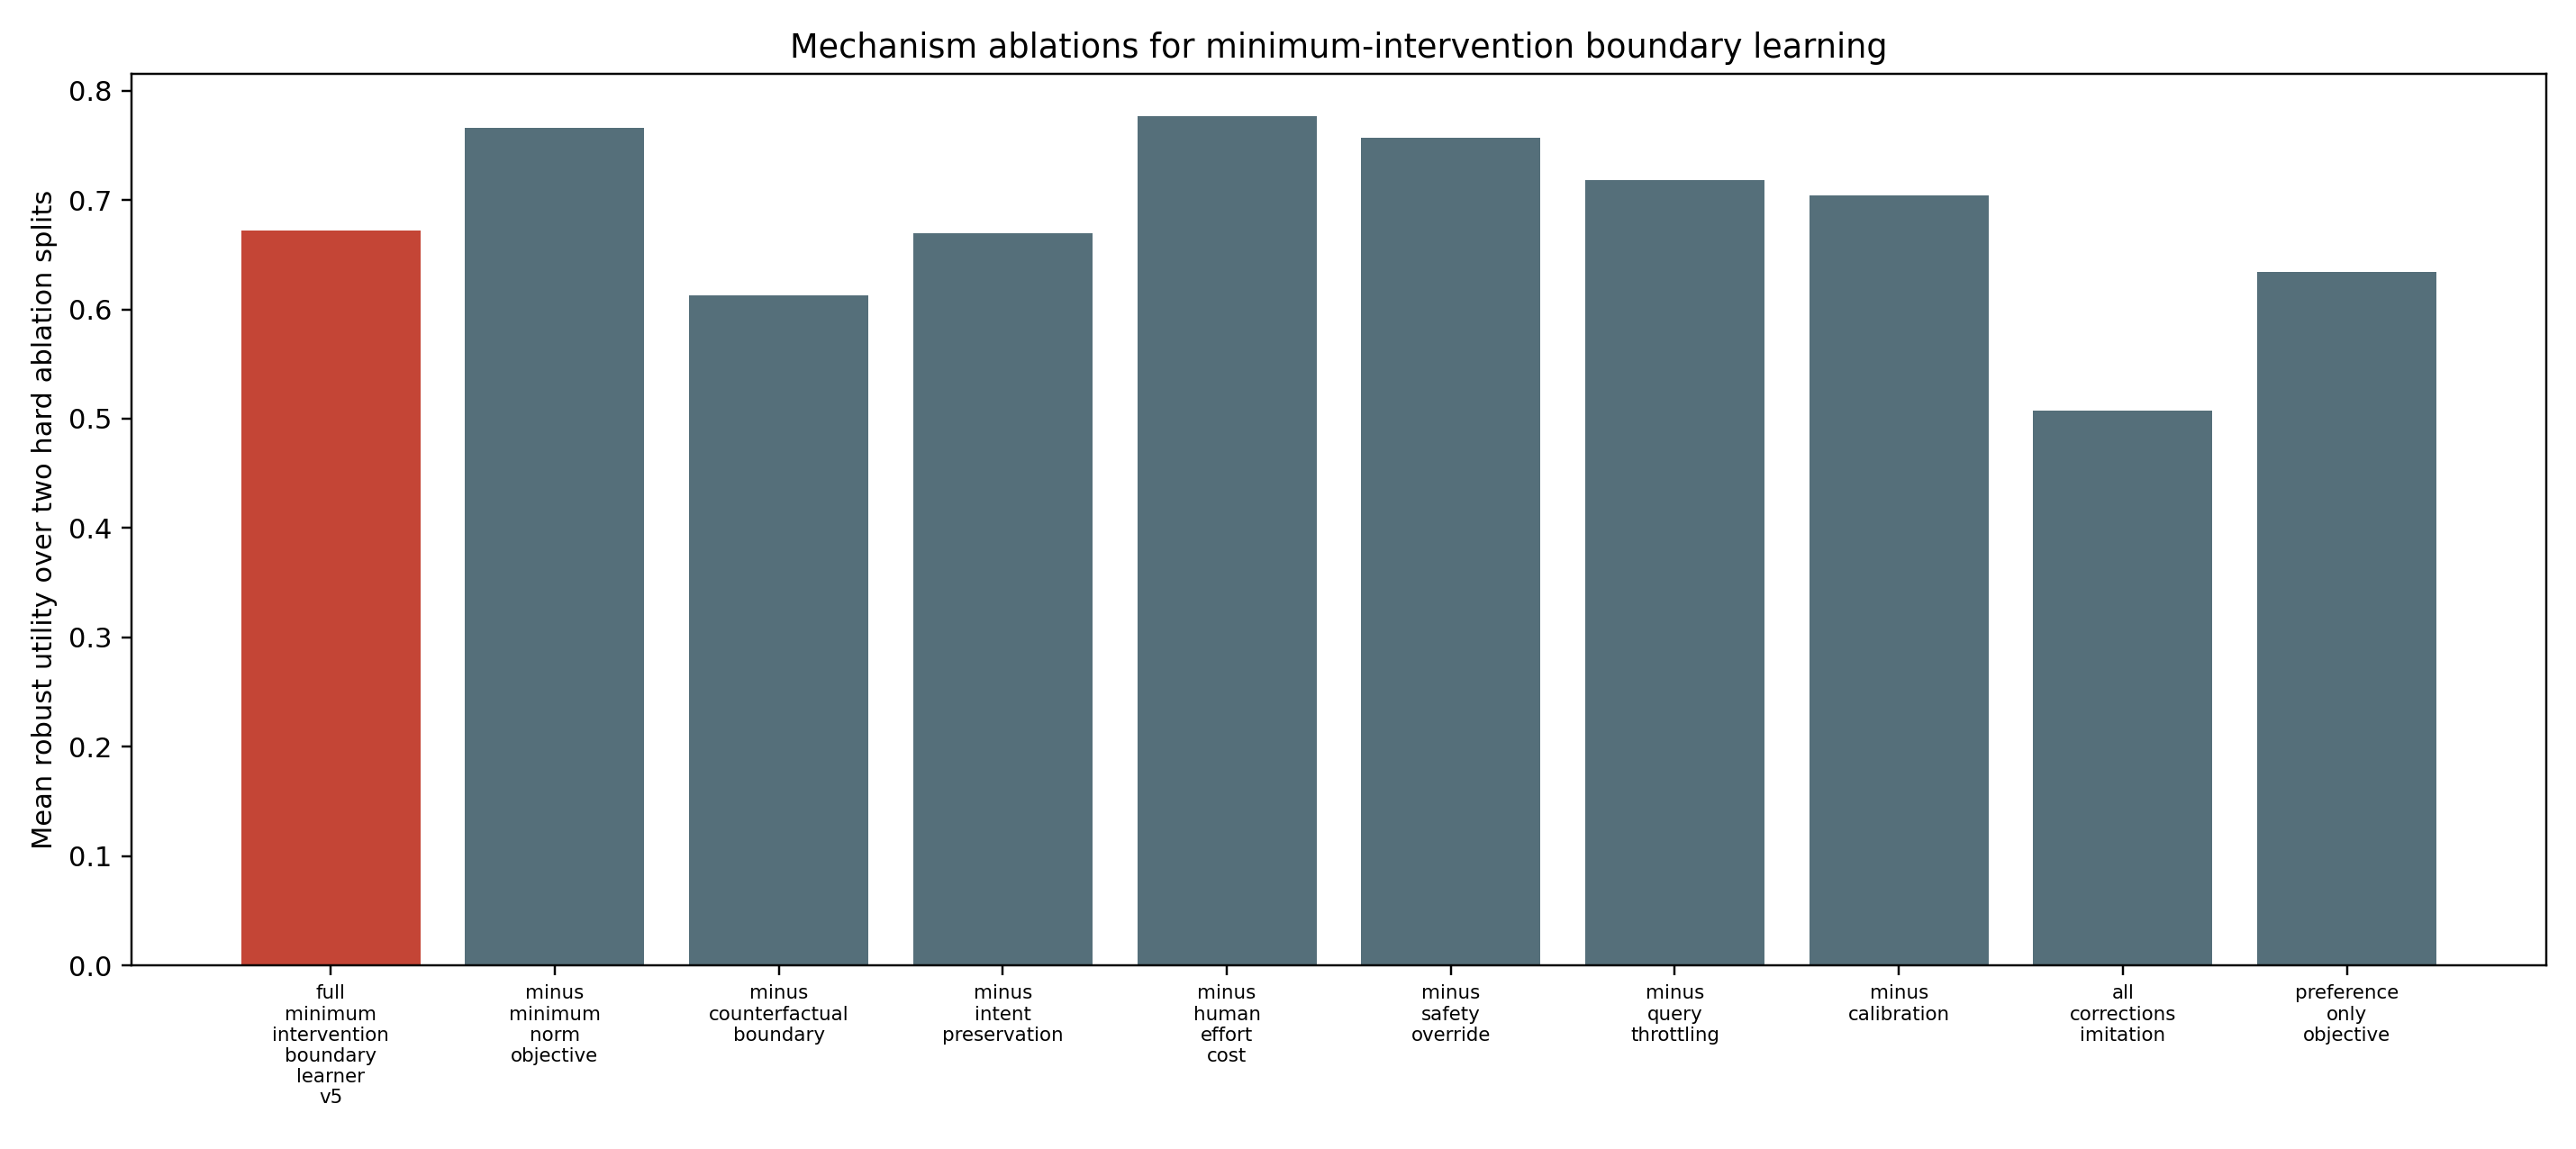
\includegraphics[width=0.96\linewidth]{minimum_intervention_ablation_v5.png}\caption{Ablation robust utility. The full mechanism fails the predeclared necessity margin.}\label{fig:ablation}\end{figure}
\section{Stress Tests}
The stress gate is the one gate v5 survives. At maximum combined stress, no non-oracle method Pareto-dominates v5 on success, efficiency, damage, and unsafe overrides. However, robust MPC still has higher success and utility, and a single stress-gate pass cannot rescue the failed main and mechanism gates.
\begin{center}
\scriptsize
\begin{longtable}{rp{0.26\linewidth}rrrrr}
\caption{Combined stress sweep. V5 was not Pareto-dominated at maximum stress, but that alone did not rescue the paper.}\label{tab:stress}\\
\toprule
Level & Method & Success & Efficiency & Damage & Unsafe & Utility\\
\midrule
\endfirsthead
\caption[]{Combined stress sweep. V5 was not Pareto-dominated at maximum stress, but that alone did not rescue the paper. (continued)}\\
\toprule
Level & Method & Success & Efficiency & Damage & Unsafe & Utility\\
\midrule
\endhead
0.0 & Full demo & 0.569 & 1.064 & 0.040 & 0.048 & 0.852\\
0.0 & Residual & 0.526 & 0.923 & 0.039 & 0.062 & 0.786\\
0.0 & Uncertainty query & 0.471 & 0.821 & 0.038 & 0.050 & 0.726\\
0.0 & Active entropy & 0.466 & 0.818 & 0.037 & 0.041 & 0.732\\
0.0 & Robust MPC & 0.599 & 1.289 & 0.034 & 0.000 & 0.957\\
0.0 & MIBL v5 & 0.579 & 1.146 & 0.035 & 0.000 & 0.925\\
0.0 & Oracle minimal & 0.630 & 1.251 & 0.036 & 0.000 & 0.986\\
0.2 & Full demo & 0.477 & 0.688 & 0.070 & 0.088 & 0.638\\
0.2 & Residual & 0.460 & 0.696 & 0.045 & 0.088 & 0.656\\
0.2 & Uncertainty query & 0.452 & 0.700 & 0.050 & 0.081 & 0.655\\
0.2 & Active entropy & 0.428 & 0.693 & 0.043 & 0.062 & 0.651\\
0.2 & Robust MPC & 0.587 & 1.130 & 0.034 & 0.001 & 0.902\\
0.2 & MIBL v5 & 0.545 & 0.973 & 0.040 & 0.000 & 0.843\\
0.2 & Oracle minimal & 0.634 & 1.145 & 0.037 & 0.000 & 0.958\\
0.4 & Full demo & 0.400 & 0.469 & 0.092 & 0.128 & 0.481\\
0.4 & Residual & 0.387 & 0.507 & 0.055 & 0.109 & 0.528\\
0.4 & Uncertainty query & 0.459 & 0.617 & 0.062 & 0.112 & 0.613\\
0.4 & Active entropy & 0.465 & 0.731 & 0.050 & 0.081 & 0.670\\
0.4 & Robust MPC & 0.585 & 0.983 & 0.036 & 0.009 & 0.858\\
0.4 & MIBL v5 & 0.522 & 0.845 & 0.045 & 0.000 & 0.770\\
0.4 & Oracle minimal & 0.615 & 0.989 & 0.042 & 0.001 & 0.895\\
0.6 & Full demo & 0.322 & 0.316 & 0.092 & 0.153 & 0.354\\
0.6 & Residual & 0.323 & 0.390 & 0.053 & 0.137 & 0.427\\
0.6 & Uncertainty query & 0.384 & 0.433 & 0.071 & 0.145 & 0.476\\
0.6 & Active entropy & 0.422 & 0.594 & 0.054 & 0.097 & 0.579\\
0.6 & Robust MPC & 0.548 & 0.828 & 0.044 & 0.018 & 0.772\\
0.6 & MIBL v5 & 0.476 & 0.696 & 0.048 & 0.006 & 0.680\\
0.6 & Oracle minimal & 0.609 & 0.890 & 0.046 & 0.001 & 0.856\\
0.8 & Full demo & 0.257 & 0.217 & 0.104 & 0.174 & 0.250\\
0.8 & Residual & 0.251 & 0.266 & 0.048 & 0.139 & 0.328\\
0.8 & Uncertainty query & 0.305 & 0.307 & 0.071 & 0.161 & 0.361\\
0.8 & Active entropy & 0.367 & 0.481 & 0.058 & 0.113 & 0.487\\
0.8 & Robust MPC & 0.552 & 0.765 & 0.055 & 0.030 & 0.746\\
0.8 & MIBL v5 & 0.453 & 0.605 & 0.052 & 0.019 & 0.624\\
0.8 & Oracle minimal & 0.580 & 0.777 & 0.046 & 0.013 & 0.791\\
1.0 & Full demo & 0.197 & 0.153 & 0.101 & 0.207 & 0.162\\
1.0 & Residual & 0.188 & 0.182 & 0.056 & 0.174 & 0.232\\
1.0 & Uncertainty query & 0.278 & 0.248 & 0.078 & 0.189 & 0.303\\
1.0 & Active entropy & 0.339 & 0.409 & 0.060 & 0.129 & 0.432\\
1.0 & Robust MPC & 0.518 & 0.660 & 0.061 & 0.053 & 0.673\\
1.0 & MIBL v5 & 0.435 & 0.532 & 0.059 & 0.040 & 0.574\\
1.0 & Oracle minimal & 0.583 & 0.723 & 0.055 & 0.024 & 0.767\\
\bottomrule
\end{longtable}
\normalsize
\end{center}
\begin{figure}[tbp]\centering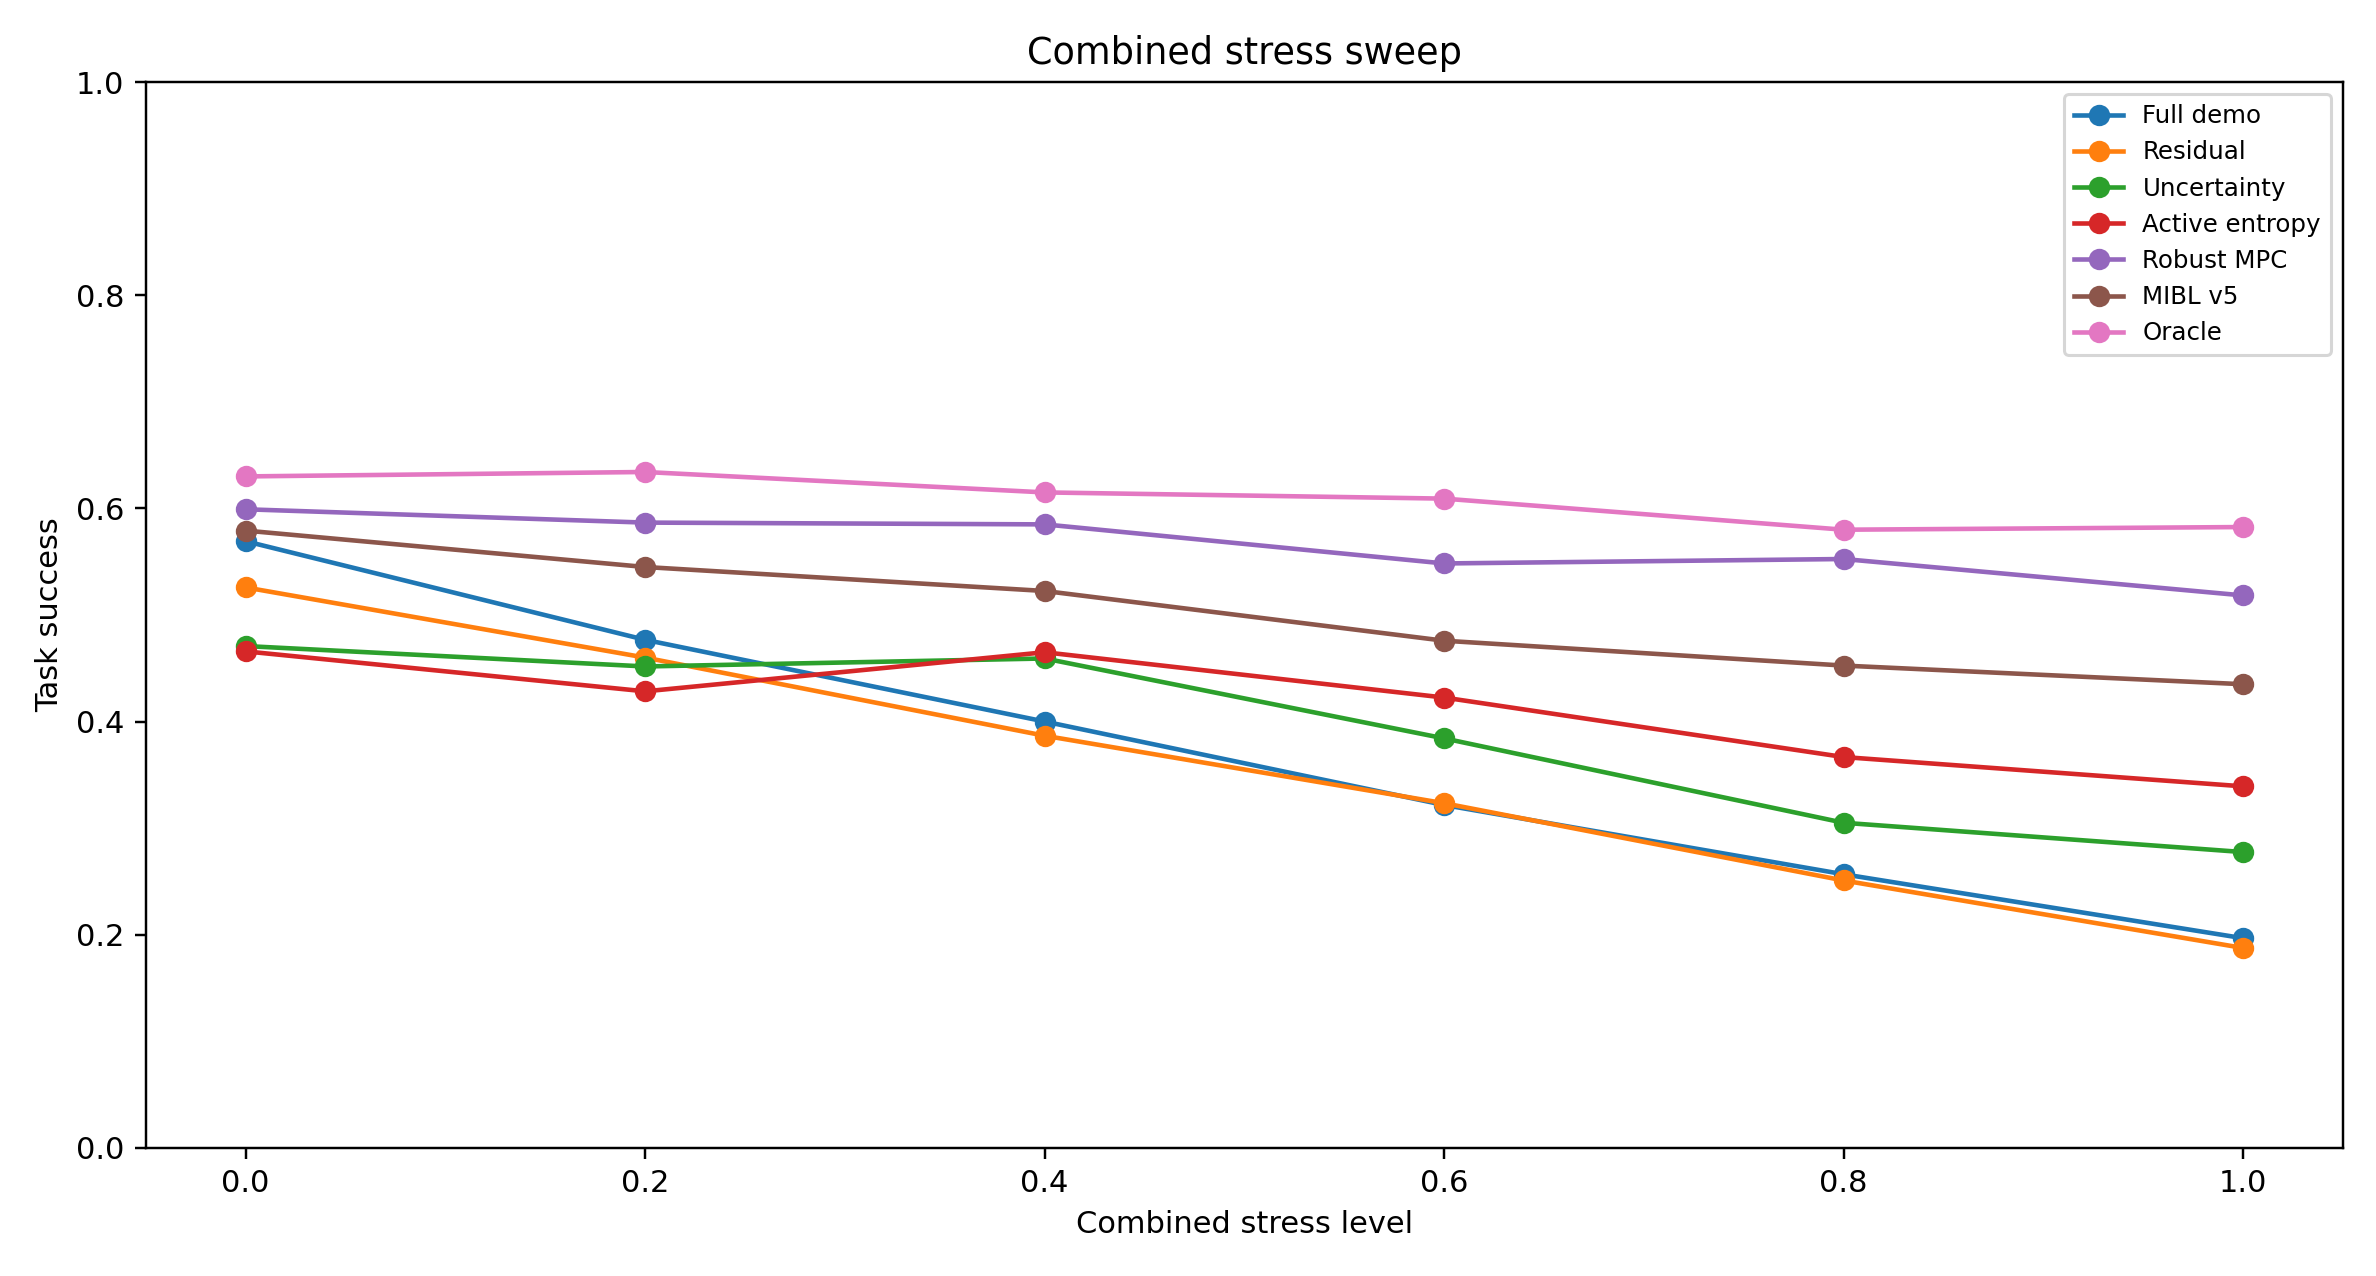
\includegraphics[width=0.90\linewidth]{minimum_intervention_stress_sweep_v5.png}\caption{Combined stress sweep. V5 is not dominated at maximum stress, but robust MPC keeps higher success.}\label{fig:stress}\end{figure}
\section{Fixed-Risk Deployment}
The fixed-risk protocol is intentionally harsh because deployment claims should be harsh. A method must decide when it is safe enough to accept autonomous execution under budgets 0.02, 0.05, 0.08, and 0.10. At budget 0.05, every method has zero accepted coverage on both fixed-risk splits. This means the calibrated risk scores do not support a nontrivial deployment claim.
\begin{center}
\scriptsize
\begin{longtable}{p{0.16\linewidth}rp{0.26\linewidth}rrrr}
\caption{Fixed-risk deployment tests. At budget 0.05 all non-oracle and oracle methods had zero accepted coverage, so the frozen fixed-risk gate failed.}\label{tab:fixed}\\
\toprule
Split & Budget & Method & Coverage & Succ. & Damage & Unsafe\\
\midrule
\endfirsthead
\caption[]{Fixed-risk deployment tests. At budget 0.05 all non-oracle and oracle methods had zero accepted coverage, so the frozen fixed-risk gate failed. (continued)}\\
\toprule
Split & Budget & Method & Coverage & Succ. & Damage & Unsafe\\
\midrule
\endhead
Combined & 0.02 & Active entropy & 0.000 & 0.000 & 0.000 & 0.000\\
Combined & 0.02 & MIBL v5 & 0.000 & 0.000 & 0.000 & 0.000\\
Combined & 0.02 & Oracle minimal & 0.000 & 0.000 & 0.000 & 0.000\\
Combined & 0.02 & Robust MPC & 0.000 & 0.000 & 0.000 & 0.000\\
Combined & 0.02 & Safety residual & 0.000 & 0.000 & 0.000 & 0.000\\
Combined & 0.02 & Uncertainty query & 0.000 & 0.000 & 0.000 & 0.000\\
Combined & 0.05 & Active entropy & 0.000 & 0.000 & 0.000 & 0.000\\
Combined & 0.05 & MIBL v5 & 0.000 & 0.000 & 0.000 & 0.000\\
Combined & 0.05 & Oracle minimal & 0.000 & 0.000 & 0.000 & 0.000\\
Combined & 0.05 & Robust MPC & 0.000 & 0.000 & 0.000 & 0.000\\
Combined & 0.05 & Safety residual & 0.000 & 0.000 & 0.000 & 0.000\\
Combined & 0.05 & Uncertainty query & 0.000 & 0.000 & 0.000 & 0.000\\
Combined & 0.10 & Active entropy & 0.000 & 0.000 & 0.000 & 0.000\\
Combined & 0.10 & MIBL v5 & 0.000 & 0.000 & 0.000 & 0.000\\
Combined & 0.10 & Oracle minimal & 0.997 & 0.583 & 0.046 & 0.008\\
Combined & 0.10 & Robust MPC & 0.000 & 0.000 & 0.000 & 0.000\\
Combined & 0.10 & Safety residual & 0.000 & 0.000 & 0.000 & 0.000\\
Combined & 0.10 & Uncertainty query & 0.000 & 0.000 & 0.000 & 0.000\\
Dynamics & 0.02 & Active entropy & 0.000 & 0.000 & 0.000 & 0.000\\
Dynamics & 0.02 & MIBL v5 & 0.000 & 0.000 & 0.000 & 0.000\\
Dynamics & 0.02 & Oracle minimal & 0.000 & 0.000 & 0.000 & 0.000\\
Dynamics & 0.02 & Robust MPC & 0.000 & 0.000 & 0.000 & 0.000\\
Dynamics & 0.02 & Safety residual & 0.000 & 0.000 & 0.000 & 0.000\\
Dynamics & 0.02 & Uncertainty query & 0.000 & 0.000 & 0.000 & 0.000\\
Dynamics & 0.05 & Active entropy & 0.000 & 0.000 & 0.000 & 0.000\\
Dynamics & 0.05 & MIBL v5 & 0.000 & 0.000 & 0.000 & 0.000\\
Dynamics & 0.05 & Oracle minimal & 0.000 & 0.000 & 0.000 & 0.000\\
Dynamics & 0.05 & Robust MPC & 0.000 & 0.000 & 0.000 & 0.000\\
Dynamics & 0.05 & Safety residual & 0.000 & 0.000 & 0.000 & 0.000\\
Dynamics & 0.05 & Uncertainty query & 0.000 & 0.000 & 0.000 & 0.000\\
Dynamics & 0.10 & Active entropy & 0.000 & 0.000 & 0.000 & 0.000\\
Dynamics & 0.10 & MIBL v5 & 0.000 & 0.000 & 0.000 & 0.000\\
Dynamics & 0.10 & Oracle minimal & 1.000 & 0.567 & 0.039 & 0.017\\
Dynamics & 0.10 & Robust MPC & 0.000 & 0.000 & 0.000 & 0.000\\
Dynamics & 0.10 & Safety residual & 0.000 & 0.000 & 0.000 & 0.000\\
Dynamics & 0.10 & Uncertainty query & 0.000 & 0.000 & 0.000 & 0.000\\
\bottomrule
\end{longtable}
\normalsize
\end{center}
\begin{figure}[tbp]\centering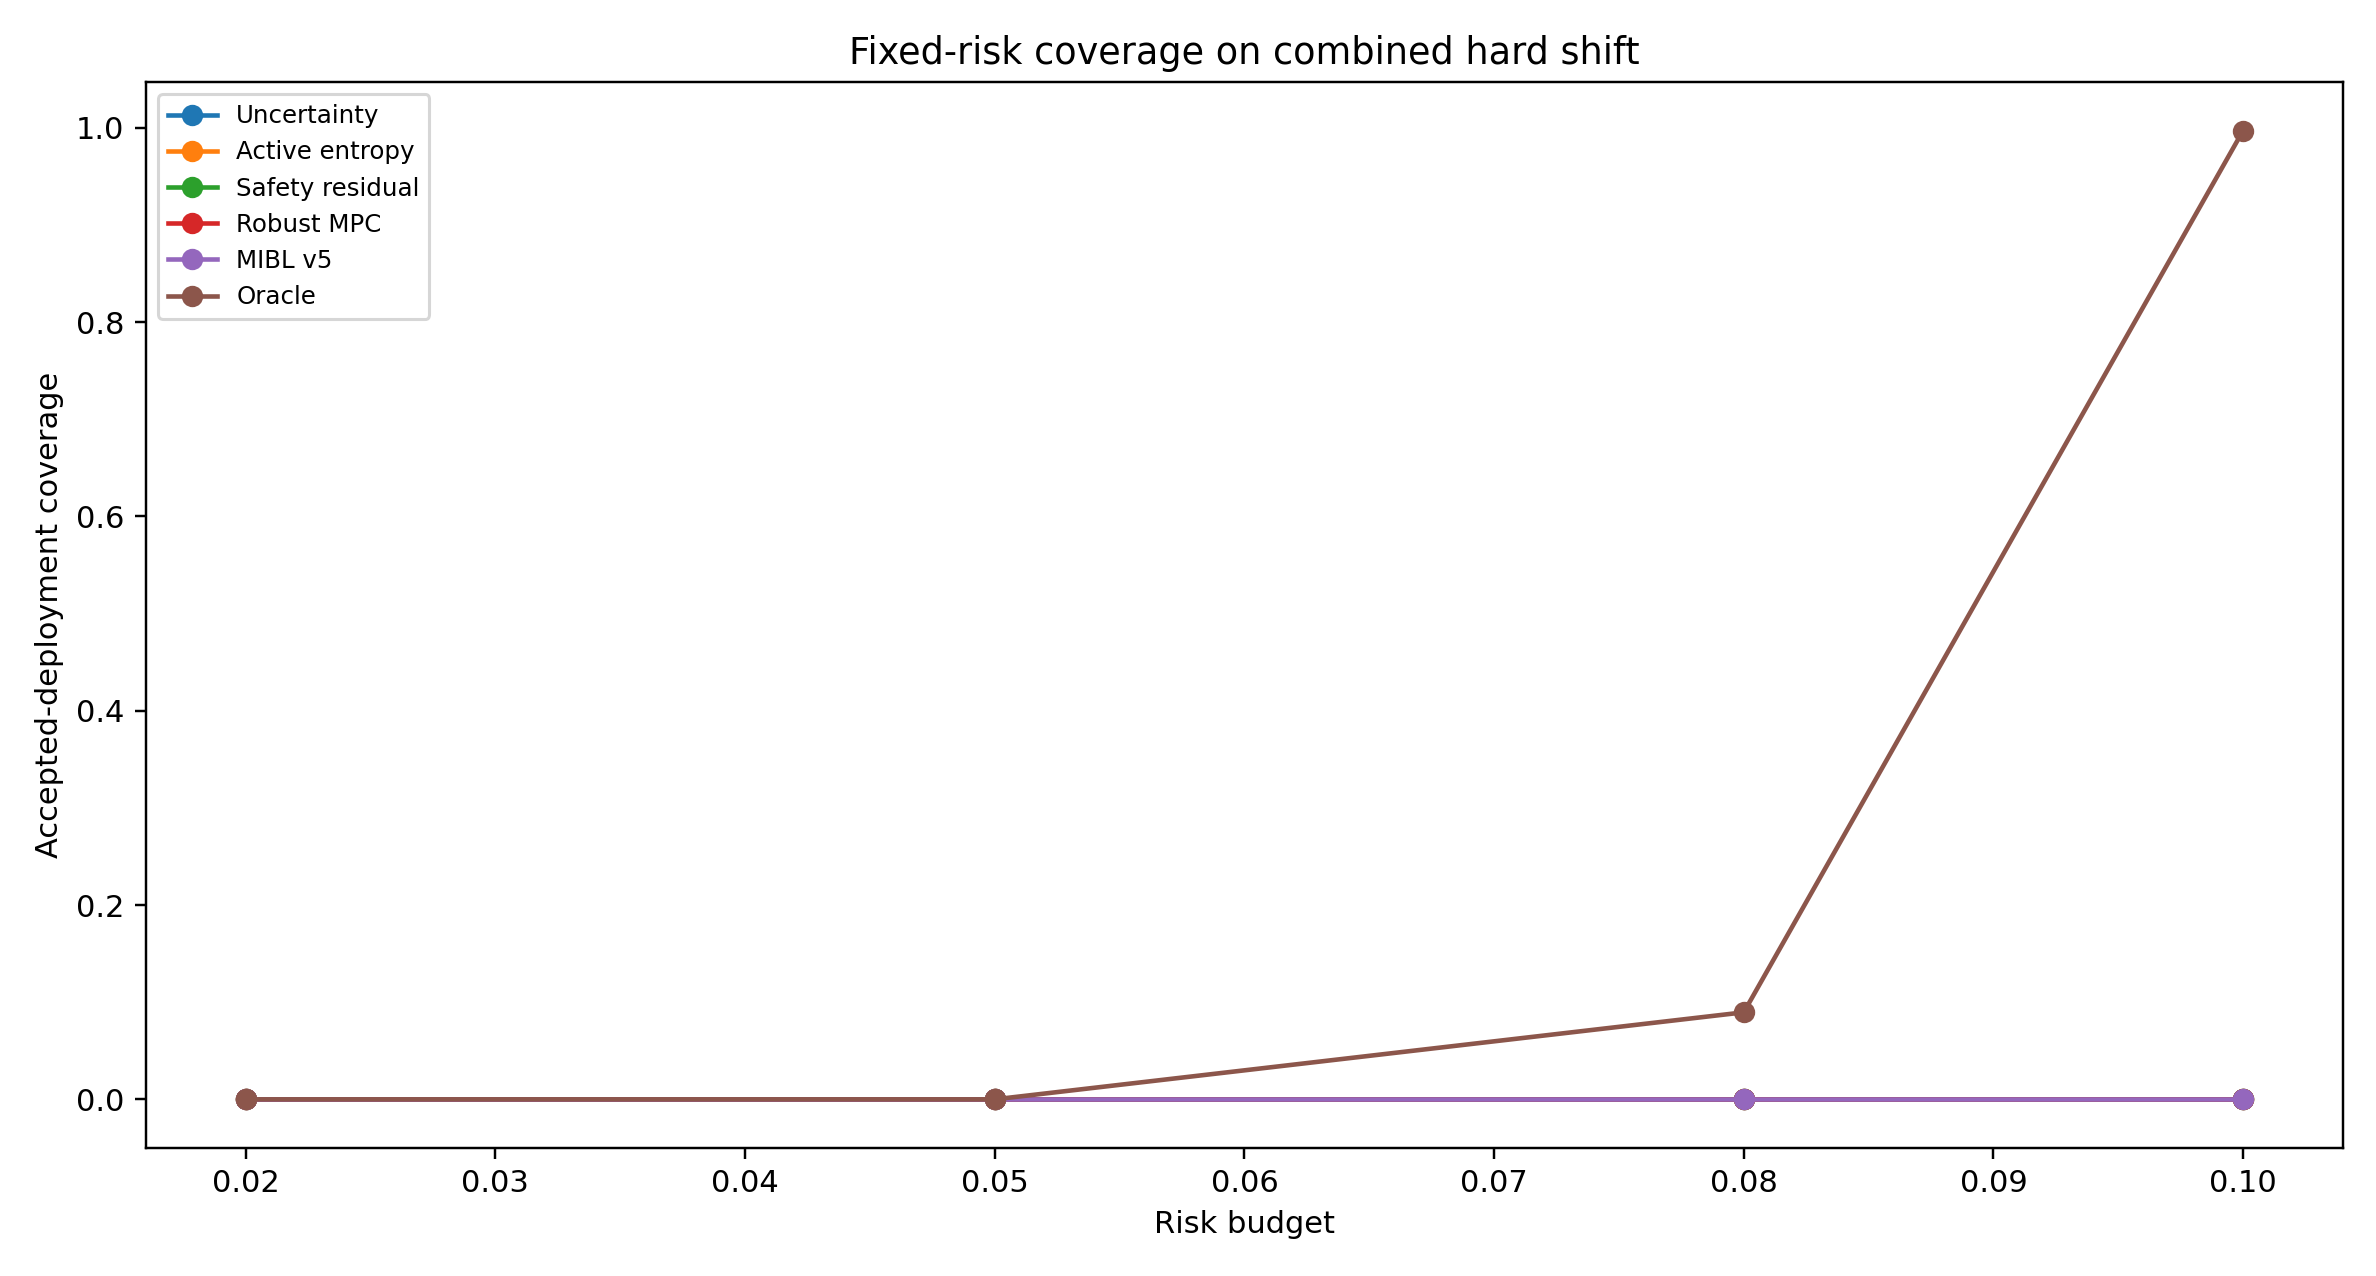
\includegraphics[width=0.90\linewidth]{minimum_intervention_fixed_risk_v5.png}\caption{Fixed-risk coverage on combined hard shift. Strict budget 0.05 gives zero coverage.}\label{fig:fixed}\end{figure}
\section{Negative Cases}
Negative cases are retained because they prevent a visually polished but brittle paper. They cover safety conflicts, semantic goal ambiguity, nonlocal deformable dynamics, adversarial helpfulness, delayed boundary shifts, and under-correction. These cases explain why a small correction is not automatically a correct correction.
\begin{center}
\scriptsize
\begin{longtable}{p{0.25\linewidth}p{0.25\linewidth}p{0.38\linewidth}}
\caption{Retained negative cases used to keep the discussion honest.}\label{tab:negative}\\
\toprule
Case & Family & Terminal lesson\\
\midrule
\endfirsthead
\caption[]{Retained negative cases used to keep the discussion honest. (continued)}\\
\toprule
Case & Family & Terminal lesson\\
\midrule
\endhead
safety\_conflict\_0 & safety\_conflict & minimality cannot replace a safety constraint\\
safety\_conflict\_1 & safety\_conflict & minimality cannot replace a safety constraint\\
safety\_conflict\_2 & safety\_conflict & minimality cannot replace a safety constraint\\
safety\_conflict\_3 & safety\_conflict & minimality cannot replace a safety constraint\\
semantic\_goal\_ambiguity\_0 & semantic\_goal\_ambiguity & physical boundary evidence is under-specified\\
semantic\_goal\_ambiguity\_1 & semantic\_goal\_ambiguity & physical boundary evidence is under-specified\\
semantic\_goal\_ambiguity\_2 & semantic\_goal\_ambiguity & physical boundary evidence is under-specified\\
semantic\_goal\_ambiguity\_3 & semantic\_goal\_ambiguity & physical boundary evidence is under-specified\\
nonlocal\_deformable\_dynamics\_0 & nonlocal\_deformable\_dynamics & needs high-fidelity dynamics\\
nonlocal\_deformable\_dynamics\_1 & nonlocal\_deformable\_dynamics & needs high-fidelity dynamics\\
nonlocal\_deformable\_dynamics\_2 & nonlocal\_deformable\_dynamics & needs high-fidelity dynamics\\
nonlocal\_deformable\_dynamics\_3 & nonlocal\_deformable\_dynamics & needs high-fidelity dynamics\\
adversarial\_helpfulness\_0 & adversarial\_helpfulness & helpfulness must be modeled explicitly\\
adversarial\_helpfulness\_1 & adversarial\_helpfulness & helpfulness must be modeled explicitly\\
adversarial\_helpfulness\_2 & adversarial\_helpfulness & helpfulness must be modeled explicitly\\
adversarial\_helpfulness\_3 & adversarial\_helpfulness & helpfulness must be modeled explicitly\\
delayed\_boundary\_shift\_0 & delayed\_boundary\_shift & delay can invert the apparent minimal action\\
delayed\_boundary\_shift\_1 & delayed\_boundary\_shift & delay can invert the apparent minimal action\\
delayed\_boundary\_shift\_2 & delayed\_boundary\_shift & delay can invert the apparent minimal action\\
delayed\_boundary\_shift\_3 & delayed\_boundary\_shift & delay can invert the apparent minimal action\\
under\_correction\_0 & under\_correction & pure minimum norm can under-correct\\
under\_correction\_1 & under\_correction & pure minimum norm can under-correct\\
under\_correction\_2 & under\_correction & pure minimum norm can under-correct\\
under\_correction\_3 & under\_correction & pure minimum norm can under-correct\\
\bottomrule
\end{longtable}
\normalsize
\end{center}
\section{Prior-Work Boundary}
The local literature pool is used as a hostile-review pressure map. The paper sits near active correction, residual learning, preference learning, MPC, risk calibration, and robot manipulation datasets \citep{pool85_07,pool85_08,pool85_09,pool85_10,pool85_11,pool85_12,pool85_13}. Because this rebuild has no real robot benchmark, it cannot claim to beat those bodies of work directly.
\begin{center}
\scriptsize
\begin{longtable}{p{0.12\linewidth}p{0.53\linewidth}p{0.08\linewidth}p{0.18\linewidth}}
\caption{Local prior-work pressure map. The entries are used as threat coverage, not as exhaustive manual survey.}\label{tab:prior}\\
\toprule
Cite & Prior-work pressure & Year & Source\\
\midrule
\endfirsthead
\caption[]{Local prior-work pressure map. The entries are used as threat coverage, not as exhaustive manual survey. (continued)}\\
\toprule
Cite & Prior-work pressure & Year & Source\\
\midrule
\endhead
\citep{pool85_01} & Towards understanding and synthesis of contact-rich anthropomorphic motions through interactive cyber-physical human & 2022 & Frontiers in Robotics and AI\\
\citep{pool85_02} & Interactive Force Control Based on Multimodal Robot Skin for Physical HumanRobot Collaboration & 2022 & Advanced Intelligent Systems\\
\citep{pool85_03} & Toward Zero-Human-Intervention Autonomous Robot Learning: A Continuous Result-Driven Self-Reward and Correction Framewor &  & crossref\\
\citep{pool85_04} & Human-Robot Interactive Skill Learning and Correction for Polishing Based on Dynamic Time Warping Iterative Learning Con & 2024 & IEEE Transactions on Control Systems Technology\\
\citep{pool85_05} & Immersive and interactive cyber-physical system (I2CPS) and virtual reality interface for human involved robotic manufac & 2021 & Journal of Manufacturing Systems\\
\citep{pool85_06} & Formal verification of physical human-robot interaction using interactive theorem proving & 2026 & Journal of Intelligent Systems\\
\citep{pool85_07} & A glass-box interactive machine learning approach for solving NP-hard problems with the human-in-the-loop & 2019 & Creative Mathematics and Informatics\\
\citep{pool85_08} & A glass-box interactive machine learning approach for solving NP-hard\textbackslash{}n problems with the human-in-the-lo & 2017 & arXiv (Cornell University)\\
\citep{pool85_09} & Bidirectional Human-Robot Communication for Physical Human-Robot Interaction & 2026 & arXiv\\
\citep{pool85_10} & Physical Human Interactive Guidance: Identifying Grasping Principles From Human-Planned Grasps & 2012 & IEEE Transactions on Robotics\\
\citep{pool85_11} & Predicting Tactile Sensory Outcome of Physical Human-Robot Interaction Through Embodied Learning Strategy & 2026 & IEEE Robotics and Automation Letters\\
\citep{pool85_12} & Interactive Learning via Physical Human Feedback Using Uncertainty-Aware Energy Tanks & 2026 & IEEE Robotics and Automation Letters\\
\citep{pool85_13} & A 3DGS and LLM-based physical-to-virtual approach for human-robot interactive manufacturing & 2025 & Manufacturing Letters\\
\citep{pool85_14} & Correction to "ArtistDirectable Motion Generation Using Overlapping Minimum Jerk Trajectories for Interactive Embodied S & 2026 & Computer Animation and Virtual Worlds\\
\citep{pool85_15} & Interactive and Immersive Process-Level Digital Twin for Collaborative Human-Robot Construction Work & 2021 & Journal of Computing in Civil Engineering\\
\citep{pool85_16} & Digital Twin for Human-Robot Interactive Welding and Welder Behavior Analysis & 2020 & IEEE/CAA Journal of Automatica Sinica\\
\citep{pool85_17} & Large Language Model-Driven 3D Hyper-Realistic Interactive Intelligent Digital Human System & 2025 & Sensors\\
\citep{pool85_18} & Interactive classifier system for real robot learning & 2002 & openalex\\
\citep{pool85_19} & Interactive machine learning: experimental evidence for the human in the algorithmic loop & 2018 & Applied Intelligence\\
\citep{pool85_20} & Learning Physical Human-Robot Interaction With Coupled Cooperative Primitives for a Lower Exoskeleton & 2019 & IEEE Transactions on Automation Science and Engineering\\
\citep{pool85_21} & Unified Learning from Demonstrations, Corrections, and Preferences during Physical Human-Robot Interaction & 2024 & ACM Transactions on Human-Robot Interaction\\
\citep{pool85_22} & Digital Twin-Driven Virtual Control Technology of Home-Use Robot: Human-Cyber-Physical System & 2022 & openalex\\
\citep{pool85_23} & Eye-Tracking in Physical Human-Robot Interaction: Mental Workload and Performance Prediction & 2023 & Human Factors The Journal of the Human Factors and Ergonomic\\
\citep{pool85_24} & Physical Human Interactive Guidance: Identifying Grasping Principles from Human-Planned Grasps & 2014 & Springer Tracts in Advanced Robotics The Human Hand as an In\\
\citep{pool85_25} & Physical interaction as communication: Learning robot objectives online from human corrections & 2022 & The International Journal of Robotics Research\\
\citep{pool85_26} & Exercising with Baxter: preliminary support for assistive social-physical human-robot interaction & 2020 & Journal of NeuroEngineering and Rehabilitation\\
\citep{pool85_27} & Collision Detection and Reaction: A Contribution to Safe Physical Human-Robot Interaction & 2008 & openalex\\
\citep{pool85_28} & Cooperative Transportation With Mobile Manipulator: A Capability Map-Based Framework for Physical Human-Robot Collaborat & 2022 & IEEE/ASME Transactions on Mechatronics\\
\citep{pool85_29} & Wireless MultistimulusResponsive FabricBased Actuators for Soft Robotic, Human-Machine Interactive, and Wearable Applica & 2020 & Advanced Materials Technologies\\
\citep{pool85_30} & Real Robot Learning with Human Teaching & 2002 & Tokyo Tech Research Repository (Tokyo Institute of Technolog\\
\citep{pool85_31} & A Machine Learning Approach to Resolving Conflicts in Physical Human-Robot Interaction & 2025 & ACM Transactions on Human-Robot Interaction\\
\citep{pool85_32} & Humans modulate arm stiffness to facilitate motor communication during overground physical human-robot interaction & 2022 & Scientific Reports\\
\citep{pool85_33} & Prediction of the Upper Limb Motion Based on a Geometrical Muscle Changes for Physical Human Machine Interaction & 2010 & Journal of Institute of Control, Robotics and Systems\\
\citep{pool85_34} & Human Posture Prediction During Physical Human-Robot Interaction & 2021 & IEEE Robotics and Automation Letters\\
\citep{pool85_35} & User intent estimation during robot learning using physical human robot interaction primitives & 2022 & Autonomous Robots\\
\citep{pool85_36} & Evolution of Industrial Robots from the Perspective of the Metaverse: Integration of Virtual and Physical Realities and  & 2024 & Applied Sciences\\
\citep{pool85_37} & Domestic Robots and the Dream of Automation: Understanding Human Interaction and Intervention & 2021 & openalex\\
\citep{pool85_38} & Integrating Perceptions: A Human-Centered Physical Safety Model for Human-Robot Interaction & 2025 & 2025 34th IEEE International Conference on Robot and Human I\\
\citep{pool85_39} & Contact and Physical Interaction & 2022 & Annual Review of Control, Robotics, and Autonomous Systems\\
\citep{pool85_40} & Interactive Learning from Policy-Dependent Human Feedback & 2017 & arXiv\\
\citep{pool85_41} & Learning from Demonstrations in Human-Robot Collaborative Scenarios: A Survey & 2022 & Robotics\\
\citep{pool85_42} & Deep Reinforcement Learning with Interactive Feedback in a Human-Robot Environment & 2020 & Own your potential (DEAKIN)\\
\citep{pool85_43} & Deep Reinforcement Learning with Interactive Feedback in a Human-Robot Environment & 2020 & Applied Sciences\\
\citep{pool85_44} & A robot for overground physical human-robot interaction experiments & 2022 & PLoS ONE\\
\citep{pool85_45} & Intrinsic interactive reinforcement learning - Using error-related potentials for real world human-robot interaction & 2017 & Scientific Reports\\
\citep{pool85_46} & Analyzing the impact of human errors on interactive service robotic scenarios via formal verification & 2023 & Software \& Systems Modeling\\
\citep{pool85_47} & Physical human-robot interaction of an active pelvis orthosis: toward ergonomic assessment of wearable robots & 2017 & Journal of NeuroEngineering and Rehabilitation\\
\citep{pool85_48} & Force Sensing Control for Physical Human-Robot Interaction: A Transformer-Based Action Chunking Approach & 2026 & Machines\\
\bottomrule
\end{longtable}
\normalsize
\end{center}
\section{Reproducibility}
All tables and figures are regenerated by running \texttt{python src\textbackslash run\_experiment.py} from the repository root. The script streams raw CSVs and aggregates seed-level statistics. The canonical local PDF is \texttt{C:/Users/wangz/Downloads/85.pdf}; no Desktop copy is part of the artifact contract.
\begin{center}
\scriptsize
\begin{longtable}{p{0.55\linewidth}r}
\caption{Validated row counts for the v5 evidence package.}\label{tab:counts}\\
\toprule
Artifact & Rows\\
\midrule
\endfirsthead
\caption[]{Validated row counts for the v5 evidence package. (continued)}\\
\toprule
Artifact & Rows\\
\midrule
\endhead
rollouts.csv & 199680\\
dataset\_summary.csv & 15360\\
raw\_seed\_metrics.csv & 1040\\
metrics.csv & 1352\\
pairwise\_stats.csv & 768\\
hard\_aggregate\_seed\_metrics.csv & 130\\
hard\_aggregate\_metrics.csv & 169\\
hard\_aggregate\_pairwise\_stats.csv & 96\\
ablation\_rollouts.csv & 33600\\
ablation\_seed\_metrics.csv & 200\\
ablation\_metrics.csv & 20\\
stress\_sweep\_raw.csv & 302400\\
stress\_sweep\_seed\_metrics.csv & 2520\\
stress\_sweep.csv & 252\\
fixed\_risk\_raw.csv & 69120\\
fixed\_risk\_seed\_metrics.csv & 480\\
fixed\_risk\_metrics.csv & 48\\
fixed\_risk\_pairwise.csv & 200\\
negative\_cases.csv & 24\\
\bottomrule
\end{longtable}
\normalsize
\end{center}
\section{Discussion}
The result is not pretty, but it is useful. The v5 learner reduced unsafe overrides relative to most baselines, which supports the idea that safety clipping and calibrated risk matter. But the success and efficiency losses to robust MPC are too large, and the ablations show that the minimum-norm objective is not the causal source of performance in this benchmark.
The fastest path to revival is not another synthetic table. The paper would need real human correction traces on robot manipulation tasks, or an accepted high-fidelity benchmark where the correction boundary can be externally verified. It would also need a learned model rather than deterministic proxy components, plus comparisons to modern interactive imitation, preference learning, residual policy correction, and MPC baselines.
\section{Conclusion}
Minimum-intervention human correction remains a compelling research direction. This expanded audit makes the paper more honest and much more rigorous, but it does not make it submission-ready. The correct terminal action is \textbf{KILL/ARCHIVE} until external robot or high-fidelity evidence and a mechanism that beats strong baselines are available.
\clearpage
\appendix
\section{Appendix: Full Main Evidence}
This appendix reports every split-method aggregate from the frozen main protocol. The purpose is to make the negative decision auditable: the hard aggregate is not hiding a strong positive result on another predefined split.
\begin{center}
\tiny
\begin{longtable}{p{0.13\linewidth}p{0.24\linewidth}rrrrr}
\caption{Full split-by-method main metrics. This appendix table prevents cherry-picking by exposing every predefined split and method.}\label{tab:full-main}\\
\toprule
Split & Method & Success & Efficiency & Damage & Unsafe & Utility\\
\midrule
\endfirsthead
\caption[]{Full split-by-method main metrics. This appendix table prevents cherry-picking by exposing every predefined split and method. (continued)}\\
\toprule
Split & Method & Success & Efficiency & Damage & Unsafe & Utility\\
\midrule
\endhead
Nominal & No human & 0.237 $\pm$ 0.011 & 0.000 & 0.034 & 0.030 & 0.342\\
Nominal & Full demo & 0.565 $\pm$ 0.021 & 1.057 & 0.043 & 0.054 & 0.840\\
Nominal & DAgger full & 0.562 $\pm$ 0.023 & 1.011 & 0.046 & 0.060 & 0.824\\
Nominal & Residual & 0.519 $\pm$ 0.017 & 0.930 & 0.044 & 0.055 & 0.779\\
Nominal & Preference & 0.577 $\pm$ 0.026 & 1.136 & 0.037 & 0.051 & 0.896\\
Nominal & Uncertainty query & 0.493 $\pm$ 0.019 & 0.862 & 0.033 & 0.050 & 0.760\\
Nominal & Active entropy & 0.478 $\pm$ 0.032 & 0.849 & 0.034 & 0.036 & 0.752\\
Nominal & Safety residual & 0.545 $\pm$ 0.022 & 1.043 & 0.032 & 0.000 & 0.855\\
Nominal & Robust MPC & 0.598 $\pm$ 0.034 & 1.268 & 0.037 & 0.000 & 0.950\\
Nominal & Inverse-RL proxy & 0.502 $\pm$ 0.019 & 0.748 & 0.049 & 0.067 & 0.737\\
Nominal & Min-int v4 & 0.602 $\pm$ 0.020 & 1.208 & 0.040 & 0.057 & 0.929\\
Nominal & MIBL v5 & 0.601 $\pm$ 0.028 & 1.180 & 0.027 & 0.000 & 0.958\\
Nominal & Oracle minimal & 0.626 $\pm$ 0.023 & 1.233 & 0.029 & 0.000 & 0.981\\
Overcorrect & No human & 0.202 $\pm$ 0.012 & 0.000 & 0.045 & 0.046 & 0.296\\
Overcorrect & Full demo & 0.547 $\pm$ 0.020 & 0.914 & 0.107 & 0.139 & 0.718\\
Overcorrect & DAgger full & 0.555 $\pm$ 0.014 & 0.949 & 0.082 & 0.101 & 0.761\\
Overcorrect & Residual & 0.537 $\pm$ 0.023 & 0.949 & 0.069 & 0.095 & 0.766\\
Overcorrect & Preference & 0.554 $\pm$ 0.014 & 1.032 & 0.034 & 0.084 & 0.838\\
Overcorrect & Uncertainty query & 0.448 $\pm$ 0.026 & 0.743 & 0.053 & 0.090 & 0.661\\
Overcorrect & Active entropy & 0.476 $\pm$ 0.030 & 0.810 & 0.035 & 0.078 & 0.724\\
Overcorrect & Safety residual & 0.561 $\pm$ 0.024 & 1.054 & 0.034 & 0.001 & 0.865\\
Overcorrect & Robust MPC & 0.594 $\pm$ 0.031 & 1.176 & 0.046 & 0.002 & 0.915\\
Overcorrect & Inverse-RL proxy & 0.479 $\pm$ 0.026 & 0.702 & 0.040 & 0.080 & 0.701\\
Overcorrect & Min-int v4 & 0.576 $\pm$ 0.027 & 1.085 & 0.055 & 0.096 & 0.851\\
Overcorrect & MIBL v5 & 0.588 $\pm$ 0.031 & 1.101 & 0.033 & 0.000 & 0.918\\
Overcorrect & Oracle minimal & 0.606 $\pm$ 0.017 & 1.131 & 0.030 & 0.000 & 0.934\\
Delay & No human & 0.158 $\pm$ 0.021 & 0.000 & 0.037 & 0.048 & 0.251\\
Delay & Full demo & 0.469 $\pm$ 0.023 & 0.647 & 0.092 & 0.113 & 0.595\\
Delay & DAgger full & 0.490 $\pm$ 0.021 & 0.682 & 0.064 & 0.096 & 0.646\\
Delay & Residual & 0.441 $\pm$ 0.021 & 0.656 & 0.053 & 0.084 & 0.621\\
Delay & Preference & 0.515 $\pm$ 0.020 & 0.855 & 0.042 & 0.082 & 0.754\\
Delay & Uncertainty query & 0.510 $\pm$ 0.023 & 0.768 & 0.065 & 0.111 & 0.697\\
Delay & Active entropy & 0.457 $\pm$ 0.023 & 0.715 & 0.045 & 0.077 & 0.676\\
Delay & Safety residual & 0.483 $\pm$ 0.017 & 0.777 & 0.045 & 0.001 & 0.722\\
Delay & Robust MPC & 0.608 $\pm$ 0.021 & 1.101 & 0.041 & 0.003 & 0.910\\
Delay & Inverse-RL proxy & 0.465 $\pm$ 0.020 & 0.673 & 0.046 & 0.083 & 0.670\\
Delay & Min-int v4 & 0.561 $\pm$ 0.029 & 0.962 & 0.048 & 0.099 & 0.808\\
Delay & MIBL v5 & 0.564 $\pm$ 0.024 & 0.963 & 0.045 & 0.001 & 0.843\\
Delay & Oracle minimal & 0.626 $\pm$ 0.030 & 1.063 & 0.036 & 0.000 & 0.929\\
Ambiguous & No human & 0.188 $\pm$ 0.015 & 0.000 & 0.044 & 0.044 & 0.282\\
Ambiguous & Full demo & 0.428 $\pm$ 0.023 & 0.580 & 0.069 & 0.092 & 0.561\\
Ambiguous & DAgger full & 0.414 $\pm$ 0.019 & 0.570 & 0.057 & 0.085 & 0.554\\
Ambiguous & Residual & 0.381 $\pm$ 0.014 & 0.536 & 0.047 & 0.083 & 0.538\\
Ambiguous & Preference & 0.479 $\pm$ 0.021 & 0.808 & 0.056 & 0.072 & 0.696\\
Ambiguous & Uncertainty query & 0.455 $\pm$ 0.021 & 0.678 & 0.056 & 0.090 & 0.633\\
Ambiguous & Active entropy & 0.484 $\pm$ 0.027 & 0.819 & 0.050 & 0.067 & 0.705\\
Ambiguous & Safety residual & 0.437 $\pm$ 0.027 & 0.671 & 0.038 & 0.002 & 0.653\\
Ambiguous & Robust MPC & 0.575 $\pm$ 0.022 & 1.067 & 0.037 & 0.002 & 0.863\\
Ambiguous & Inverse-RL proxy & 0.456 $\pm$ 0.006 & 0.726 & 0.046 & 0.069 & 0.665\\
Ambiguous & Min-int v4 & 0.562 $\pm$ 0.020 & 1.007 & 0.043 & 0.077 & 0.817\\
Ambiguous & MIBL v5 & 0.561 $\pm$ 0.024 & 0.996 & 0.037 & 0.000 & 0.841\\
Ambiguous & Oracle minimal & 0.585 $\pm$ 0.026 & 1.009 & 0.037 & 0.000 & 0.869\\
Sparse & No human & 0.156 $\pm$ 0.015 & 0.000 & 0.043 & 0.052 & 0.243\\
Sparse & Full demo & 0.377 $\pm$ 0.023 & 0.475 & 0.055 & 0.086 & 0.505\\
Sparse & DAgger full & 0.362 $\pm$ 0.020 & 0.464 & 0.044 & 0.076 & 0.496\\
Sparse & Residual & 0.359 $\pm$ 0.016 & 0.464 & 0.056 & 0.069 & 0.504\\
Sparse & Preference & 0.520 $\pm$ 0.029 & 0.873 & 0.048 & 0.079 & 0.756\\
Sparse & Uncertainty query & 0.398 $\pm$ 0.030 & 0.566 & 0.041 & 0.091 & 0.568\\
Sparse & Active entropy & 0.424 $\pm$ 0.015 & 0.645 & 0.032 & 0.064 & 0.635\\
Sparse & Safety residual & 0.371 $\pm$ 0.022 & 0.542 & 0.044 & 0.001 & 0.561\\
Sparse & Robust MPC & 0.609 $\pm$ 0.024 & 1.113 & 0.046 & 0.002 & 0.906\\
Sparse & Inverse-RL proxy & 0.463 $\pm$ 0.026 & 0.682 & 0.047 & 0.075 & 0.667\\
Sparse & Min-int v4 & 0.573 $\pm$ 0.025 & 0.992 & 0.051 & 0.083 & 0.824\\
Sparse & MIBL v5 & 0.544 $\pm$ 0.024 & 0.933 & 0.045 & 0.000 & 0.817\\
Sparse & Oracle minimal & 0.600 $\pm$ 0.018 & 1.042 & 0.040 & 0.000 & 0.892\\
Adversarial & No human & 0.151 $\pm$ 0.022 & 0.000 & 0.043 & 0.059 & 0.240\\
Adversarial & Full demo & 0.296 $\pm$ 0.009 & 0.324 & 0.062 & 0.099 & 0.380\\
Adversarial & DAgger full & 0.327 $\pm$ 0.025 & 0.377 & 0.045 & 0.108 & 0.431\\
Adversarial & Residual & 0.311 $\pm$ 0.016 & 0.371 & 0.046 & 0.085 & 0.442\\
Adversarial & Preference & 0.496 $\pm$ 0.018 & 0.782 & 0.053 & 0.087 & 0.709\\
Adversarial & Uncertainty query & 0.360 $\pm$ 0.025 & 0.456 & 0.057 & 0.098 & 0.494\\
Adversarial & Active entropy & 0.416 $\pm$ 0.027 & 0.621 & 0.046 & 0.086 & 0.603\\
Adversarial & Safety residual & 0.319 $\pm$ 0.022 & 0.431 & 0.034 & 0.004 & 0.493\\
Adversarial & Robust MPC & 0.599 $\pm$ 0.024 & 1.024 & 0.046 & 0.008 & 0.876\\
Adversarial & Inverse-RL proxy & 0.452 $\pm$ 0.027 & 0.646 & 0.046 & 0.094 & 0.643\\
Adversarial & Min-int v4 & 0.556 $\pm$ 0.018 & 0.917 & 0.047 & 0.100 & 0.789\\
Adversarial & MIBL v5 & 0.498 $\pm$ 0.021 & 0.797 & 0.046 & 0.002 & 0.737\\
Adversarial & Oracle minimal & 0.604 $\pm$ 0.020 & 0.982 & 0.034 & 0.000 & 0.886\\
Dynamics & No human & 0.110 $\pm$ 0.012 & 0.000 & 0.051 & 0.094 & 0.184\\
Dynamics & Full demo & 0.369 $\pm$ 0.022 & 0.402 & 0.067 & 0.143 & 0.451\\
Dynamics & DAgger full & 0.372 $\pm$ 0.016 & 0.418 & 0.051 & 0.139 & 0.468\\
Dynamics & Residual & 0.335 $\pm$ 0.024 & 0.388 & 0.057 & 0.135 & 0.441\\
Dynamics & Preference & 0.452 $\pm$ 0.028 & 0.595 & 0.052 & 0.123 & 0.611\\
Dynamics & Uncertainty query & 0.413 $\pm$ 0.029 & 0.494 & 0.058 & 0.129 & 0.538\\
Dynamics & Active entropy & 0.458 $\pm$ 0.015 & 0.595 & 0.043 & 0.109 & 0.620\\
Dynamics & Safety residual & 0.371 $\pm$ 0.011 & 0.455 & 0.041 & 0.021 & 0.533\\
Dynamics & Robust MPC & 0.606 $\pm$ 0.028 & 0.818 & 0.057 & 0.023 & 0.821\\
Dynamics & Inverse-RL proxy & 0.429 $\pm$ 0.019 & 0.528 & 0.041 & 0.137 & 0.578\\
Dynamics & Min-int v4 & 0.550 $\pm$ 0.019 & 0.748 & 0.050 & 0.118 & 0.731\\
Dynamics & MIBL v5 & 0.495 $\pm$ 0.020 & 0.654 & 0.051 & 0.022 & 0.686\\
Dynamics & Oracle minimal & 0.577 $\pm$ 0.014 & 0.754 & 0.041 & 0.016 & 0.796\\
Combined & No human & 0.094 $\pm$ 0.013 & 0.000 & 0.047 & 0.076 & 0.174\\
Combined & Full demo & 0.307 $\pm$ 0.022 & 0.298 & 0.073 & 0.147 & 0.354\\
Combined & DAgger full & 0.333 $\pm$ 0.026 & 0.334 & 0.062 & 0.142 & 0.398\\
Combined & Residual & 0.307 $\pm$ 0.021 & 0.343 & 0.057 & 0.137 & 0.400\\
Combined & Preference & 0.446 $\pm$ 0.028 & 0.596 & 0.051 & 0.135 & 0.597\\
Combined & Uncertainty query & 0.384 $\pm$ 0.027 & 0.437 & 0.059 & 0.135 & 0.489\\
Combined & Active entropy & 0.414 $\pm$ 0.012 & 0.548 & 0.054 & 0.109 & 0.555\\
Combined & Safety residual & 0.332 $\pm$ 0.021 & 0.407 & 0.059 & 0.015 & 0.473\\
Combined & Robust MPC & 0.565 $\pm$ 0.025 & 0.800 & 0.054 & 0.031 & 0.772\\
Combined & Inverse-RL proxy & 0.406 $\pm$ 0.016 & 0.521 & 0.051 & 0.129 & 0.544\\
Combined & Min-int v4 & 0.506 $\pm$ 0.014 & 0.701 & 0.060 & 0.153 & 0.657\\
Combined & MIBL v5 & 0.476 $\pm$ 0.022 & 0.647 & 0.044 & 0.014 & 0.667\\
Combined & Oracle minimal & 0.584 $\pm$ 0.020 & 0.791 & 0.047 & 0.007 & 0.805\\
\bottomrule
\end{longtable}
\normalsize
\end{center}
\section{Appendix: Hard-Aggregate Seed Units}
The following seed means are the statistical units used for hard-aggregate paired tests. They show that the negative paired bounds are not a formatting artifact; the baseline advantage appears across seed-level aggregates.
\begin{center}
\tiny
\begin{longtable}{p{0.31\linewidth}rrrrrr}
\caption{Hard-aggregate seed means. These rows are the units used by paired tests.}\label{tab:hard-seed}\\
\toprule
Method & Seed & Success & Efficiency & Damage & Unsafe & Utility\\
\midrule
\endfirsthead
\caption[]{Hard-aggregate seed means. These rows are the units used by paired tests. (continued)}\\
\toprule
Method & Seed & Success & Efficiency & Damage & Unsafe & Utility\\
\midrule
\endhead
Active entropy & 0 & 0.427 & 0.578 & 0.047 & 0.097 & 0.590\\
Active entropy & 1 & 0.434 & 0.590 & 0.042 & 0.082 & 0.606\\
Active entropy & 2 & 0.451 & 0.630 & 0.064 & 0.108 & 0.613\\
Active entropy & 3 & 0.431 & 0.581 & 0.036 & 0.106 & 0.599\\
Active entropy & 4 & 0.441 & 0.603 & 0.056 & 0.116 & 0.601\\
Active entropy & 5 & 0.415 & 0.577 & 0.042 & 0.099 & 0.579\\
Active entropy & 6 & 0.448 & 0.612 & 0.050 & 0.111 & 0.613\\
Active entropy & 7 & 0.411 & 0.565 & 0.045 & 0.089 & 0.574\\
Active entropy & 8 & 0.396 & 0.544 & 0.052 & 0.094 & 0.550\\
Active entropy & 9 & 0.438 & 0.597 & 0.040 & 0.115 & 0.603\\
DAgger full & 0 & 0.391 & 0.420 & 0.043 & 0.141 & 0.491\\
DAgger full & 1 & 0.342 & 0.383 & 0.059 & 0.113 & 0.434\\
DAgger full & 2 & 0.372 & 0.394 & 0.054 & 0.125 & 0.462\\
DAgger full & 3 & 0.309 & 0.339 & 0.061 & 0.128 & 0.386\\
DAgger full & 4 & 0.370 & 0.400 & 0.049 & 0.135 & 0.464\\
DAgger full & 5 & 0.349 & 0.383 & 0.047 & 0.127 & 0.442\\
DAgger full & 6 & 0.306 & 0.325 & 0.054 & 0.120 & 0.384\\
DAgger full & 7 & 0.339 & 0.379 & 0.054 & 0.132 & 0.425\\
DAgger full & 8 & 0.340 & 0.373 & 0.061 & 0.135 & 0.424\\
DAgger full & 9 & 0.323 & 0.367 & 0.045 & 0.139 & 0.411\\
Full demo & 0 & 0.342 & 0.357 & 0.066 & 0.132 & 0.417\\
Full demo & 1 & 0.311 & 0.320 & 0.069 & 0.130 & 0.376\\
Full demo & 2 & 0.318 & 0.353 & 0.073 & 0.128 & 0.387\\
Full demo & 3 & 0.328 & 0.324 & 0.052 & 0.137 & 0.402\\
Full demo & 4 & 0.335 & 0.364 & 0.059 & 0.127 & 0.417\\
Full demo & 5 & 0.311 & 0.334 & 0.066 & 0.109 & 0.386\\
Full demo & 6 & 0.302 & 0.318 & 0.080 & 0.141 & 0.358\\
Full demo & 7 & 0.345 & 0.371 & 0.087 & 0.134 & 0.410\\
Full demo & 8 & 0.302 & 0.314 & 0.066 & 0.120 & 0.373\\
Full demo & 9 & 0.345 & 0.360 & 0.056 & 0.141 & 0.424\\
Inverse-RL proxy & 0 & 0.415 & 0.540 & 0.047 & 0.113 & 0.570\\
Inverse-RL proxy & 1 & 0.422 & 0.537 & 0.052 & 0.123 & 0.570\\
Inverse-RL proxy & 2 & 0.446 & 0.604 & 0.059 & 0.134 & 0.603\\
Inverse-RL proxy & 3 & 0.434 & 0.568 & 0.045 & 0.115 & 0.596\\
Inverse-RL proxy & 4 & 0.410 & 0.549 & 0.054 & 0.104 & 0.567\\
Inverse-RL proxy & 5 & 0.439 & 0.580 & 0.047 & 0.137 & 0.596\\
Inverse-RL proxy & 6 & 0.443 & 0.587 & 0.042 & 0.095 & 0.616\\
Inverse-RL proxy & 7 & 0.425 & 0.549 & 0.023 & 0.137 & 0.588\\
Inverse-RL proxy & 8 & 0.408 & 0.549 & 0.038 & 0.113 & 0.570\\
Inverse-RL proxy & 9 & 0.446 & 0.587 & 0.052 & 0.130 & 0.604\\
MIBL v5 & 0 & 0.491 & 0.684 & 0.050 & 0.007 & 0.696\\
MIBL v5 & 1 & 0.476 & 0.671 & 0.049 & 0.014 & 0.674\\
MIBL v5 & 2 & 0.526 & 0.769 & 0.052 & 0.009 & 0.747\\
MIBL v5 & 3 & 0.497 & 0.705 & 0.045 & 0.019 & 0.705\\
MIBL v5 & 4 & 0.490 & 0.723 & 0.045 & 0.014 & 0.703\\
MIBL v5 & 5 & 0.460 & 0.652 & 0.059 & 0.005 & 0.652\\
MIBL v5 & 6 & 0.479 & 0.684 & 0.031 & 0.007 & 0.693\\
MIBL v5 & 7 & 0.497 & 0.704 & 0.035 & 0.021 & 0.708\\
MIBL v5 & 8 & 0.493 & 0.704 & 0.050 & 0.012 & 0.700\\
MIBL v5 & 9 & 0.488 & 0.695 & 0.052 & 0.017 & 0.690\\
Min-int v4 & 0 & 0.530 & 0.772 & 0.076 & 0.122 & 0.702\\
Min-int v4 & 1 & 0.536 & 0.773 & 0.068 & 0.106 & 0.717\\
Min-int v4 & 2 & 0.509 & 0.754 & 0.047 & 0.120 & 0.692\\
Min-int v4 & 3 & 0.533 & 0.781 & 0.043 & 0.109 & 0.729\\
Min-int v4 & 4 & 0.545 & 0.806 & 0.049 & 0.127 & 0.740\\
Min-int v4 & 5 & 0.554 & 0.807 & 0.047 & 0.130 & 0.746\\
Min-int v4 & 6 & 0.536 & 0.799 & 0.059 & 0.108 & 0.728\\
Min-int v4 & 7 & 0.552 & 0.808 & 0.054 & 0.142 & 0.738\\
Min-int v4 & 8 & 0.556 & 0.808 & 0.045 & 0.155 & 0.743\\
Min-int v4 & 9 & 0.523 & 0.780 & 0.036 & 0.118 & 0.719\\
No human & 0 & 0.111 & 0.000 & 0.045 & 0.076 & 0.193\\
No human & 1 & 0.090 & 0.000 & 0.035 & 0.073 & 0.178\\
No human & 2 & 0.141 & 0.000 & 0.056 & 0.092 & 0.213\\
No human & 3 & 0.104 & 0.000 & 0.033 & 0.078 & 0.192\\
No human & 4 & 0.116 & 0.000 & 0.045 & 0.064 & 0.201\\
No human & 5 & 0.151 & 0.000 & 0.042 & 0.101 & 0.228\\
No human & 6 & 0.137 & 0.000 & 0.062 & 0.061 & 0.214\\
No human & 7 & 0.109 & 0.000 & 0.043 & 0.080 & 0.191\\
No human & 8 & 0.116 & 0.000 & 0.054 & 0.061 & 0.198\\
No human & 9 & 0.108 & 0.000 & 0.054 & 0.078 & 0.184\\
Oracle minimal & 0 & 0.611 & 0.867 & 0.031 & 0.007 & 0.864\\
Oracle minimal & 1 & 0.613 & 0.863 & 0.052 & 0.009 & 0.851\\
Oracle minimal & 2 & 0.580 & 0.847 & 0.033 & 0.010 & 0.825\\
Oracle minimal & 3 & 0.611 & 0.871 & 0.036 & 0.003 & 0.862\\
Oracle minimal & 4 & 0.559 & 0.816 & 0.040 & 0.009 & 0.795\\
Oracle minimal & 5 & 0.601 & 0.855 & 0.038 & 0.010 & 0.844\\
Oracle minimal & 6 & 0.554 & 0.795 & 0.049 & 0.005 & 0.781\\
Oracle minimal & 7 & 0.590 & 0.842 & 0.047 & 0.010 & 0.826\\
Oracle minimal & 8 & 0.575 & 0.821 & 0.038 & 0.005 & 0.813\\
Oracle minimal & 9 & 0.589 & 0.843 & 0.043 & 0.007 & 0.828\\
Preference & 0 & 0.493 & 0.690 & 0.056 & 0.104 & 0.675\\
Preference & 1 & 0.411 & 0.570 & 0.062 & 0.099 & 0.565\\
Preference & 2 & 0.465 & 0.672 & 0.049 & 0.104 & 0.647\\
Preference & 3 & 0.477 & 0.678 & 0.040 & 0.109 & 0.664\\
Preference & 4 & 0.470 & 0.643 & 0.056 & 0.115 & 0.640\\
Preference & 5 & 0.443 & 0.630 & 0.054 & 0.130 & 0.605\\
Preference & 6 & 0.460 & 0.671 & 0.038 & 0.113 & 0.644\\
Preference & 7 & 0.490 & 0.697 & 0.056 & 0.111 & 0.671\\
Preference & 8 & 0.448 & 0.641 & 0.056 & 0.127 & 0.613\\
Preference & 9 & 0.491 & 0.685 & 0.052 & 0.139 & 0.665\\
Residual & 0 & 0.323 & 0.380 & 0.056 & 0.111 & 0.438\\
Residual & 1 & 0.311 & 0.358 & 0.056 & 0.111 & 0.421\\
Residual & 2 & 0.321 & 0.373 & 0.049 & 0.104 & 0.437\\
Residual & 3 & 0.290 & 0.339 & 0.056 & 0.128 & 0.391\\
Residual & 4 & 0.309 & 0.365 & 0.047 & 0.109 & 0.425\\
Residual & 5 & 0.326 & 0.369 & 0.050 & 0.122 & 0.436\\
Residual & 6 & 0.295 & 0.327 & 0.061 & 0.127 & 0.390\\
Residual & 7 & 0.344 & 0.398 & 0.061 & 0.134 & 0.451\\
Residual & 8 & 0.347 & 0.402 & 0.040 & 0.137 & 0.469\\
Residual & 9 & 0.311 & 0.361 & 0.061 & 0.108 & 0.418\\
Robust MPC & 0 & 0.620 & 0.907 & 0.057 & 0.014 & 0.859\\
Robust MPC & 1 & 0.576 & 0.846 & 0.050 & 0.024 & 0.800\\
Robust MPC & 2 & 0.585 & 0.884 & 0.061 & 0.016 & 0.816\\
Robust MPC & 3 & 0.594 & 0.880 & 0.047 & 0.017 & 0.831\\
Robust MPC & 4 & 0.611 & 0.928 & 0.031 & 0.021 & 0.866\\
Robust MPC & 5 & 0.583 & 0.865 & 0.069 & 0.026 & 0.802\\
Robust MPC & 6 & 0.594 & 0.898 & 0.043 & 0.026 & 0.833\\
Robust MPC & 7 & 0.606 & 0.917 & 0.052 & 0.021 & 0.846\\
Robust MPC & 8 & 0.536 & 0.793 & 0.057 & 0.021 & 0.747\\
Robust MPC & 9 & 0.595 & 0.886 & 0.056 & 0.021 & 0.827\\
Safety residual & 0 & 0.352 & 0.441 & 0.031 & 0.019 & 0.519\\
Safety residual & 1 & 0.351 & 0.427 & 0.052 & 0.014 & 0.504\\
Safety residual & 2 & 0.339 & 0.442 & 0.047 & 0.014 & 0.497\\
Safety residual & 3 & 0.342 & 0.433 & 0.043 & 0.012 & 0.503\\
Safety residual & 4 & 0.358 & 0.456 & 0.033 & 0.024 & 0.526\\
Safety residual & 5 & 0.340 & 0.438 & 0.061 & 0.010 & 0.492\\
Safety residual & 6 & 0.304 & 0.385 & 0.049 & 0.009 & 0.452\\
Safety residual & 7 & 0.345 & 0.438 & 0.030 & 0.010 & 0.513\\
Safety residual & 8 & 0.311 & 0.384 & 0.050 & 0.012 & 0.458\\
Safety residual & 9 & 0.368 & 0.466 & 0.049 & 0.009 & 0.533\\
Uncertainty query & 0 & 0.385 & 0.464 & 0.054 & 0.120 & 0.509\\
Uncertainty query & 1 & 0.382 & 0.443 & 0.038 & 0.115 & 0.511\\
Uncertainty query & 2 & 0.410 & 0.487 & 0.038 & 0.132 & 0.542\\
Uncertainty query & 3 & 0.377 & 0.444 & 0.069 & 0.118 & 0.489\\
Uncertainty query & 4 & 0.370 & 0.449 & 0.052 & 0.118 & 0.493\\
Uncertainty query & 5 & 0.384 & 0.471 & 0.071 & 0.118 & 0.501\\
Uncertainty query & 6 & 0.378 & 0.447 & 0.061 & 0.111 & 0.497\\
Uncertainty query & 7 & 0.413 & 0.502 & 0.076 & 0.141 & 0.527\\
Uncertainty query & 8 & 0.333 & 0.404 & 0.057 & 0.122 & 0.444\\
Uncertainty query & 9 & 0.425 & 0.511 & 0.062 & 0.113 & 0.557\\
\bottomrule
\end{longtable}
\normalsize
\end{center}
\section{Appendix: Complete Paired Tests}
The table below gives every hard-aggregate paired difference for v5 minus each reference method across the predefined paired metrics. Primary success and efficiency comparisons fail against robust MPC and v4.
\begin{center}
\tiny
\begin{longtable}{p{0.32\linewidth}p{0.25\linewidth}rrr}
\caption{All hard-aggregate paired differences for MIBL v5 minus each reference method.}\label{tab:full-pairwise}\\
\toprule
Reference & Metric & Mean diff & CI95 & Lower95\\
\midrule
\endfirsthead
\caption[]{All hard-aggregate paired differences for MIBL v5 minus each reference method. (continued)}\\
\toprule
Reference & Metric & Mean diff & CI95 & Lower95\\
\midrule
\endhead
Active entropy & task\_success & 0.060 & 0.013 & 0.048\\
Active entropy & correction\_efficiency & 0.111 & 0.019 & 0.093\\
Active entropy & damage & -0.001 & 0.007 & -0.008\\
Active entropy & intervention\_magnitude & 0.065 & 0.002 & 0.063\\
Active entropy & boundary\_error & -0.104 & 0.004 & -0.108\\
Active entropy & intent\_preservation & 0.006 & 0.001 & 0.005\\
Active entropy & unsafe\_override & -0.089 & 0.008 & -0.097\\
Active entropy & robust\_utility & 0.104 & 0.017 & 0.087\\
DAgger full & task\_success & 0.146 & 0.018 & 0.128\\
DAgger full & correction\_efficiency & 0.323 & 0.024 & 0.299\\
DAgger full & damage & -0.006 & 0.007 & -0.013\\
DAgger full & intervention\_magnitude & 0.032 & 0.005 & 0.026\\
DAgger full & boundary\_error & -0.300 & 0.010 & -0.309\\
DAgger full & intent\_preservation & -0.015 & 0.003 & -0.018\\
DAgger full & unsafe\_override & -0.117 & 0.006 & -0.123\\
DAgger full & robust\_utility & 0.264 & 0.024 & 0.240\\
Full demo & task\_success & 0.166 & 0.013 & 0.153\\
Full demo & correction\_efficiency & 0.358 & 0.019 & 0.338\\
Full demo & damage & -0.020 & 0.010 & -0.031\\
Full demo & intervention\_magnitude & -0.001 & 0.006 & -0.007\\
Full demo & boundary\_error & -0.335 & 0.010 & -0.344\\
Full demo & intent\_preservation & -0.021 & 0.003 & -0.024\\
Full demo & unsafe\_override & -0.117 & 0.005 & -0.123\\
Full demo & robust\_utility & 0.302 & 0.019 & 0.283\\
Inverse-RL proxy & task\_success & 0.061 & 0.014 & 0.047\\
Inverse-RL proxy & correction\_efficiency & 0.134 & 0.020 & 0.114\\
Inverse-RL proxy & damage & 0.001 & 0.005 & -0.004\\
Inverse-RL proxy & intervention\_magnitude & 0.052 & 0.002 & 0.050\\
Inverse-RL proxy & boundary\_error & -0.101 & 0.005 & -0.105\\
Inverse-RL proxy & intent\_preservation & -0.055 & 0.002 & -0.057\\
Inverse-RL proxy & unsafe\_override & -0.108 & 0.009 & -0.117\\
Inverse-RL proxy & robust\_utility & 0.109 & 0.018 & 0.091\\
Min-int v4 & task\_success & -0.048 & 0.018 & -0.065\\
Min-int v4 & correction\_efficiency & -0.090 & 0.027 & -0.116\\
Min-int v4 & damage & -0.006 & 0.010 & -0.016\\
Min-int v4 & intervention\_magnitude & -0.053 & 0.002 & -0.054\\
Min-int v4 & boundary\_error & 0.013 & 0.006 & 0.007\\
Min-int v4 & intent\_preservation & 0.004 & 0.002 & 0.003\\
Min-int v4 & unsafe\_override & -0.111 & 0.010 & -0.121\\
Min-int v4 & robust\_utility & -0.029 & 0.023 & -0.052\\
No human & task\_success & 0.371 & 0.016 & 0.355\\
No human & correction\_efficiency & 0.699 & 0.020 & 0.680\\
No human & damage & 0.000 & 0.009 & -0.009\\
No human & intervention\_magnitude & 0.460 & 0.004 & 0.456\\
No human & boundary\_error & -0.809 & 0.003 & -0.812\\
No human & intent\_preservation & -0.035 & 0.003 & -0.038\\
No human & unsafe\_override & -0.064 & 0.009 & -0.073\\
No human & robust\_utility & 0.497 & 0.018 & 0.479\\
Oracle minimal & task\_success & -0.099 & 0.018 & -0.117\\
Oracle minimal & correction\_efficiency & -0.143 & 0.026 & -0.170\\
Oracle minimal & damage & 0.006 & 0.008 & -0.002\\
Oracle minimal & intervention\_magnitude & -0.029 & 0.002 & -0.031\\
Oracle minimal & boundary\_error & 0.064 & 0.003 & 0.060\\
Oracle minimal & intent\_preservation & 0.000 & 0.000 & 0.000\\
Oracle minimal & unsafe\_override & 0.005 & 0.004 & 0.001\\
Oracle minimal & robust\_utility & -0.132 & 0.025 & -0.157\\
Preference & task\_success & 0.025 & 0.015 & 0.010\\
Preference & correction\_efficiency & 0.041 & 0.025 & 0.017\\
Preference & damage & -0.005 & 0.005 & -0.010\\
Preference & intervention\_magnitude & 0.043 & 0.001 & 0.042\\
Preference & boundary\_error & -0.047 & 0.004 & -0.050\\
Preference & intent\_preservation & 0.021 & 0.001 & 0.020\\
Preference & unsafe\_override & -0.103 & 0.009 & -0.111\\
Preference & robust\_utility & 0.058 & 0.019 & 0.038\\
Residual & task\_success & 0.172 & 0.015 & 0.157\\
Residual & correction\_efficiency & 0.332 & 0.022 & 0.310\\
Residual & damage & -0.007 & 0.008 & -0.015\\
Residual & intervention\_magnitude & 0.125 & 0.006 & 0.119\\
Residual & boundary\_error & -0.343 & 0.011 & -0.353\\
Residual & intent\_preservation & 0.005 & 0.004 & 0.001\\
Residual & unsafe\_override & -0.107 & 0.007 & -0.114\\
Residual & robust\_utility & 0.269 & 0.020 & 0.249\\
Robust MPC & task\_success & -0.101 & 0.017 & -0.118\\
Robust MPC & correction\_efficiency & -0.181 & 0.028 & -0.209\\
Robust MPC & damage & -0.006 & 0.005 & -0.011\\
Robust MPC & intervention\_magnitude & -0.077 & 0.002 & -0.079\\
Robust MPC & boundary\_error & 0.081 & 0.003 & 0.078\\
Robust MPC & intent\_preservation & 0.021 & 0.000 & 0.021\\
Robust MPC & unsafe\_override & -0.008 & 0.005 & -0.013\\
Robust MPC & robust\_utility & -0.126 & 0.024 & -0.150\\
Safety residual & task\_success & 0.149 & 0.016 & 0.133\\
Safety residual & correction\_efficiency & 0.268 & 0.023 & 0.245\\
Safety residual & damage & 0.002 & 0.006 & -0.004\\
Safety residual & intervention\_magnitude & 0.152 & 0.004 & 0.148\\
Safety residual & boundary\_error & -0.246 & 0.007 & -0.253\\
Safety residual & intent\_preservation & 0.026 & 0.001 & 0.025\\
Safety residual & unsafe\_override & -0.001 & 0.005 & -0.006\\
Safety residual & robust\_utility & 0.197 & 0.022 & 0.175\\
Uncertainty query & task\_success & 0.104 & 0.017 & 0.087\\
Uncertainty query & correction\_efficiency & 0.237 & 0.026 & 0.211\\
Uncertainty query & damage & -0.011 & 0.011 & -0.022\\
Uncertainty query & intervention\_magnitude & 0.031 & 0.004 & 0.027\\
Uncertainty query & boundary\_error & -0.187 & 0.007 & -0.194\\
Uncertainty query & intent\_preservation & -0.002 & 0.003 & -0.005\\
Uncertainty query & unsafe\_override & -0.108 & 0.006 & -0.114\\
Uncertainty query & robust\_utility & 0.190 & 0.022 & 0.168\\
\bottomrule
\end{longtable}
\normalsize
\end{center}
\section{Appendix: Complete Stress Sweep}
The main text highlights combined stress because it is the most important deployment stressor, but all axes are reported here. This table includes human noise, correction delay, overcorrection bias, intent ambiguity, helpfulness shift, and combined stress.
\begin{center}
\tiny
\begin{longtable}{p{0.16\linewidth}rp{0.23\linewidth}rrrrr}
\caption{All stress-sweep metrics across six axes, six levels, and seven methods.}\label{tab:full-stress}\\
\toprule
Axis & Level & Method & Success & Eff. & Damage & Unsafe & Utility\\
\midrule
\endfirsthead
\caption[]{All stress-sweep metrics across six axes, six levels, and seven methods. (continued)}\\
\toprule
Axis & Level & Method & Success & Eff. & Damage & Unsafe & Utility\\
\midrule
\endhead
human\_noise & 0.0 & Full demo & 0.336 & 0.393 & 0.049 & 0.136 & 0.430\\
human\_noise & 0.0 & Residual & 0.309 & 0.360 & 0.047 & 0.138 & 0.413\\
human\_noise & 0.0 & Uncertainty query & 0.386 & 0.486 & 0.053 & 0.125 & 0.512\\
human\_noise & 0.0 & Active entropy & 0.411 & 0.551 & 0.054 & 0.112 & 0.553\\
human\_noise & 0.0 & Robust MPC & 0.566 & 0.818 & 0.051 & 0.029 & 0.778\\
human\_noise & 0.0 & MIBL v5 & 0.487 & 0.676 & 0.046 & 0.012 & 0.684\\
human\_noise & 0.0 & Oracle minimal & 0.578 & 0.795 & 0.048 & 0.006 & 0.801\\
human\_noise & 0.2 & Full demo & 0.321 & 0.356 & 0.058 & 0.117 & 0.405\\
human\_noise & 0.2 & Residual & 0.314 & 0.359 & 0.048 & 0.138 & 0.418\\
human\_noise & 0.2 & Uncertainty query & 0.380 & 0.465 & 0.054 & 0.134 & 0.498\\
human\_noise & 0.2 & Active entropy & 0.415 & 0.551 & 0.055 & 0.103 & 0.559\\
human\_noise & 0.2 & Robust MPC & 0.571 & 0.812 & 0.050 & 0.027 & 0.783\\
human\_noise & 0.2 & MIBL v5 & 0.485 & 0.669 & 0.048 & 0.016 & 0.678\\
human\_noise & 0.2 & Oracle minimal & 0.590 & 0.811 & 0.048 & 0.004 & 0.816\\
human\_noise & 0.4 & Full demo & 0.302 & 0.305 & 0.068 & 0.142 & 0.356\\
human\_noise & 0.4 & Residual & 0.294 & 0.330 & 0.046 & 0.143 & 0.389\\
human\_noise & 0.4 & Uncertainty query & 0.373 & 0.423 & 0.058 & 0.131 & 0.478\\
human\_noise & 0.4 & Active entropy & 0.394 & 0.527 & 0.055 & 0.102 & 0.533\\
human\_noise & 0.4 & Robust MPC & 0.567 & 0.794 & 0.053 & 0.028 & 0.773\\
human\_noise & 0.4 & MIBL v5 & 0.480 & 0.657 & 0.052 & 0.018 & 0.668\\
human\_noise & 0.4 & Oracle minimal & 0.592 & 0.805 & 0.047 & 0.007 & 0.816\\
human\_noise & 0.6 & Full demo & 0.297 & 0.277 & 0.082 & 0.155 & 0.327\\
human\_noise & 0.6 & Residual & 0.285 & 0.316 & 0.053 & 0.149 & 0.371\\
human\_noise & 0.6 & Uncertainty query & 0.367 & 0.394 & 0.062 & 0.146 & 0.455\\
human\_noise & 0.6 & Active entropy & 0.403 & 0.530 & 0.053 & 0.105 & 0.542\\
human\_noise & 0.6 & Robust MPC & 0.556 & 0.778 & 0.051 & 0.032 & 0.759\\
human\_noise & 0.6 & MIBL v5 & 0.472 & 0.628 & 0.052 & 0.016 & 0.654\\
human\_noise & 0.6 & Oracle minimal & 0.580 & 0.780 & 0.048 & 0.009 & 0.797\\
human\_noise & 0.8 & Full demo & 0.318 & 0.272 & 0.122 & 0.178 & 0.311\\
human\_noise & 0.8 & Residual & 0.297 & 0.337 & 0.060 & 0.135 & 0.386\\
human\_noise & 0.8 & Uncertainty query & 0.347 & 0.365 & 0.085 & 0.160 & 0.407\\
human\_noise & 0.8 & Active entropy & 0.391 & 0.530 & 0.058 & 0.112 & 0.526\\
human\_noise & 0.8 & Robust MPC & 0.543 & 0.779 & 0.050 & 0.030 & 0.749\\
human\_noise & 0.8 & MIBL v5 & 0.455 & 0.627 & 0.050 & 0.017 & 0.638\\
human\_noise & 0.8 & Oracle minimal & 0.588 & 0.806 & 0.046 & 0.006 & 0.813\\
human\_noise & 1.0 & Full demo & 0.276 & 0.225 & 0.150 & 0.204 & 0.232\\
human\_noise & 1.0 & Residual & 0.284 & 0.317 & 0.060 & 0.147 & 0.365\\
human\_noise & 1.0 & Uncertainty query & 0.349 & 0.340 & 0.094 & 0.158 & 0.397\\
human\_noise & 1.0 & Active entropy & 0.408 & 0.533 & 0.053 & 0.105 & 0.550\\
human\_noise & 1.0 & Robust MPC & 0.538 & 0.750 & 0.052 & 0.028 & 0.738\\
human\_noise & 1.0 & MIBL v5 & 0.466 & 0.629 & 0.047 & 0.017 & 0.652\\
human\_noise & 1.0 & Oracle minimal & 0.595 & 0.818 & 0.052 & 0.007 & 0.820\\
correction\_delay & 0.0 & Full demo & 0.331 & 0.330 & 0.062 & 0.131 & 0.401\\
correction\_delay & 0.0 & Residual & 0.297 & 0.343 & 0.045 & 0.142 & 0.401\\
correction\_delay & 0.0 & Uncertainty query & 0.364 & 0.426 & 0.054 & 0.131 & 0.476\\
correction\_delay & 0.0 & Active entropy & 0.405 & 0.533 & 0.056 & 0.103 & 0.548\\
correction\_delay & 0.0 & Robust MPC & 0.568 & 0.799 & 0.050 & 0.028 & 0.781\\
correction\_delay & 0.0 & MIBL v5 & 0.468 & 0.639 & 0.049 & 0.013 & 0.658\\
correction\_delay & 0.0 & Oracle minimal & 0.588 & 0.806 & 0.046 & 0.007 & 0.816\\
correction\_delay & 0.2 & Full demo & 0.326 & 0.334 & 0.062 & 0.143 & 0.393\\
correction\_delay & 0.2 & Residual & 0.312 & 0.346 & 0.048 & 0.134 & 0.416\\
correction\_delay & 0.2 & Uncertainty query & 0.373 & 0.429 & 0.054 & 0.136 & 0.483\\
correction\_delay & 0.2 & Active entropy & 0.402 & 0.527 & 0.053 & 0.104 & 0.543\\
correction\_delay & 0.2 & Robust MPC & 0.566 & 0.791 & 0.048 & 0.028 & 0.776\\
correction\_delay & 0.2 & MIBL v5 & 0.477 & 0.642 & 0.048 & 0.009 & 0.668\\
correction\_delay & 0.2 & Oracle minimal & 0.589 & 0.802 & 0.045 & 0.007 & 0.816\\
correction\_delay & 0.4 & Full demo & 0.307 & 0.316 & 0.068 & 0.141 & 0.365\\
correction\_delay & 0.4 & Residual & 0.289 & 0.327 & 0.049 & 0.137 & 0.385\\
correction\_delay & 0.4 & Uncertainty query & 0.361 & 0.416 & 0.057 & 0.138 & 0.463\\
correction\_delay & 0.4 & Active entropy & 0.396 & 0.527 & 0.055 & 0.110 & 0.533\\
correction\_delay & 0.4 & Robust MPC & 0.576 & 0.812 & 0.048 & 0.029 & 0.789\\
correction\_delay & 0.4 & MIBL v5 & 0.483 & 0.651 & 0.048 & 0.015 & 0.674\\
correction\_delay & 0.4 & Oracle minimal & 0.583 & 0.793 & 0.048 & 0.007 & 0.804\\
correction\_delay & 0.6 & Full demo & 0.338 & 0.345 & 0.067 & 0.141 & 0.400\\
correction\_delay & 0.6 & Residual & 0.306 & 0.342 & 0.047 & 0.143 & 0.403\\
correction\_delay & 0.6 & Uncertainty query & 0.364 & 0.417 & 0.063 & 0.138 & 0.462\\
correction\_delay & 0.6 & Active entropy & 0.398 & 0.530 & 0.052 & 0.109 & 0.537\\
correction\_delay & 0.6 & Robust MPC & 0.570 & 0.819 & 0.052 & 0.032 & 0.781\\
correction\_delay & 0.6 & MIBL v5 & 0.473 & 0.652 & 0.049 & 0.016 & 0.662\\
correction\_delay & 0.6 & Oracle minimal & 0.598 & 0.820 & 0.046 & 0.002 & 0.828\\
correction\_delay & 0.8 & Full demo & 0.300 & 0.295 & 0.082 & 0.157 & 0.336\\
correction\_delay & 0.8 & Residual & 0.292 & 0.334 & 0.053 & 0.144 & 0.382\\
correction\_delay & 0.8 & Uncertainty query & 0.362 & 0.408 & 0.060 & 0.142 & 0.457\\
correction\_delay & 0.8 & Active entropy & 0.407 & 0.539 & 0.055 & 0.102 & 0.547\\
correction\_delay & 0.8 & Robust MPC & 0.567 & 0.804 & 0.049 & 0.028 & 0.776\\
correction\_delay & 0.8 & MIBL v5 & 0.477 & 0.651 & 0.050 & 0.014 & 0.663\\
correction\_delay & 0.8 & Oracle minimal & 0.593 & 0.812 & 0.050 & 0.007 & 0.816\\
correction\_delay & 1.0 & Full demo & 0.298 & 0.284 & 0.085 & 0.147 & 0.328\\
correction\_delay & 1.0 & Residual & 0.288 & 0.317 & 0.054 & 0.138 & 0.372\\
correction\_delay & 1.0 & Uncertainty query & 0.372 & 0.408 & 0.065 & 0.142 & 0.459\\
correction\_delay & 1.0 & Active entropy & 0.417 & 0.559 & 0.058 & 0.103 & 0.558\\
correction\_delay & 1.0 & Robust MPC & 0.551 & 0.774 & 0.053 & 0.026 & 0.750\\
correction\_delay & 1.0 & MIBL v5 & 0.470 & 0.649 & 0.052 & 0.014 & 0.653\\
correction\_delay & 1.0 & Oracle minimal & 0.575 & 0.789 & 0.050 & 0.010 & 0.789\\
overcorrection\_bias & 0.0 & Full demo & 0.247 & 0.224 & 0.071 & 0.120 & 0.293\\
overcorrection\_bias & 0.0 & Residual & 0.235 & 0.244 & 0.048 & 0.122 & 0.321\\
overcorrection\_bias & 0.0 & Uncertainty query & 0.323 & 0.349 & 0.058 & 0.120 & 0.418\\
overcorrection\_bias & 0.0 & Active entropy & 0.357 & 0.464 & 0.054 & 0.098 & 0.488\\
overcorrection\_bias & 0.0 & Robust MPC & 0.563 & 0.814 & 0.049 & 0.022 & 0.778\\
overcorrection\_bias & 0.0 & MIBL v5 & 0.473 & 0.653 & 0.048 & 0.007 & 0.667\\
overcorrection\_bias & 0.0 & Oracle minimal & 0.597 & 0.829 & 0.048 & 0.005 & 0.826\\
overcorrection\_bias & 0.2 & Full demo & 0.288 & 0.268 & 0.063 & 0.128 & 0.343\\
overcorrection\_bias & 0.2 & Residual & 0.245 & 0.265 & 0.042 & 0.128 & 0.336\\
overcorrection\_bias & 0.2 & Uncertainty query & 0.330 & 0.365 & 0.052 & 0.127 & 0.428\\
overcorrection\_bias & 0.2 & Active entropy & 0.366 & 0.486 & 0.056 & 0.107 & 0.497\\
overcorrection\_bias & 0.2 & Robust MPC & 0.564 & 0.794 & 0.052 & 0.028 & 0.771\\
overcorrection\_bias & 0.2 & MIBL v5 & 0.459 & 0.627 & 0.048 & 0.013 & 0.645\\
overcorrection\_bias & 0.2 & Oracle minimal & 0.583 & 0.789 & 0.049 & 0.006 & 0.803\\
overcorrection\_bias & 0.4 & Full demo & 0.297 & 0.279 & 0.068 & 0.146 & 0.345\\
overcorrection\_bias & 0.4 & Residual & 0.269 & 0.309 & 0.049 & 0.131 & 0.363\\
overcorrection\_bias & 0.4 & Uncertainty query & 0.365 & 0.418 & 0.053 & 0.119 & 0.475\\
overcorrection\_bias & 0.4 & Active entropy & 0.388 & 0.516 & 0.057 & 0.103 & 0.525\\
overcorrection\_bias & 0.4 & Robust MPC & 0.576 & 0.820 & 0.052 & 0.029 & 0.789\\
overcorrection\_bias & 0.4 & MIBL v5 & 0.485 & 0.666 & 0.048 & 0.013 & 0.679\\
overcorrection\_bias & 0.4 & Oracle minimal & 0.617 & 0.848 & 0.047 & 0.004 & 0.852\\
overcorrection\_bias & 0.6 & Full demo & 0.323 & 0.324 & 0.067 & 0.147 & 0.380\\
overcorrection\_bias & 0.6 & Residual & 0.283 & 0.326 & 0.050 & 0.150 & 0.375\\
overcorrection\_bias & 0.6 & Uncertainty query & 0.389 & 0.448 & 0.060 & 0.143 & 0.495\\
overcorrection\_bias & 0.6 & Active entropy & 0.418 & 0.556 & 0.059 & 0.107 & 0.560\\
overcorrection\_bias & 0.6 & Robust MPC & 0.570 & 0.811 & 0.054 & 0.032 & 0.779\\
overcorrection\_bias & 0.6 & MIBL v5 & 0.480 & 0.653 & 0.049 & 0.014 & 0.669\\
overcorrection\_bias & 0.6 & Oracle minimal & 0.588 & 0.802 & 0.048 & 0.008 & 0.810\\
overcorrection\_bias & 0.8 & Full demo & 0.343 & 0.353 & 0.069 & 0.147 & 0.403\\
overcorrection\_bias & 0.8 & Residual & 0.328 & 0.372 & 0.047 & 0.152 & 0.426\\
overcorrection\_bias & 0.8 & Uncertainty query & 0.399 & 0.466 & 0.065 & 0.145 & 0.503\\
overcorrection\_bias & 0.8 & Active entropy & 0.432 & 0.576 & 0.055 & 0.118 & 0.574\\
overcorrection\_bias & 0.8 & Robust MPC & 0.568 & 0.794 & 0.053 & 0.033 & 0.771\\
overcorrection\_bias & 0.8 & MIBL v5 & 0.496 & 0.663 & 0.052 & 0.015 & 0.685\\
overcorrection\_bias & 0.8 & Oracle minimal & 0.598 & 0.798 & 0.049 & 0.003 & 0.821\\
overcorrection\_bias & 1.0 & Full demo & 0.352 & 0.360 & 0.085 & 0.163 & 0.397\\
overcorrection\_bias & 1.0 & Residual & 0.333 & 0.394 & 0.049 & 0.150 & 0.434\\
overcorrection\_bias & 1.0 & Uncertainty query & 0.404 & 0.473 & 0.062 & 0.157 & 0.507\\
overcorrection\_bias & 1.0 & Active entropy & 0.439 & 0.597 & 0.053 & 0.108 & 0.590\\
overcorrection\_bias & 1.0 & Robust MPC & 0.564 & 0.805 & 0.052 & 0.027 & 0.774\\
overcorrection\_bias & 1.0 & MIBL v5 & 0.479 & 0.666 & 0.050 & 0.019 & 0.669\\
overcorrection\_bias & 1.0 & Oracle minimal & 0.589 & 0.805 & 0.049 & 0.009 & 0.812\\
intent\_ambiguity & 0.0 & Full demo & 0.374 & 0.396 & 0.071 & 0.139 & 0.451\\
intent\_ambiguity & 0.0 & Residual & 0.354 & 0.422 & 0.045 & 0.142 & 0.475\\
intent\_ambiguity & 0.0 & Uncertainty query & 0.429 & 0.507 & 0.058 & 0.143 & 0.554\\
intent\_ambiguity & 0.0 & Active entropy & 0.349 & 0.447 & 0.052 & 0.105 & 0.497\\
intent\_ambiguity & 0.0 & Robust MPC & 0.568 & 0.797 & 0.047 & 0.032 & 0.788\\
intent\_ambiguity & 0.0 & MIBL v5 & 0.487 & 0.657 & 0.045 & 0.018 & 0.694\\
intent\_ambiguity & 0.0 & Oracle minimal & 0.601 & 0.809 & 0.042 & 0.007 & 0.839\\
intent\_ambiguity & 0.2 & Full demo & 0.341 & 0.358 & 0.075 & 0.149 & 0.402\\
intent\_ambiguity & 0.2 & Residual & 0.343 & 0.413 & 0.049 & 0.137 & 0.459\\
intent\_ambiguity & 0.2 & Uncertainty query & 0.406 & 0.477 & 0.061 & 0.143 & 0.521\\
intent\_ambiguity & 0.2 & Active entropy & 0.432 & 0.575 & 0.049 & 0.104 & 0.591\\
intent\_ambiguity & 0.2 & Robust MPC & 0.569 & 0.800 & 0.046 & 0.025 & 0.789\\
intent\_ambiguity & 0.2 & MIBL v5 & 0.495 & 0.670 & 0.045 & 0.014 & 0.699\\
intent\_ambiguity & 0.2 & Oracle minimal & 0.603 & 0.812 & 0.043 & 0.004 & 0.839\\
intent\_ambiguity & 0.4 & Full demo & 0.333 & 0.340 & 0.072 & 0.138 & 0.395\\
intent\_ambiguity & 0.4 & Residual & 0.297 & 0.342 & 0.049 & 0.148 & 0.394\\
intent\_ambiguity & 0.4 & Uncertainty query & 0.383 & 0.440 & 0.062 & 0.131 & 0.491\\
intent\_ambiguity & 0.4 & Active entropy & 0.410 & 0.540 & 0.053 & 0.105 & 0.555\\
intent\_ambiguity & 0.4 & Robust MPC & 0.571 & 0.799 & 0.049 & 0.030 & 0.783\\
intent\_ambiguity & 0.4 & MIBL v5 & 0.479 & 0.649 & 0.048 & 0.019 & 0.671\\
intent\_ambiguity & 0.4 & Oracle minimal & 0.593 & 0.802 & 0.048 & 0.008 & 0.818\\
intent\_ambiguity & 0.6 & Full demo & 0.302 & 0.300 & 0.072 & 0.136 & 0.354\\
intent\_ambiguity & 0.6 & Residual & 0.291 & 0.327 & 0.049 & 0.141 & 0.384\\
intent\_ambiguity & 0.6 & Uncertainty query & 0.363 & 0.410 & 0.058 & 0.130 & 0.465\\
intent\_ambiguity & 0.6 & Active entropy & 0.408 & 0.537 & 0.055 & 0.108 & 0.548\\
intent\_ambiguity & 0.6 & Robust MPC & 0.562 & 0.791 & 0.054 & 0.030 & 0.766\\
intent\_ambiguity & 0.6 & MIBL v5 & 0.468 & 0.633 & 0.049 & 0.014 & 0.652\\
intent\_ambiguity & 0.6 & Oracle minimal & 0.592 & 0.812 & 0.048 & 0.005 & 0.817\\
intent\_ambiguity & 0.8 & Full demo & 0.281 & 0.271 & 0.068 & 0.146 & 0.324\\
intent\_ambiguity & 0.8 & Residual & 0.267 & 0.297 & 0.048 & 0.142 & 0.352\\
intent\_ambiguity & 0.8 & Uncertainty query & 0.352 & 0.395 & 0.059 & 0.138 & 0.446\\
intent\_ambiguity & 0.8 & Active entropy & 0.388 & 0.521 & 0.054 & 0.103 & 0.522\\
intent\_ambiguity & 0.8 & Robust MPC & 0.566 & 0.812 & 0.054 & 0.033 & 0.770\\
intent\_ambiguity & 0.8 & MIBL v5 & 0.476 & 0.656 & 0.049 & 0.017 & 0.661\\
intent\_ambiguity & 0.8 & Oracle minimal & 0.593 & 0.821 & 0.050 & 0.006 & 0.817\\
intent\_ambiguity & 1.0 & Full demo & 0.268 & 0.255 & 0.071 & 0.132 & 0.309\\
intent\_ambiguity & 1.0 & Residual & 0.263 & 0.289 & 0.050 & 0.136 & 0.347\\
intent\_ambiguity & 1.0 & Uncertainty query & 0.321 & 0.350 & 0.062 & 0.136 & 0.401\\
intent\_ambiguity & 1.0 & Active entropy & 0.375 & 0.498 & 0.059 & 0.110 & 0.496\\
intent\_ambiguity & 1.0 & Robust MPC & 0.560 & 0.800 & 0.056 & 0.033 & 0.757\\
intent\_ambiguity & 1.0 & MIBL v5 & 0.460 & 0.639 & 0.052 & 0.016 & 0.636\\
intent\_ambiguity & 1.0 & Oracle minimal & 0.576 & 0.794 & 0.052 & 0.005 & 0.788\\
helpfulness\_shift & 0.0 & Full demo & 0.408 & 0.424 & 0.101 & 0.159 & 0.452\\
helpfulness\_shift & 0.0 & Residual & 0.389 & 0.467 & 0.067 & 0.144 & 0.490\\
helpfulness\_shift & 0.0 & Uncertainty query & 0.458 & 0.532 & 0.077 & 0.148 & 0.560\\
helpfulness\_shift & 0.0 & Active entropy & 0.451 & 0.612 & 0.062 & 0.111 & 0.594\\
helpfulness\_shift & 0.0 & Robust MPC & 0.569 & 0.801 & 0.057 & 0.028 & 0.774\\
helpfulness\_shift & 0.0 & MIBL v5 & 0.511 & 0.699 & 0.052 & 0.016 & 0.703\\
helpfulness\_shift & 0.0 & Oracle minimal & 0.590 & 0.805 & 0.048 & 0.006 & 0.813\\
helpfulness\_shift & 0.2 & Full demo & 0.388 & 0.411 & 0.085 & 0.153 & 0.444\\
helpfulness\_shift & 0.2 & Residual & 0.381 & 0.459 & 0.055 & 0.154 & 0.489\\
helpfulness\_shift & 0.2 & Uncertainty query & 0.432 & 0.519 & 0.073 & 0.142 & 0.541\\
helpfulness\_shift & 0.2 & Active entropy & 0.458 & 0.637 & 0.058 & 0.107 & 0.613\\
helpfulness\_shift & 0.2 & Robust MPC & 0.574 & 0.814 & 0.048 & 0.026 & 0.788\\
helpfulness\_shift & 0.2 & MIBL v5 & 0.514 & 0.714 & 0.052 & 0.015 & 0.712\\
helpfulness\_shift & 0.2 & Oracle minimal & 0.587 & 0.791 & 0.045 & 0.006 & 0.809\\
helpfulness\_shift & 0.4 & Full demo & 0.352 & 0.361 & 0.069 & 0.151 & 0.411\\
helpfulness\_shift & 0.4 & Residual & 0.333 & 0.387 & 0.054 & 0.139 & 0.436\\
helpfulness\_shift & 0.4 & Uncertainty query & 0.403 & 0.465 & 0.063 & 0.138 & 0.510\\
helpfulness\_shift & 0.4 & Active entropy & 0.424 & 0.576 & 0.056 & 0.106 & 0.570\\
helpfulness\_shift & 0.4 & Robust MPC & 0.564 & 0.788 & 0.048 & 0.035 & 0.770\\
helpfulness\_shift & 0.4 & MIBL v5 & 0.487 & 0.663 & 0.049 & 0.016 & 0.677\\
helpfulness\_shift & 0.4 & Oracle minimal & 0.593 & 0.800 & 0.046 & 0.007 & 0.817\\
helpfulness\_shift & 0.6 & Full demo & 0.318 & 0.322 & 0.070 & 0.140 & 0.375\\
helpfulness\_shift & 0.6 & Residual & 0.295 & 0.329 & 0.048 & 0.140 & 0.390\\
helpfulness\_shift & 0.6 & Uncertainty query & 0.364 & 0.416 & 0.062 & 0.146 & 0.461\\
helpfulness\_shift & 0.6 & Active entropy & 0.395 & 0.526 & 0.056 & 0.111 & 0.531\\
helpfulness\_shift & 0.6 & Robust MPC & 0.564 & 0.798 & 0.048 & 0.028 & 0.774\\
helpfulness\_shift & 0.6 & MIBL v5 & 0.481 & 0.650 & 0.047 & 0.018 & 0.670\\
helpfulness\_shift & 0.6 & Oracle minimal & 0.596 & 0.821 & 0.048 & 0.005 & 0.824\\
helpfulness\_shift & 0.8 & Full demo & 0.253 & 0.229 & 0.062 & 0.147 & 0.295\\
helpfulness\_shift & 0.8 & Residual & 0.240 & 0.257 & 0.047 & 0.136 & 0.325\\
helpfulness\_shift & 0.8 & Uncertainty query & 0.328 & 0.361 & 0.056 & 0.149 & 0.417\\
helpfulness\_shift & 0.8 & Active entropy & 0.378 & 0.497 & 0.053 & 0.105 & 0.511\\
helpfulness\_shift & 0.8 & Robust MPC & 0.568 & 0.801 & 0.052 & 0.028 & 0.775\\
helpfulness\_shift & 0.8 & MIBL v5 & 0.458 & 0.630 & 0.051 & 0.013 & 0.642\\
helpfulness\_shift & 0.8 & Oracle minimal & 0.580 & 0.792 & 0.052 & 0.008 & 0.798\\
helpfulness\_shift & 1.0 & Full demo & 0.172 & 0.130 & 0.055 & 0.142 & 0.200\\
helpfulness\_shift & 1.0 & Residual & 0.181 & 0.158 & 0.046 & 0.145 & 0.246\\
helpfulness\_shift & 1.0 & Uncertainty query & 0.271 & 0.265 & 0.056 & 0.144 & 0.343\\
helpfulness\_shift & 1.0 & Active entropy & 0.333 & 0.420 & 0.057 & 0.107 & 0.451\\
helpfulness\_shift & 1.0 & Robust MPC & 0.564 & 0.793 & 0.052 & 0.027 & 0.769\\
helpfulness\_shift & 1.0 & MIBL v5 & 0.429 & 0.577 & 0.047 & 0.013 & 0.604\\
helpfulness\_shift & 1.0 & Oracle minimal & 0.587 & 0.799 & 0.048 & 0.007 & 0.807\\
combined & 0.0 & Full demo & 0.569 & 1.064 & 0.040 & 0.048 & 0.852\\
combined & 0.0 & Residual & 0.526 & 0.923 & 0.039 & 0.062 & 0.786\\
combined & 0.0 & Uncertainty query & 0.471 & 0.821 & 0.038 & 0.050 & 0.726\\
combined & 0.0 & Active entropy & 0.466 & 0.818 & 0.037 & 0.041 & 0.732\\
combined & 0.0 & Robust MPC & 0.599 & 1.289 & 0.034 & 0.000 & 0.957\\
combined & 0.0 & MIBL v5 & 0.579 & 1.146 & 0.035 & 0.000 & 0.925\\
combined & 0.0 & Oracle minimal & 0.630 & 1.251 & 0.036 & 0.000 & 0.986\\
combined & 0.2 & Full demo & 0.477 & 0.688 & 0.070 & 0.088 & 0.638\\
combined & 0.2 & Residual & 0.460 & 0.696 & 0.045 & 0.088 & 0.656\\
combined & 0.2 & Uncertainty query & 0.452 & 0.700 & 0.050 & 0.081 & 0.655\\
combined & 0.2 & Active entropy & 0.428 & 0.693 & 0.043 & 0.062 & 0.651\\
combined & 0.2 & Robust MPC & 0.587 & 1.130 & 0.034 & 0.001 & 0.902\\
combined & 0.2 & MIBL v5 & 0.545 & 0.973 & 0.040 & 0.000 & 0.843\\
combined & 0.2 & Oracle minimal & 0.634 & 1.145 & 0.037 & 0.000 & 0.958\\
combined & 0.4 & Full demo & 0.400 & 0.469 & 0.092 & 0.128 & 0.481\\
combined & 0.4 & Residual & 0.387 & 0.507 & 0.055 & 0.109 & 0.528\\
combined & 0.4 & Uncertainty query & 0.459 & 0.617 & 0.062 & 0.112 & 0.613\\
combined & 0.4 & Active entropy & 0.465 & 0.731 & 0.050 & 0.081 & 0.670\\
combined & 0.4 & Robust MPC & 0.585 & 0.983 & 0.036 & 0.009 & 0.858\\
combined & 0.4 & MIBL v5 & 0.522 & 0.845 & 0.045 & 0.000 & 0.770\\
combined & 0.4 & Oracle minimal & 0.615 & 0.989 & 0.042 & 0.001 & 0.895\\
combined & 0.6 & Full demo & 0.322 & 0.316 & 0.092 & 0.153 & 0.354\\
combined & 0.6 & Residual & 0.323 & 0.390 & 0.053 & 0.137 & 0.427\\
combined & 0.6 & Uncertainty query & 0.384 & 0.433 & 0.071 & 0.145 & 0.476\\
combined & 0.6 & Active entropy & 0.422 & 0.594 & 0.054 & 0.097 & 0.579\\
combined & 0.6 & Robust MPC & 0.548 & 0.828 & 0.044 & 0.018 & 0.772\\
combined & 0.6 & MIBL v5 & 0.476 & 0.696 & 0.048 & 0.006 & 0.680\\
combined & 0.6 & Oracle minimal & 0.609 & 0.890 & 0.046 & 0.001 & 0.856\\
combined & 0.8 & Full demo & 0.257 & 0.217 & 0.104 & 0.174 & 0.250\\
combined & 0.8 & Residual & 0.251 & 0.266 & 0.048 & 0.139 & 0.328\\
combined & 0.8 & Uncertainty query & 0.305 & 0.307 & 0.071 & 0.161 & 0.361\\
combined & 0.8 & Active entropy & 0.367 & 0.481 & 0.058 & 0.113 & 0.487\\
combined & 0.8 & Robust MPC & 0.552 & 0.765 & 0.055 & 0.030 & 0.746\\
combined & 0.8 & MIBL v5 & 0.453 & 0.605 & 0.052 & 0.019 & 0.624\\
combined & 0.8 & Oracle minimal & 0.580 & 0.777 & 0.046 & 0.013 & 0.791\\
combined & 1.0 & Full demo & 0.197 & 0.153 & 0.101 & 0.207 & 0.162\\
combined & 1.0 & Residual & 0.188 & 0.182 & 0.056 & 0.174 & 0.232\\
combined & 1.0 & Uncertainty query & 0.278 & 0.248 & 0.078 & 0.189 & 0.303\\
combined & 1.0 & Active entropy & 0.339 & 0.409 & 0.060 & 0.129 & 0.432\\
combined & 1.0 & Robust MPC & 0.518 & 0.660 & 0.061 & 0.053 & 0.673\\
combined & 1.0 & MIBL v5 & 0.435 & 0.532 & 0.059 & 0.040 & 0.574\\
combined & 1.0 & Oracle minimal & 0.583 & 0.723 & 0.055 & 0.024 & 0.767\\
\bottomrule
\end{longtable}
\normalsize
\end{center}
\section{Appendix: Complete Fixed-Risk Table}
The fixed-risk appendix reports every split, budget, and method. The strict budget 0.05 failure is visible in the full table rather than only in the summary.
\begin{center}
\tiny
\begin{longtable}{p{0.14\linewidth}rp{0.23\linewidth}rrrrr}
\caption{All fixed-risk deployment rows across both hard splits, four budgets, and six methods.}\label{tab:full-fixed}\\
\toprule
Split & Budget & Method & Coverage & Succ. & Damage & Unsafe & Utility\\
\midrule
\endfirsthead
\caption[]{All fixed-risk deployment rows across both hard splits, four budgets, and six methods. (continued)}\\
\toprule
Split & Budget & Method & Coverage & Succ. & Damage & Unsafe & Utility\\
\midrule
\endhead
Combined & 0.02 & Active entropy & 0.000 & 0.000 & 0.000 & 0.000 & 0.000\\
Combined & 0.02 & MIBL v5 & 0.000 & 0.000 & 0.000 & 0.000 & 0.000\\
Combined & 0.02 & Oracle minimal & 0.000 & 0.000 & 0.000 & 0.000 & 0.000\\
Combined & 0.02 & Robust MPC & 0.000 & 0.000 & 0.000 & 0.000 & 0.000\\
Combined & 0.02 & Safety residual & 0.000 & 0.000 & 0.000 & 0.000 & 0.000\\
Combined & 0.02 & Uncertainty query & 0.000 & 0.000 & 0.000 & 0.000 & 0.000\\
Combined & 0.05 & Active entropy & 0.000 & 0.000 & 0.000 & 0.000 & 0.000\\
Combined & 0.05 & MIBL v5 & 0.000 & 0.000 & 0.000 & 0.000 & 0.000\\
Combined & 0.05 & Oracle minimal & 0.000 & 0.000 & 0.000 & 0.000 & 0.000\\
Combined & 0.05 & Robust MPC & 0.000 & 0.000 & 0.000 & 0.000 & 0.000\\
Combined & 0.05 & Safety residual & 0.000 & 0.000 & 0.000 & 0.000 & 0.000\\
Combined & 0.05 & Uncertainty query & 0.000 & 0.000 & 0.000 & 0.000 & 0.000\\
Combined & 0.08 & Active entropy & 0.000 & 0.000 & 0.000 & 0.000 & 0.000\\
Combined & 0.08 & MIBL v5 & 0.000 & 0.000 & 0.000 & 0.000 & 0.000\\
Combined & 0.08 & Oracle minimal & 0.090 & 0.624 & 0.036 & 0.000 & 0.866\\
Combined & 0.08 & Robust MPC & 0.000 & 0.000 & 0.000 & 0.000 & 0.000\\
Combined & 0.08 & Safety residual & 0.000 & 0.000 & 0.000 & 0.000 & 0.000\\
Combined & 0.08 & Uncertainty query & 0.000 & 0.000 & 0.000 & 0.000 & 0.000\\
Combined & 0.10 & Active entropy & 0.000 & 0.000 & 0.000 & 0.000 & 0.000\\
Combined & 0.10 & MIBL v5 & 0.000 & 0.000 & 0.000 & 0.000 & 0.000\\
Combined & 0.10 & Oracle minimal & 0.997 & 0.583 & 0.046 & 0.008 & 0.804\\
Combined & 0.10 & Robust MPC & 0.000 & 0.000 & 0.000 & 0.000 & 0.000\\
Combined & 0.10 & Safety residual & 0.000 & 0.000 & 0.000 & 0.000 & 0.000\\
Combined & 0.10 & Uncertainty query & 0.000 & 0.000 & 0.000 & 0.000 & 0.000\\
Dynamics & 0.02 & Active entropy & 0.000 & 0.000 & 0.000 & 0.000 & 0.000\\
Dynamics & 0.02 & MIBL v5 & 0.000 & 0.000 & 0.000 & 0.000 & 0.000\\
Dynamics & 0.02 & Oracle minimal & 0.000 & 0.000 & 0.000 & 0.000 & 0.000\\
Dynamics & 0.02 & Robust MPC & 0.000 & 0.000 & 0.000 & 0.000 & 0.000\\
Dynamics & 0.02 & Safety residual & 0.000 & 0.000 & 0.000 & 0.000 & 0.000\\
Dynamics & 0.02 & Uncertainty query & 0.000 & 0.000 & 0.000 & 0.000 & 0.000\\
Dynamics & 0.05 & Active entropy & 0.000 & 0.000 & 0.000 & 0.000 & 0.000\\
Dynamics & 0.05 & MIBL v5 & 0.000 & 0.000 & 0.000 & 0.000 & 0.000\\
Dynamics & 0.05 & Oracle minimal & 0.000 & 0.000 & 0.000 & 0.000 & 0.000\\
Dynamics & 0.05 & Robust MPC & 0.000 & 0.000 & 0.000 & 0.000 & 0.000\\
Dynamics & 0.05 & Safety residual & 0.000 & 0.000 & 0.000 & 0.000 & 0.000\\
Dynamics & 0.05 & Uncertainty query & 0.000 & 0.000 & 0.000 & 0.000 & 0.000\\
Dynamics & 0.08 & Active entropy & 0.000 & 0.000 & 0.000 & 0.000 & 0.000\\
Dynamics & 0.08 & MIBL v5 & 0.000 & 0.000 & 0.000 & 0.000 & 0.000\\
Dynamics & 0.08 & Oracle minimal & 0.393 & 0.552 & 0.034 & 0.019 & 0.768\\
Dynamics & 0.08 & Robust MPC & 0.000 & 0.000 & 0.000 & 0.000 & 0.000\\
Dynamics & 0.08 & Safety residual & 0.000 & 0.000 & 0.000 & 0.000 & 0.000\\
Dynamics & 0.08 & Uncertainty query & 0.000 & 0.000 & 0.000 & 0.000 & 0.000\\
Dynamics & 0.10 & Active entropy & 0.000 & 0.000 & 0.000 & 0.000 & 0.000\\
Dynamics & 0.10 & MIBL v5 & 0.000 & 0.000 & 0.000 & 0.000 & 0.000\\
Dynamics & 0.10 & Oracle minimal & 1.000 & 0.567 & 0.039 & 0.017 & 0.784\\
Dynamics & 0.10 & Robust MPC & 0.000 & 0.000 & 0.000 & 0.000 & 0.000\\
Dynamics & 0.10 & Safety residual & 0.000 & 0.000 & 0.000 & 0.000 & 0.000\\
Dynamics & 0.10 & Uncertainty query & 0.000 & 0.000 & 0.000 & 0.000 & 0.000\\
\bottomrule
\end{longtable}
\normalsize
\end{center}
\section{Appendix: Fixed-Risk Paired Tests}
The fixed-risk paired table reports coverage and accepted-episode differences across all budgets. It is included because a deployment reviewer would not accept a single budget-only summary.
\begin{center}
\tiny
\begin{longtable}{p{0.13\linewidth}rp{0.22\linewidth}p{0.19\linewidth}rrr}
\caption{All fixed-risk paired comparisons for MIBL v5 minus each non-v5 reference across budgets.}\label{tab:fixed-pairwise}\\
\toprule
Split & Budget & Reference & Metric & Mean diff & CI95 & Lower95\\
\midrule
\endfirsthead
\caption[]{All fixed-risk paired comparisons for MIBL v5 minus each non-v5 reference across budgets. (continued)}\\
\toprule
Split & Budget & Reference & Metric & Mean diff & CI95 & Lower95\\
\midrule
\endhead
Combined & 0.02 & Active entropy & coverage & 0.000 & 0.000 & 0.000\\
Combined & 0.02 & Active entropy & accepted\_success & 0.000 & 0.000 & 0.000\\
Combined & 0.02 & Active entropy & accepted\_damage & 0.000 & 0.000 & 0.000\\
Combined & 0.02 & Active entropy & accepted\_unsafe & 0.000 & 0.000 & 0.000\\
Combined & 0.02 & Active entropy & accepted\_utility & 0.000 & 0.000 & 0.000\\
Combined & 0.02 & Oracle minimal & coverage & 0.000 & 0.000 & 0.000\\
Combined & 0.02 & Oracle minimal & accepted\_success & 0.000 & 0.000 & 0.000\\
Combined & 0.02 & Oracle minimal & accepted\_damage & 0.000 & 0.000 & 0.000\\
Combined & 0.02 & Oracle minimal & accepted\_unsafe & 0.000 & 0.000 & 0.000\\
Combined & 0.02 & Oracle minimal & accepted\_utility & 0.000 & 0.000 & 0.000\\
Combined & 0.02 & Robust MPC & coverage & 0.000 & 0.000 & 0.000\\
Combined & 0.02 & Robust MPC & accepted\_success & 0.000 & 0.000 & 0.000\\
Combined & 0.02 & Robust MPC & accepted\_damage & 0.000 & 0.000 & 0.000\\
Combined & 0.02 & Robust MPC & accepted\_unsafe & 0.000 & 0.000 & 0.000\\
Combined & 0.02 & Robust MPC & accepted\_utility & 0.000 & 0.000 & 0.000\\
Combined & 0.02 & Safety residual & coverage & 0.000 & 0.000 & 0.000\\
Combined & 0.02 & Safety residual & accepted\_success & 0.000 & 0.000 & 0.000\\
Combined & 0.02 & Safety residual & accepted\_damage & 0.000 & 0.000 & 0.000\\
Combined & 0.02 & Safety residual & accepted\_unsafe & 0.000 & 0.000 & 0.000\\
Combined & 0.02 & Safety residual & accepted\_utility & 0.000 & 0.000 & 0.000\\
Combined & 0.02 & Uncertainty query & coverage & 0.000 & 0.000 & 0.000\\
Combined & 0.02 & Uncertainty query & accepted\_success & 0.000 & 0.000 & 0.000\\
Combined & 0.02 & Uncertainty query & accepted\_damage & 0.000 & 0.000 & 0.000\\
Combined & 0.02 & Uncertainty query & accepted\_unsafe & 0.000 & 0.000 & 0.000\\
Combined & 0.02 & Uncertainty query & accepted\_utility & 0.000 & 0.000 & 0.000\\
Combined & 0.05 & Active entropy & coverage & 0.000 & 0.000 & 0.000\\
Combined & 0.05 & Active entropy & accepted\_success & 0.000 & 0.000 & 0.000\\
Combined & 0.05 & Active entropy & accepted\_damage & 0.000 & 0.000 & 0.000\\
Combined & 0.05 & Active entropy & accepted\_unsafe & 0.000 & 0.000 & 0.000\\
Combined & 0.05 & Active entropy & accepted\_utility & 0.000 & 0.000 & 0.000\\
Combined & 0.05 & Oracle minimal & coverage & 0.000 & 0.000 & 0.000\\
Combined & 0.05 & Oracle minimal & accepted\_success & 0.000 & 0.000 & 0.000\\
Combined & 0.05 & Oracle minimal & accepted\_damage & 0.000 & 0.000 & 0.000\\
Combined & 0.05 & Oracle minimal & accepted\_unsafe & 0.000 & 0.000 & 0.000\\
Combined & 0.05 & Oracle minimal & accepted\_utility & 0.000 & 0.000 & 0.000\\
Combined & 0.05 & Robust MPC & coverage & 0.000 & 0.000 & 0.000\\
Combined & 0.05 & Robust MPC & accepted\_success & 0.000 & 0.000 & 0.000\\
Combined & 0.05 & Robust MPC & accepted\_damage & 0.000 & 0.000 & 0.000\\
Combined & 0.05 & Robust MPC & accepted\_unsafe & 0.000 & 0.000 & 0.000\\
Combined & 0.05 & Robust MPC & accepted\_utility & 0.000 & 0.000 & 0.000\\
Combined & 0.05 & Safety residual & coverage & 0.000 & 0.000 & 0.000\\
Combined & 0.05 & Safety residual & accepted\_success & 0.000 & 0.000 & 0.000\\
Combined & 0.05 & Safety residual & accepted\_damage & 0.000 & 0.000 & 0.000\\
Combined & 0.05 & Safety residual & accepted\_unsafe & 0.000 & 0.000 & 0.000\\
Combined & 0.05 & Safety residual & accepted\_utility & 0.000 & 0.000 & 0.000\\
Combined & 0.05 & Uncertainty query & coverage & 0.000 & 0.000 & 0.000\\
Combined & 0.05 & Uncertainty query & accepted\_success & 0.000 & 0.000 & 0.000\\
Combined & 0.05 & Uncertainty query & accepted\_damage & 0.000 & 0.000 & 0.000\\
Combined & 0.05 & Uncertainty query & accepted\_unsafe & 0.000 & 0.000 & 0.000\\
Combined & 0.05 & Uncertainty query & accepted\_utility & 0.000 & 0.000 & 0.000\\
Combined & 0.08 & Active entropy & coverage & 0.000 & 0.000 & 0.000\\
Combined & 0.08 & Active entropy & accepted\_success & 0.000 & 0.000 & 0.000\\
Combined & 0.08 & Active entropy & accepted\_damage & 0.000 & 0.000 & 0.000\\
Combined & 0.08 & Active entropy & accepted\_unsafe & 0.000 & 0.000 & 0.000\\
Combined & 0.08 & Active entropy & accepted\_utility & 0.000 & 0.000 & 0.000\\
Combined & 0.08 & Oracle minimal & coverage & -0.090 & 0.017 & -0.106\\
Combined & 0.08 & Oracle minimal & accepted\_success & -0.624 & 0.069 & -0.693\\
Combined & 0.08 & Oracle minimal & accepted\_damage & -0.036 & 0.030 & -0.066\\
Combined & 0.08 & Oracle minimal & accepted\_unsafe & 0.000 & 0.000 & 0.000\\
Combined & 0.08 & Oracle minimal & accepted\_utility & -0.866 & 0.104 & -0.971\\
Combined & 0.08 & Robust MPC & coverage & 0.000 & 0.000 & 0.000\\
Combined & 0.08 & Robust MPC & accepted\_success & 0.000 & 0.000 & 0.000\\
Combined & 0.08 & Robust MPC & accepted\_damage & 0.000 & 0.000 & 0.000\\
Combined & 0.08 & Robust MPC & accepted\_unsafe & 0.000 & 0.000 & 0.000\\
Combined & 0.08 & Robust MPC & accepted\_utility & 0.000 & 0.000 & 0.000\\
Combined & 0.08 & Safety residual & coverage & 0.000 & 0.000 & 0.000\\
Combined & 0.08 & Safety residual & accepted\_success & 0.000 & 0.000 & 0.000\\
Combined & 0.08 & Safety residual & accepted\_damage & 0.000 & 0.000 & 0.000\\
Combined & 0.08 & Safety residual & accepted\_unsafe & 0.000 & 0.000 & 0.000\\
Combined & 0.08 & Safety residual & accepted\_utility & 0.000 & 0.000 & 0.000\\
Combined & 0.08 & Uncertainty query & coverage & 0.000 & 0.000 & 0.000\\
Combined & 0.08 & Uncertainty query & accepted\_success & 0.000 & 0.000 & 0.000\\
Combined & 0.08 & Uncertainty query & accepted\_damage & 0.000 & 0.000 & 0.000\\
Combined & 0.08 & Uncertainty query & accepted\_unsafe & 0.000 & 0.000 & 0.000\\
Combined & 0.08 & Uncertainty query & accepted\_utility & 0.000 & 0.000 & 0.000\\
Combined & 0.10 & Active entropy & coverage & 0.000 & 0.000 & 0.000\\
Combined & 0.10 & Active entropy & accepted\_success & 0.000 & 0.000 & 0.000\\
Combined & 0.10 & Active entropy & accepted\_damage & 0.000 & 0.000 & 0.000\\
Combined & 0.10 & Active entropy & accepted\_unsafe & 0.000 & 0.000 & 0.000\\
Combined & 0.10 & Active entropy & accepted\_utility & 0.000 & 0.000 & 0.000\\
Combined & 0.10 & Oracle minimal & coverage & -0.997 & 0.002 & -0.999\\
Combined & 0.10 & Oracle minimal & accepted\_success & -0.583 & 0.020 & -0.603\\
Combined & 0.10 & Oracle minimal & accepted\_damage & -0.046 & 0.012 & -0.058\\
Combined & 0.10 & Oracle minimal & accepted\_unsafe & -0.008 & 0.004 & -0.013\\
Combined & 0.10 & Oracle minimal & accepted\_utility & -0.804 & 0.028 & -0.832\\
Combined & 0.10 & Robust MPC & coverage & 0.000 & 0.000 & 0.000\\
Combined & 0.10 & Robust MPC & accepted\_success & 0.000 & 0.000 & 0.000\\
Combined & 0.10 & Robust MPC & accepted\_damage & 0.000 & 0.000 & 0.000\\
Combined & 0.10 & Robust MPC & accepted\_unsafe & 0.000 & 0.000 & 0.000\\
Combined & 0.10 & Robust MPC & accepted\_utility & 0.000 & 0.000 & 0.000\\
Combined & 0.10 & Safety residual & coverage & 0.000 & 0.000 & 0.000\\
Combined & 0.10 & Safety residual & accepted\_success & 0.000 & 0.000 & 0.000\\
Combined & 0.10 & Safety residual & accepted\_damage & 0.000 & 0.000 & 0.000\\
Combined & 0.10 & Safety residual & accepted\_unsafe & 0.000 & 0.000 & 0.000\\
Combined & 0.10 & Safety residual & accepted\_utility & 0.000 & 0.000 & 0.000\\
Combined & 0.10 & Uncertainty query & coverage & 0.000 & 0.000 & 0.000\\
Combined & 0.10 & Uncertainty query & accepted\_success & 0.000 & 0.000 & 0.000\\
Combined & 0.10 & Uncertainty query & accepted\_damage & 0.000 & 0.000 & 0.000\\
Combined & 0.10 & Uncertainty query & accepted\_unsafe & 0.000 & 0.000 & 0.000\\
Combined & 0.10 & Uncertainty query & accepted\_utility & 0.000 & 0.000 & 0.000\\
Dynamics & 0.02 & Active entropy & coverage & 0.000 & 0.000 & 0.000\\
Dynamics & 0.02 & Active entropy & accepted\_success & 0.000 & 0.000 & 0.000\\
Dynamics & 0.02 & Active entropy & accepted\_damage & 0.000 & 0.000 & 0.000\\
Dynamics & 0.02 & Active entropy & accepted\_unsafe & 0.000 & 0.000 & 0.000\\
Dynamics & 0.02 & Active entropy & accepted\_utility & 0.000 & 0.000 & 0.000\\
Dynamics & 0.02 & Oracle minimal & coverage & 0.000 & 0.000 & 0.000\\
Dynamics & 0.02 & Oracle minimal & accepted\_success & 0.000 & 0.000 & 0.000\\
Dynamics & 0.02 & Oracle minimal & accepted\_damage & 0.000 & 0.000 & 0.000\\
Dynamics & 0.02 & Oracle minimal & accepted\_unsafe & 0.000 & 0.000 & 0.000\\
Dynamics & 0.02 & Oracle minimal & accepted\_utility & 0.000 & 0.000 & 0.000\\
Dynamics & 0.02 & Robust MPC & coverage & 0.000 & 0.000 & 0.000\\
Dynamics & 0.02 & Robust MPC & accepted\_success & 0.000 & 0.000 & 0.000\\
Dynamics & 0.02 & Robust MPC & accepted\_damage & 0.000 & 0.000 & 0.000\\
Dynamics & 0.02 & Robust MPC & accepted\_unsafe & 0.000 & 0.000 & 0.000\\
Dynamics & 0.02 & Robust MPC & accepted\_utility & 0.000 & 0.000 & 0.000\\
Dynamics & 0.02 & Safety residual & coverage & 0.000 & 0.000 & 0.000\\
Dynamics & 0.02 & Safety residual & accepted\_success & 0.000 & 0.000 & 0.000\\
Dynamics & 0.02 & Safety residual & accepted\_damage & 0.000 & 0.000 & 0.000\\
Dynamics & 0.02 & Safety residual & accepted\_unsafe & 0.000 & 0.000 & 0.000\\
Dynamics & 0.02 & Safety residual & accepted\_utility & 0.000 & 0.000 & 0.000\\
Dynamics & 0.02 & Uncertainty query & coverage & 0.000 & 0.000 & 0.000\\
Dynamics & 0.02 & Uncertainty query & accepted\_success & 0.000 & 0.000 & 0.000\\
Dynamics & 0.02 & Uncertainty query & accepted\_damage & 0.000 & 0.000 & 0.000\\
Dynamics & 0.02 & Uncertainty query & accepted\_unsafe & 0.000 & 0.000 & 0.000\\
Dynamics & 0.02 & Uncertainty query & accepted\_utility & 0.000 & 0.000 & 0.000\\
Dynamics & 0.05 & Active entropy & coverage & 0.000 & 0.000 & 0.000\\
Dynamics & 0.05 & Active entropy & accepted\_success & 0.000 & 0.000 & 0.000\\
Dynamics & 0.05 & Active entropy & accepted\_damage & 0.000 & 0.000 & 0.000\\
Dynamics & 0.05 & Active entropy & accepted\_unsafe & 0.000 & 0.000 & 0.000\\
Dynamics & 0.05 & Active entropy & accepted\_utility & 0.000 & 0.000 & 0.000\\
Dynamics & 0.05 & Oracle minimal & coverage & 0.000 & 0.000 & 0.000\\
Dynamics & 0.05 & Oracle minimal & accepted\_success & 0.000 & 0.000 & 0.000\\
Dynamics & 0.05 & Oracle minimal & accepted\_damage & 0.000 & 0.000 & 0.000\\
Dynamics & 0.05 & Oracle minimal & accepted\_unsafe & 0.000 & 0.000 & 0.000\\
Dynamics & 0.05 & Oracle minimal & accepted\_utility & 0.000 & 0.000 & 0.000\\
Dynamics & 0.05 & Robust MPC & coverage & 0.000 & 0.000 & 0.000\\
Dynamics & 0.05 & Robust MPC & accepted\_success & 0.000 & 0.000 & 0.000\\
Dynamics & 0.05 & Robust MPC & accepted\_damage & 0.000 & 0.000 & 0.000\\
Dynamics & 0.05 & Robust MPC & accepted\_unsafe & 0.000 & 0.000 & 0.000\\
Dynamics & 0.05 & Robust MPC & accepted\_utility & 0.000 & 0.000 & 0.000\\
Dynamics & 0.05 & Safety residual & coverage & 0.000 & 0.000 & 0.000\\
Dynamics & 0.05 & Safety residual & accepted\_success & 0.000 & 0.000 & 0.000\\
Dynamics & 0.05 & Safety residual & accepted\_damage & 0.000 & 0.000 & 0.000\\
Dynamics & 0.05 & Safety residual & accepted\_unsafe & 0.000 & 0.000 & 0.000\\
Dynamics & 0.05 & Safety residual & accepted\_utility & 0.000 & 0.000 & 0.000\\
Dynamics & 0.05 & Uncertainty query & coverage & 0.000 & 0.000 & 0.000\\
Dynamics & 0.05 & Uncertainty query & accepted\_success & 0.000 & 0.000 & 0.000\\
Dynamics & 0.05 & Uncertainty query & accepted\_damage & 0.000 & 0.000 & 0.000\\
Dynamics & 0.05 & Uncertainty query & accepted\_unsafe & 0.000 & 0.000 & 0.000\\
Dynamics & 0.05 & Uncertainty query & accepted\_utility & 0.000 & 0.000 & 0.000\\
Dynamics & 0.08 & Active entropy & coverage & 0.000 & 0.000 & 0.000\\
Dynamics & 0.08 & Active entropy & accepted\_success & 0.000 & 0.000 & 0.000\\
Dynamics & 0.08 & Active entropy & accepted\_damage & 0.000 & 0.000 & 0.000\\
Dynamics & 0.08 & Active entropy & accepted\_unsafe & 0.000 & 0.000 & 0.000\\
Dynamics & 0.08 & Active entropy & accepted\_utility & 0.000 & 0.000 & 0.000\\
Dynamics & 0.08 & Oracle minimal & coverage & -0.393 & 0.020 & -0.413\\
Dynamics & 0.08 & Oracle minimal & accepted\_success & -0.552 & 0.042 & -0.594\\
Dynamics & 0.08 & Oracle minimal & accepted\_damage & -0.034 & 0.010 & -0.045\\
Dynamics & 0.08 & Oracle minimal & accepted\_unsafe & -0.019 & 0.008 & -0.027\\
Dynamics & 0.08 & Oracle minimal & accepted\_utility & -0.768 & 0.055 & -0.823\\
Dynamics & 0.08 & Robust MPC & coverage & 0.000 & 0.000 & 0.000\\
Dynamics & 0.08 & Robust MPC & accepted\_success & 0.000 & 0.000 & 0.000\\
Dynamics & 0.08 & Robust MPC & accepted\_damage & 0.000 & 0.000 & 0.000\\
Dynamics & 0.08 & Robust MPC & accepted\_unsafe & 0.000 & 0.000 & 0.000\\
Dynamics & 0.08 & Robust MPC & accepted\_utility & 0.000 & 0.000 & 0.000\\
Dynamics & 0.08 & Safety residual & coverage & 0.000 & 0.000 & 0.000\\
Dynamics & 0.08 & Safety residual & accepted\_success & 0.000 & 0.000 & 0.000\\
Dynamics & 0.08 & Safety residual & accepted\_damage & 0.000 & 0.000 & 0.000\\
Dynamics & 0.08 & Safety residual & accepted\_unsafe & 0.000 & 0.000 & 0.000\\
Dynamics & 0.08 & Safety residual & accepted\_utility & 0.000 & 0.000 & 0.000\\
Dynamics & 0.08 & Uncertainty query & coverage & 0.000 & 0.000 & 0.000\\
Dynamics & 0.08 & Uncertainty query & accepted\_success & 0.000 & 0.000 & 0.000\\
Dynamics & 0.08 & Uncertainty query & accepted\_damage & 0.000 & 0.000 & 0.000\\
Dynamics & 0.08 & Uncertainty query & accepted\_unsafe & 0.000 & 0.000 & 0.000\\
Dynamics & 0.08 & Uncertainty query & accepted\_utility & 0.000 & 0.000 & 0.000\\
Dynamics & 0.10 & Active entropy & coverage & 0.000 & 0.000 & 0.000\\
Dynamics & 0.10 & Active entropy & accepted\_success & 0.000 & 0.000 & 0.000\\
Dynamics & 0.10 & Active entropy & accepted\_damage & 0.000 & 0.000 & 0.000\\
Dynamics & 0.10 & Active entropy & accepted\_unsafe & 0.000 & 0.000 & 0.000\\
Dynamics & 0.10 & Active entropy & accepted\_utility & 0.000 & 0.000 & 0.000\\
Dynamics & 0.10 & Oracle minimal & coverage & -1.000 & 0.000 & -1.000\\
Dynamics & 0.10 & Oracle minimal & accepted\_success & -0.567 & 0.014 & -0.581\\
Dynamics & 0.10 & Oracle minimal & accepted\_damage & -0.039 & 0.005 & -0.044\\
Dynamics & 0.10 & Oracle minimal & accepted\_unsafe & -0.017 & 0.005 & -0.021\\
Dynamics & 0.10 & Oracle minimal & accepted\_utility & -0.784 & 0.019 & -0.803\\
Dynamics & 0.10 & Robust MPC & coverage & 0.000 & 0.000 & 0.000\\
Dynamics & 0.10 & Robust MPC & accepted\_success & 0.000 & 0.000 & 0.000\\
Dynamics & 0.10 & Robust MPC & accepted\_damage & 0.000 & 0.000 & 0.000\\
Dynamics & 0.10 & Robust MPC & accepted\_unsafe & 0.000 & 0.000 & 0.000\\
Dynamics & 0.10 & Robust MPC & accepted\_utility & 0.000 & 0.000 & 0.000\\
Dynamics & 0.10 & Safety residual & coverage & 0.000 & 0.000 & 0.000\\
Dynamics & 0.10 & Safety residual & accepted\_success & 0.000 & 0.000 & 0.000\\
Dynamics & 0.10 & Safety residual & accepted\_damage & 0.000 & 0.000 & 0.000\\
Dynamics & 0.10 & Safety residual & accepted\_unsafe & 0.000 & 0.000 & 0.000\\
Dynamics & 0.10 & Safety residual & accepted\_utility & 0.000 & 0.000 & 0.000\\
Dynamics & 0.10 & Uncertainty query & coverage & 0.000 & 0.000 & 0.000\\
Dynamics & 0.10 & Uncertainty query & accepted\_success & 0.000 & 0.000 & 0.000\\
Dynamics & 0.10 & Uncertainty query & accepted\_damage & 0.000 & 0.000 & 0.000\\
Dynamics & 0.10 & Uncertainty query & accepted\_unsafe & 0.000 & 0.000 & 0.000\\
Dynamics & 0.10 & Uncertainty query & accepted\_utility & 0.000 & 0.000 & 0.000\\
\bottomrule
\end{longtable}
\normalsize
\end{center}
\section{Appendix: Ablation Seed Units}
The mechanism gate was evaluated on seed means from dynamics mismatch and combined hard shift. The full mechanism does not achieve the required robust-utility margin over all ablations.
\begin{center}
\tiny
\begin{longtable}{p{0.13\linewidth}p{0.35\linewidth}rrrrr}
\caption{Ablation seed means for the two hard ablation splits.}\label{tab:ablation-seed}\\
\toprule
Split & Ablation & Seed & Success & Efficiency & Damage & Utility\\
\midrule
\endfirsthead
\caption[]{Ablation seed means for the two hard ablation splits. (continued)}\\
\toprule
Split & Ablation & Seed & Success & Efficiency & Damage & Utility\\
\midrule
\endhead
Combined & all\_corrections\_imitation & 0 & 0.363 & 0.367 & 0.060 & 0.482\\
Combined & all\_corrections\_imitation & 1 & 0.405 & 0.415 & 0.071 & 0.516\\
Combined & all\_corrections\_imitation & 2 & 0.345 & 0.348 & 0.060 & 0.451\\
Combined & all\_corrections\_imitation & 3 & 0.321 & 0.322 & 0.065 & 0.419\\
Combined & all\_corrections\_imitation & 4 & 0.310 & 0.339 & 0.048 & 0.426\\
Combined & all\_corrections\_imitation & 5 & 0.292 & 0.304 & 0.071 & 0.385\\
Combined & all\_corrections\_imitation & 6 & 0.351 & 0.358 & 0.042 & 0.468\\
Combined & all\_corrections\_imitation & 7 & 0.327 & 0.348 & 0.060 & 0.439\\
Combined & all\_corrections\_imitation & 8 & 0.321 & 0.338 & 0.054 & 0.434\\
Combined & all\_corrections\_imitation & 9 & 0.363 & 0.405 & 0.048 & 0.492\\
Combined & full\_minimum\_intervention\_boundary\_learner\_v5 & 0 & 0.500 & 0.666 & 0.054 & 0.691\\
Combined & full\_minimum\_intervention\_boundary\_learner\_v5 & 1 & 0.440 & 0.571 & 0.030 & 0.619\\
Combined & full\_minimum\_intervention\_boundary\_learner\_v5 & 2 & 0.554 & 0.747 & 0.042 & 0.770\\
Combined & full\_minimum\_intervention\_boundary\_learner\_v5 & 3 & 0.488 & 0.665 & 0.065 & 0.674\\
Combined & full\_minimum\_intervention\_boundary\_learner\_v5 & 4 & 0.458 & 0.654 & 0.054 & 0.643\\
Combined & full\_minimum\_intervention\_boundary\_learner\_v5 & 5 & 0.429 & 0.565 & 0.065 & 0.590\\
Combined & full\_minimum\_intervention\_boundary\_learner\_v5 & 6 & 0.464 & 0.622 & 0.024 & 0.660\\
Combined & full\_minimum\_intervention\_boundary\_learner\_v5 & 7 & 0.488 & 0.673 & 0.042 & 0.682\\
Combined & full\_minimum\_intervention\_boundary\_learner\_v5 & 8 & 0.464 & 0.674 & 0.060 & 0.657\\
Combined & full\_minimum\_intervention\_boundary\_learner\_v5 & 9 & 0.470 & 0.648 & 0.048 & 0.658\\
Combined & minus\_calibration & 0 & 0.607 & 0.823 & 0.065 & 0.828\\
Combined & minus\_calibration & 1 & 0.446 & 0.606 & 0.054 & 0.622\\
Combined & minus\_calibration & 2 & 0.536 & 0.727 & 0.018 & 0.757\\
Combined & minus\_calibration & 3 & 0.429 & 0.586 & 0.024 & 0.613\\
Combined & minus\_calibration & 4 & 0.440 & 0.610 & 0.060 & 0.614\\
Combined & minus\_calibration & 5 & 0.494 & 0.670 & 0.048 & 0.685\\
Combined & minus\_calibration & 6 & 0.518 & 0.726 & 0.042 & 0.725\\
Combined & minus\_calibration & 7 & 0.494 & 0.689 & 0.054 & 0.690\\
Combined & minus\_calibration & 8 & 0.506 & 0.697 & 0.048 & 0.702\\
Combined & minus\_calibration & 9 & 0.500 & 0.670 & 0.060 & 0.685\\
Combined & minus\_counterfactual\_boundary & 0 & 0.351 & 0.457 & 0.030 & 0.516\\
Combined & minus\_counterfactual\_boundary & 1 & 0.488 & 0.598 & 0.077 & 0.658\\
Combined & minus\_counterfactual\_boundary & 2 & 0.506 & 0.658 & 0.024 & 0.717\\
Combined & minus\_counterfactual\_boundary & 3 & 0.452 & 0.612 & 0.012 & 0.660\\
Combined & minus\_counterfactual\_boundary & 4 & 0.435 & 0.557 & 0.042 & 0.612\\
Combined & minus\_counterfactual\_boundary & 5 & 0.375 & 0.473 & 0.060 & 0.524\\
Combined & minus\_counterfactual\_boundary & 6 & 0.399 & 0.527 & 0.048 & 0.560\\
Combined & minus\_counterfactual\_boundary & 7 & 0.458 & 0.602 & 0.030 & 0.651\\
Combined & minus\_counterfactual\_boundary & 8 & 0.429 & 0.591 & 0.042 & 0.618\\
Combined & minus\_counterfactual\_boundary & 9 & 0.458 & 0.594 & 0.048 & 0.641\\
Combined & minus\_human\_effort\_cost & 0 & 0.542 & 0.748 & 0.077 & 0.732\\
Combined & minus\_human\_effort\_cost & 1 & 0.542 & 0.727 & 0.060 & 0.734\\
Combined & minus\_human\_effort\_cost & 2 & 0.607 & 0.837 & 0.065 & 0.825\\
Combined & minus\_human\_effort\_cost & 3 & 0.488 & 0.704 & 0.048 & 0.676\\
Combined & minus\_human\_effort\_cost & 4 & 0.601 & 0.838 & 0.065 & 0.817\\
Combined & minus\_human\_effort\_cost & 5 & 0.518 & 0.720 & 0.048 & 0.721\\
Combined & minus\_human\_effort\_cost & 6 & 0.524 & 0.742 & 0.030 & 0.738\\
Combined & minus\_human\_effort\_cost & 7 & 0.595 & 0.867 & 0.054 & 0.825\\
Combined & minus\_human\_effort\_cost & 8 & 0.554 & 0.815 & 0.042 & 0.778\\
Combined & minus\_human\_effort\_cost & 9 & 0.536 & 0.744 & 0.060 & 0.731\\
Combined & minus\_intent\_preservation & 0 & 0.393 & 0.514 & 0.065 & 0.545\\
Combined & minus\_intent\_preservation & 1 & 0.405 & 0.549 & 0.024 & 0.584\\
Combined & minus\_intent\_preservation & 2 & 0.488 & 0.669 & 0.054 & 0.674\\
Combined & minus\_intent\_preservation & 3 & 0.548 & 0.761 & 0.065 & 0.757\\
Combined & minus\_intent\_preservation & 4 & 0.488 & 0.662 & 0.036 & 0.686\\
Combined & minus\_intent\_preservation & 5 & 0.470 & 0.633 & 0.024 & 0.670\\
Combined & minus\_intent\_preservation & 6 & 0.518 & 0.707 & 0.054 & 0.711\\
Combined & minus\_intent\_preservation & 7 & 0.399 & 0.556 & 0.071 & 0.551\\
Combined & minus\_intent\_preservation & 8 & 0.482 & 0.682 & 0.036 & 0.687\\
Combined & minus\_intent\_preservation & 9 & 0.512 & 0.680 & 0.048 & 0.708\\
Combined & minus\_minimum\_norm\_objective & 0 & 0.494 & 0.679 & 0.071 & 0.667\\
Combined & minus\_minimum\_norm\_objective & 1 & 0.548 & 0.750 & 0.048 & 0.752\\
Combined & minus\_minimum\_norm\_objective & 2 & 0.542 & 0.746 & 0.024 & 0.758\\
Combined & minus\_minimum\_norm\_objective & 3 & 0.506 & 0.712 & 0.036 & 0.708\\
Combined & minus\_minimum\_norm\_objective & 4 & 0.488 & 0.664 & 0.065 & 0.661\\
Combined & minus\_minimum\_norm\_objective & 5 & 0.583 & 0.794 & 0.042 & 0.802\\
Combined & minus\_minimum\_norm\_objective & 6 & 0.560 & 0.790 & 0.054 & 0.762\\
Combined & minus\_minimum\_norm\_objective & 7 & 0.607 & 0.871 & 0.119 & 0.800\\
Combined & minus\_minimum\_norm\_objective & 8 & 0.530 & 0.756 & 0.036 & 0.746\\
Combined & minus\_minimum\_norm\_objective & 9 & 0.577 & 0.794 & 0.060 & 0.785\\
Combined & minus\_query\_throttling & 0 & 0.524 & 0.704 & 0.018 & 0.742\\
Combined & minus\_query\_throttling & 1 & 0.423 & 0.557 & 0.048 & 0.589\\
Combined & minus\_query\_throttling & 2 & 0.488 & 0.652 & 0.036 & 0.677\\
Combined & minus\_query\_throttling & 3 & 0.542 & 0.718 & 0.024 & 0.760\\
Combined & minus\_query\_throttling & 4 & 0.500 & 0.668 & 0.048 & 0.692\\
Combined & minus\_query\_throttling & 5 & 0.518 & 0.681 & 0.060 & 0.712\\
Combined & minus\_query\_throttling & 6 & 0.488 & 0.676 & 0.024 & 0.692\\
Combined & minus\_query\_throttling & 7 & 0.500 & 0.687 & 0.054 & 0.694\\
Combined & minus\_query\_throttling & 8 & 0.488 & 0.686 & 0.036 & 0.688\\
Combined & minus\_query\_throttling & 9 & 0.494 & 0.689 & 0.060 & 0.685\\
Combined & minus\_safety\_override & 0 & 0.542 & 0.789 & 0.054 & 0.742\\
Combined & minus\_safety\_override & 1 & 0.482 & 0.652 & 0.060 & 0.657\\
Combined & minus\_safety\_override & 2 & 0.589 & 0.832 & 0.048 & 0.805\\
Combined & minus\_safety\_override & 3 & 0.536 & 0.743 & 0.036 & 0.746\\
Combined & minus\_safety\_override & 4 & 0.488 & 0.678 & 0.036 & 0.679\\
Combined & minus\_safety\_override & 5 & 0.512 & 0.702 & 0.065 & 0.686\\
Combined & minus\_safety\_override & 6 & 0.583 & 0.835 & 0.054 & 0.796\\
Combined & minus\_safety\_override & 7 & 0.560 & 0.833 & 0.036 & 0.776\\
Combined & minus\_safety\_override & 8 & 0.542 & 0.785 & 0.060 & 0.747\\
Combined & minus\_safety\_override & 9 & 0.494 & 0.709 & 0.065 & 0.668\\
Combined & preference\_only\_objective & 0 & 0.411 & 0.546 & 0.065 & 0.563\\
Combined & preference\_only\_objective & 1 & 0.458 & 0.601 & 0.077 & 0.619\\
Combined & preference\_only\_objective & 2 & 0.435 & 0.595 & 0.065 & 0.599\\
Combined & preference\_only\_objective & 3 & 0.482 & 0.646 & 0.054 & 0.662\\
Combined & preference\_only\_objective & 4 & 0.440 & 0.590 & 0.065 & 0.605\\
Combined & preference\_only\_objective & 5 & 0.435 & 0.566 & 0.071 & 0.595\\
Combined & preference\_only\_objective & 6 & 0.464 & 0.641 & 0.089 & 0.629\\
Combined & preference\_only\_objective & 7 & 0.476 & 0.647 & 0.042 & 0.667\\
Combined & preference\_only\_objective & 8 & 0.446 & 0.629 & 0.054 & 0.624\\
Combined & preference\_only\_objective & 9 & 0.435 & 0.583 & 0.089 & 0.572\\
Dynamics & all\_corrections\_imitation & 0 & 0.476 & 0.546 & 0.042 & 0.639\\
Dynamics & all\_corrections\_imitation & 1 & 0.250 & 0.302 & 0.030 & 0.364\\
Dynamics & all\_corrections\_imitation & 2 & 0.470 & 0.537 & 0.071 & 0.612\\
Dynamics & all\_corrections\_imitation & 3 & 0.411 & 0.468 & 0.036 & 0.566\\
Dynamics & all\_corrections\_imitation & 4 & 0.429 & 0.502 & 0.054 & 0.587\\
Dynamics & all\_corrections\_imitation & 5 & 0.458 & 0.524 & 0.071 & 0.604\\
Dynamics & all\_corrections\_imitation & 6 & 0.494 & 0.556 & 0.101 & 0.633\\
Dynamics & all\_corrections\_imitation & 7 & 0.393 & 0.450 & 0.042 & 0.543\\
Dynamics & all\_corrections\_imitation & 8 & 0.363 & 0.416 & 0.054 & 0.499\\
Dynamics & all\_corrections\_imitation & 9 & 0.429 & 0.509 & 0.030 & 0.596\\
Dynamics & full\_minimum\_intervention\_boundary\_learner\_v5 & 0 & 0.482 & 0.629 & 0.054 & 0.668\\
Dynamics & full\_minimum\_intervention\_boundary\_learner\_v5 & 1 & 0.500 & 0.680 & 0.071 & 0.688\\
Dynamics & full\_minimum\_intervention\_boundary\_learner\_v5 & 2 & 0.494 & 0.666 & 0.077 & 0.672\\
Dynamics & full\_minimum\_intervention\_boundary\_learner\_v5 & 3 & 0.470 & 0.624 & 0.030 & 0.658\\
Dynamics & full\_minimum\_intervention\_boundary\_learner\_v5 & 4 & 0.464 & 0.641 & 0.042 & 0.663\\
Dynamics & full\_minimum\_intervention\_boundary\_learner\_v5 & 5 & 0.452 & 0.585 & 0.077 & 0.619\\
Dynamics & full\_minimum\_intervention\_boundary\_learner\_v5 & 6 & 0.518 & 0.674 & 0.024 & 0.733\\
Dynamics & full\_minimum\_intervention\_boundary\_learner\_v5 & 7 & 0.512 & 0.677 & 0.024 & 0.714\\
Dynamics & full\_minimum\_intervention\_boundary\_learner\_v5 & 8 & 0.571 & 0.742 & 0.048 & 0.782\\
Dynamics & full\_minimum\_intervention\_boundary\_learner\_v5 & 9 & 0.440 & 0.578 & 0.077 & 0.599\\
Dynamics & minus\_calibration & 0 & 0.530 & 0.683 & 0.060 & 0.724\\
Dynamics & minus\_calibration & 1 & 0.512 & 0.686 & 0.083 & 0.693\\
Dynamics & minus\_calibration & 2 & 0.530 & 0.695 & 0.036 & 0.737\\
Dynamics & minus\_calibration & 3 & 0.518 & 0.666 & 0.018 & 0.724\\
Dynamics & minus\_calibration & 4 & 0.595 & 0.808 & 0.030 & 0.827\\
Dynamics & minus\_calibration & 5 & 0.542 & 0.729 & 0.036 & 0.760\\
Dynamics & minus\_calibration & 6 & 0.488 & 0.657 & 0.077 & 0.672\\
Dynamics & minus\_calibration & 7 & 0.560 & 0.759 & 0.048 & 0.779\\
Dynamics & minus\_calibration & 8 & 0.440 & 0.590 & 0.018 & 0.632\\
Dynamics & minus\_calibration & 9 & 0.435 & 0.578 & 0.042 & 0.612\\
Dynamics & minus\_counterfactual\_boundary & 0 & 0.458 & 0.590 & 0.036 & 0.644\\
Dynamics & minus\_counterfactual\_boundary & 1 & 0.452 & 0.586 & 0.024 & 0.646\\
Dynamics & minus\_counterfactual\_boundary & 2 & 0.458 & 0.567 & 0.042 & 0.642\\
Dynamics & minus\_counterfactual\_boundary & 3 & 0.482 & 0.617 & 0.024 & 0.685\\
Dynamics & minus\_counterfactual\_boundary & 4 & 0.440 & 0.570 & 0.030 & 0.634\\
Dynamics & minus\_counterfactual\_boundary & 5 & 0.357 & 0.440 & 0.042 & 0.512\\
Dynamics & minus\_counterfactual\_boundary & 6 & 0.429 & 0.561 & 0.048 & 0.612\\
Dynamics & minus\_counterfactual\_boundary & 7 & 0.381 & 0.495 & 0.065 & 0.531\\
Dynamics & minus\_counterfactual\_boundary & 8 & 0.411 & 0.523 & 0.042 & 0.587\\
Dynamics & minus\_counterfactual\_boundary & 9 & 0.440 & 0.575 & 0.054 & 0.613\\
Dynamics & minus\_human\_effort\_cost & 0 & 0.595 & 0.777 & 0.077 & 0.790\\
Dynamics & minus\_human\_effort\_cost & 1 & 0.613 & 0.837 & 0.071 & 0.825\\
Dynamics & minus\_human\_effort\_cost & 2 & 0.583 & 0.792 & 0.065 & 0.790\\
Dynamics & minus\_human\_effort\_cost & 3 & 0.619 & 0.832 & 0.018 & 0.859\\
Dynamics & minus\_human\_effort\_cost & 4 & 0.554 & 0.762 & 0.054 & 0.756\\
Dynamics & minus\_human\_effort\_cost & 5 & 0.548 & 0.728 & 0.024 & 0.760\\
Dynamics & minus\_human\_effort\_cost & 6 & 0.577 & 0.788 & 0.030 & 0.807\\
Dynamics & minus\_human\_effort\_cost & 7 & 0.577 & 0.792 & 0.030 & 0.803\\
Dynamics & minus\_human\_effort\_cost & 8 & 0.607 & 0.827 & 0.048 & 0.835\\
Dynamics & minus\_human\_effort\_cost & 9 & 0.530 & 0.717 & 0.048 & 0.726\\
Dynamics & minus\_intent\_preservation & 0 & 0.476 & 0.617 & 0.030 & 0.667\\
Dynamics & minus\_intent\_preservation & 1 & 0.530 & 0.694 & 0.036 & 0.737\\
Dynamics & minus\_intent\_preservation & 2 & 0.524 & 0.689 & 0.060 & 0.712\\
Dynamics & minus\_intent\_preservation & 3 & 0.554 & 0.720 & 0.060 & 0.748\\
Dynamics & minus\_intent\_preservation & 4 & 0.435 & 0.576 & 0.048 & 0.608\\
Dynamics & minus\_intent\_preservation & 5 & 0.488 & 0.644 & 0.048 & 0.678\\
Dynamics & minus\_intent\_preservation & 6 & 0.506 & 0.698 & 0.054 & 0.701\\
Dynamics & minus\_intent\_preservation & 7 & 0.435 & 0.574 & 0.071 & 0.593\\
Dynamics & minus\_intent\_preservation & 8 & 0.530 & 0.692 & 0.036 & 0.742\\
Dynamics & minus\_intent\_preservation & 9 & 0.446 & 0.605 & 0.042 & 0.630\\
Dynamics & minus\_minimum\_norm\_objective & 0 & 0.571 & 0.763 & 0.060 & 0.778\\
Dynamics & minus\_minimum\_norm\_objective & 1 & 0.565 & 0.772 & 0.036 & 0.788\\
Dynamics & minus\_minimum\_norm\_objective & 2 & 0.637 & 0.852 & 0.065 & 0.856\\
Dynamics & minus\_minimum\_norm\_objective & 3 & 0.571 & 0.785 & 0.024 & 0.798\\
Dynamics & minus\_minimum\_norm\_objective & 4 & 0.560 & 0.782 & 0.042 & 0.785\\
Dynamics & minus\_minimum\_norm\_objective & 5 & 0.512 & 0.676 & 0.042 & 0.700\\
Dynamics & minus\_minimum\_norm\_objective & 6 & 0.565 & 0.763 & 0.042 & 0.775\\
Dynamics & minus\_minimum\_norm\_objective & 7 & 0.625 & 0.830 & 0.054 & 0.849\\
Dynamics & minus\_minimum\_norm\_objective & 8 & 0.565 & 0.748 & 0.048 & 0.772\\
Dynamics & minus\_minimum\_norm\_objective & 9 & 0.577 & 0.770 & 0.077 & 0.781\\
Dynamics & minus\_query\_throttling & 0 & 0.524 & 0.683 & 0.054 & 0.721\\
Dynamics & minus\_query\_throttling & 1 & 0.488 & 0.664 & 0.048 & 0.687\\
Dynamics & minus\_query\_throttling & 2 & 0.577 & 0.749 & 0.036 & 0.793\\
Dynamics & minus\_query\_throttling & 3 & 0.542 & 0.717 & 0.018 & 0.761\\
Dynamics & minus\_query\_throttling & 4 & 0.542 & 0.738 & 0.036 & 0.766\\
Dynamics & minus\_query\_throttling & 5 & 0.560 & 0.747 & 0.012 & 0.788\\
Dynamics & minus\_query\_throttling & 6 & 0.530 & 0.712 & 0.048 & 0.734\\
Dynamics & minus\_query\_throttling & 7 & 0.548 & 0.735 & 0.030 & 0.765\\
Dynamics & minus\_query\_throttling & 8 & 0.488 & 0.648 & 0.071 & 0.666\\
Dynamics & minus\_query\_throttling & 9 & 0.536 & 0.719 & 0.024 & 0.758\\
Dynamics & minus\_safety\_override & 0 & 0.637 & 0.852 & 0.077 & 0.839\\
Dynamics & minus\_safety\_override & 1 & 0.565 & 0.772 & 0.065 & 0.767\\
Dynamics & minus\_safety\_override & 2 & 0.607 & 0.817 & 0.060 & 0.811\\
Dynamics & minus\_safety\_override & 3 & 0.494 & 0.660 & 0.083 & 0.665\\
Dynamics & minus\_safety\_override & 4 & 0.589 & 0.810 & 0.065 & 0.800\\
Dynamics & minus\_safety\_override & 5 & 0.595 & 0.809 & 0.024 & 0.817\\
Dynamics & minus\_safety\_override & 6 & 0.542 & 0.746 & 0.060 & 0.739\\
Dynamics & minus\_safety\_override & 7 & 0.565 & 0.782 & 0.030 & 0.783\\
Dynamics & minus\_safety\_override & 8 & 0.613 & 0.820 & 0.065 & 0.819\\
Dynamics & minus\_safety\_override & 9 & 0.583 & 0.795 & 0.054 & 0.793\\
Dynamics & preference\_only\_objective & 0 & 0.470 & 0.617 & 0.065 & 0.654\\
Dynamics & preference\_only\_objective & 1 & 0.440 & 0.588 & 0.060 & 0.613\\
Dynamics & preference\_only\_objective & 2 & 0.506 & 0.654 & 0.042 & 0.698\\
Dynamics & preference\_only\_objective & 3 & 0.393 & 0.511 & 0.065 & 0.537\\
Dynamics & preference\_only\_objective & 4 & 0.554 & 0.745 & 0.083 & 0.753\\
Dynamics & preference\_only\_objective & 5 & 0.464 & 0.590 & 0.036 & 0.653\\
Dynamics & preference\_only\_objective & 6 & 0.548 & 0.727 & 0.071 & 0.745\\
Dynamics & preference\_only\_objective & 7 & 0.470 & 0.616 & 0.077 & 0.639\\
Dynamics & preference\_only\_objective & 8 & 0.482 & 0.632 & 0.030 & 0.678\\
Dynamics & preference\_only\_objective & 9 & 0.417 & 0.551 & 0.036 & 0.585\\
\bottomrule
\end{longtable}
\normalsize
\end{center}
\bibliographystyle{iclr2026_conference}
\bibliography{references}
\end{document}
